% =============================================================================
% cap4_3_resultados.tex
% Capítulo 4.3: Evaluación Experimental y Backtesting
% Para incluir en tfm.tex: % =============================================================================
% cap4_3_resultados.tex
% Capítulo 4.3: Evaluación Experimental y Backtesting
% Para incluir en tfm.tex: % =============================================================================
% cap4_3_resultados.tex
% Capítulo 4.3: Evaluación Experimental y Backtesting
% Para incluir en tfm.tex: % =============================================================================
% cap4_3_resultados.tex
% Capítulo 4.3: Evaluación Experimental y Backtesting
% Para incluir en tfm.tex: \input{cap4_3_resultados}
% =============================================================================

\subsection{Evaluación y Backtesting}

En este capítulo se describe la evaluación
diseñada para validar el modelo propuesto, se presentan
los resultados obtenidos tanto en la fase de
entrenamiento (Train) como en la fase de prueba
(Test) y se analiza la robustez de las
configuraciones analizadas. El objetivo fundamental es
determinar si la arquitectura DBSCAN + K-Means,
combinada con una selección dinámica por momentum, es capaz de
generar rentabilidades (teniendo en cuenta el riesgo) superiores a las de
un índice de referencia.

A lo largo del capítulo se analiza si existe una combinación de hiperparámetros que responda de forma estable a datos no vistos, se cuantifica la magnitud de la degradación por sobreajuste al seleccionar las mejores configuraciones en la muestra de entrenamiento, y se identifican los parámetros que tienen una influencia sobre el rendimiento en test.


\subsubsection{Sistema de Evaluación}

La validación del sistema se ha diseñado con el objetivo de
aproximar, en la medida de lo posible, un entorno real de
inversión. Para ello, se establecen una serie de criterios orientados a evitar sesgos y a garantizar que la
comparación entre estrategias sea homogénea.

\paragraph{Causalidad temporal ($T/T+1$)}

Las decisiones de inversión se generan únicamente con la
información disponible al cierre del último día hábil del período
de rebalanceo $T$. La entrada efectiva en cartera se realiza al
cierre del primer día hábil posterior ($T+1$). De esta forma,
se evita incorporar información futura en el proceso de decisión.

Los retornos de cada cartera se calculan desde el cierre de
$T+1$ hasta el cierre del siguiente período de rebalanceo.
Además, todas las transformaciones estadísticas utilizadas por
el modelo se estiman
exclusivamente con datos históricos disponibles en cada fecha
según la Ecuación~\ref{eq:zscore_rolling}.

\paragraph{Ventanas temporales y división Train/Test}

El periodo completo de análisis comprende desde enero de 2017
hasta la fecha más reciente disponible. Para garantizar la
independencia entre la fase de optimización y la fase de
validación, se establece un punto de corte dinámico situado
exactamente un año antes del momento de ejecución del
experimento:

\begin{itemize}
    \item \textbf{Ventana de entrenamiento (Train):}
    desde enero de 2017 hasta un año antes de la fecha actual.
    Sobre esta ventana se ejecuta el \textit{grid search}.
    \item \textbf{Ventana de prueba (Test):}
    desde la fecha de corte hasta la actualidad. Sobre esta
    ventana se evalúan exclusivamente las configuraciones
    seleccionadas en la fase de entrenamiento, sin ningún tipo
    de realimentación hacia el modelo.
\end{itemize}

\paragraph{Benchmark de referencia}

Como índice de comparación se utiliza el ETF \textit{SPDR
S\&P 500 ETF Trust} (SPY), ampliamente empleado como referencia de la renta variable estadounidense. Su curva de
capital se normaliza a base 1,0 en la misma fecha inicial que la
estrategia.

\paragraph{Arquitectura del proceso experimental}

El diseño sigue dos etapas diferenciadas, ilustrado en la
Figura~\ref{fig:experimental_design}:

\begin{enumerate}
    \item \textbf{Búsqueda en malla (\textit{Grid Search})
    con datos de entrenamiento}: Se enumeran las 12.800
    combinaciones resultantes de los
    siete hiperparámetros definidos en el sistema
    (\texttt{top\_n}, \texttt{rebalance\_freq},
    \texttt{anomaly\_lookback\_days}, \texttt{momentum\_signal},
    \texttt{active\_cluster}, \texttt{rank\_weighted} y
    \texttt{min\_portfolio\_size}). Cada combinación se evalúa
    sobre la ventana de entrenamiento y se registran sus
    métricas.

    \item \textbf{Validación con datos de prueba}: Se
    selecciona el 10\,\% de las configuraciones con mejor
    \textit{ratio de Sharpe} en la fase anterior (1.280 estrategias). Cada una de ellas se re-evalúa sobre la
    ventana de Test, cronológicamente posterior y nunca vista
    durante la optimización. Se mide la degradación del Sharpe
    como diferencia entre el valor en entrenamiento y en prueba,
    siendo la métrica central de sobreajuste.
\end{enumerate}

\begin{figure}[H]
    \centering
    \begin{tikzpicture}[node distance=1.5cm, auto,
        block/.style={rectangle, draw, text width=7cm,
        text centered, rounded corners, minimum height=0.8cm,
        font=\small},
        arrow/.style={draw, -latex', thick}]

        \node [block, fill=green!10] (grid)
            {Grid Search \\
             7 parámetros $\times$ 12.800 combinaciones \\
             Ventana: 2017 -- ($t-1$ año)};
        \node [block, below of=grid, fill=yellow!15] (top)
            {Selección Top 10\,\% por Sharpe \\
             $\approx$ 1.280 configuraciones \\};
        \node [block, below of=top, fill=cyan!15] (wf)
            {Evaluación en datos de prueba \\
             Ventana: ($t-1$ año) -- ($t$) \\
             Sharpe\_Test, Degradación};
        \node [block, below of=wf, fill=orange!15] (analysis)
            {Análisis de Robustez \\
             Importancia de parámetros, \\
             Sensibilidad, Comparativa vs SPY};

        \path [arrow] (grid) -- (top);
        \path [arrow] (top) -- (wf);
        \path [arrow] (wf) -- (analysis);
    \end{tikzpicture}
    \caption{Arquitectura del proceso experimental. Fuente: Elaboración propia.}
    \label{fig:experimental_design}
\end{figure}


\subsubsection{Búsqueda en malla (Grid Search) en datos de entrenamiento}

Sobre la ventana de entrenamiento se ejecuta un barrido de las 12.800 combinaciones de hiperparámetros
ya mencionadas. Todas las combinaciones
generaron resultados válidos.

\paragraph{Distribución del ratio de Sharpe en entrenamiento}

La Figura~\ref{fig:hyperparam_dist} muestra la distribución de
los siete hiperparámetros dentro del subconjunto de estrategias
que pertenecen al 10\,\% superior en Sharpe dentro de la muestra
de entrenamiento. Este análisis permite identificar qué valores
de cada parámetro aparecen con mayor frecuencia entre las mejores
configuraciones.

\begin{figure}[H]
    \centering
    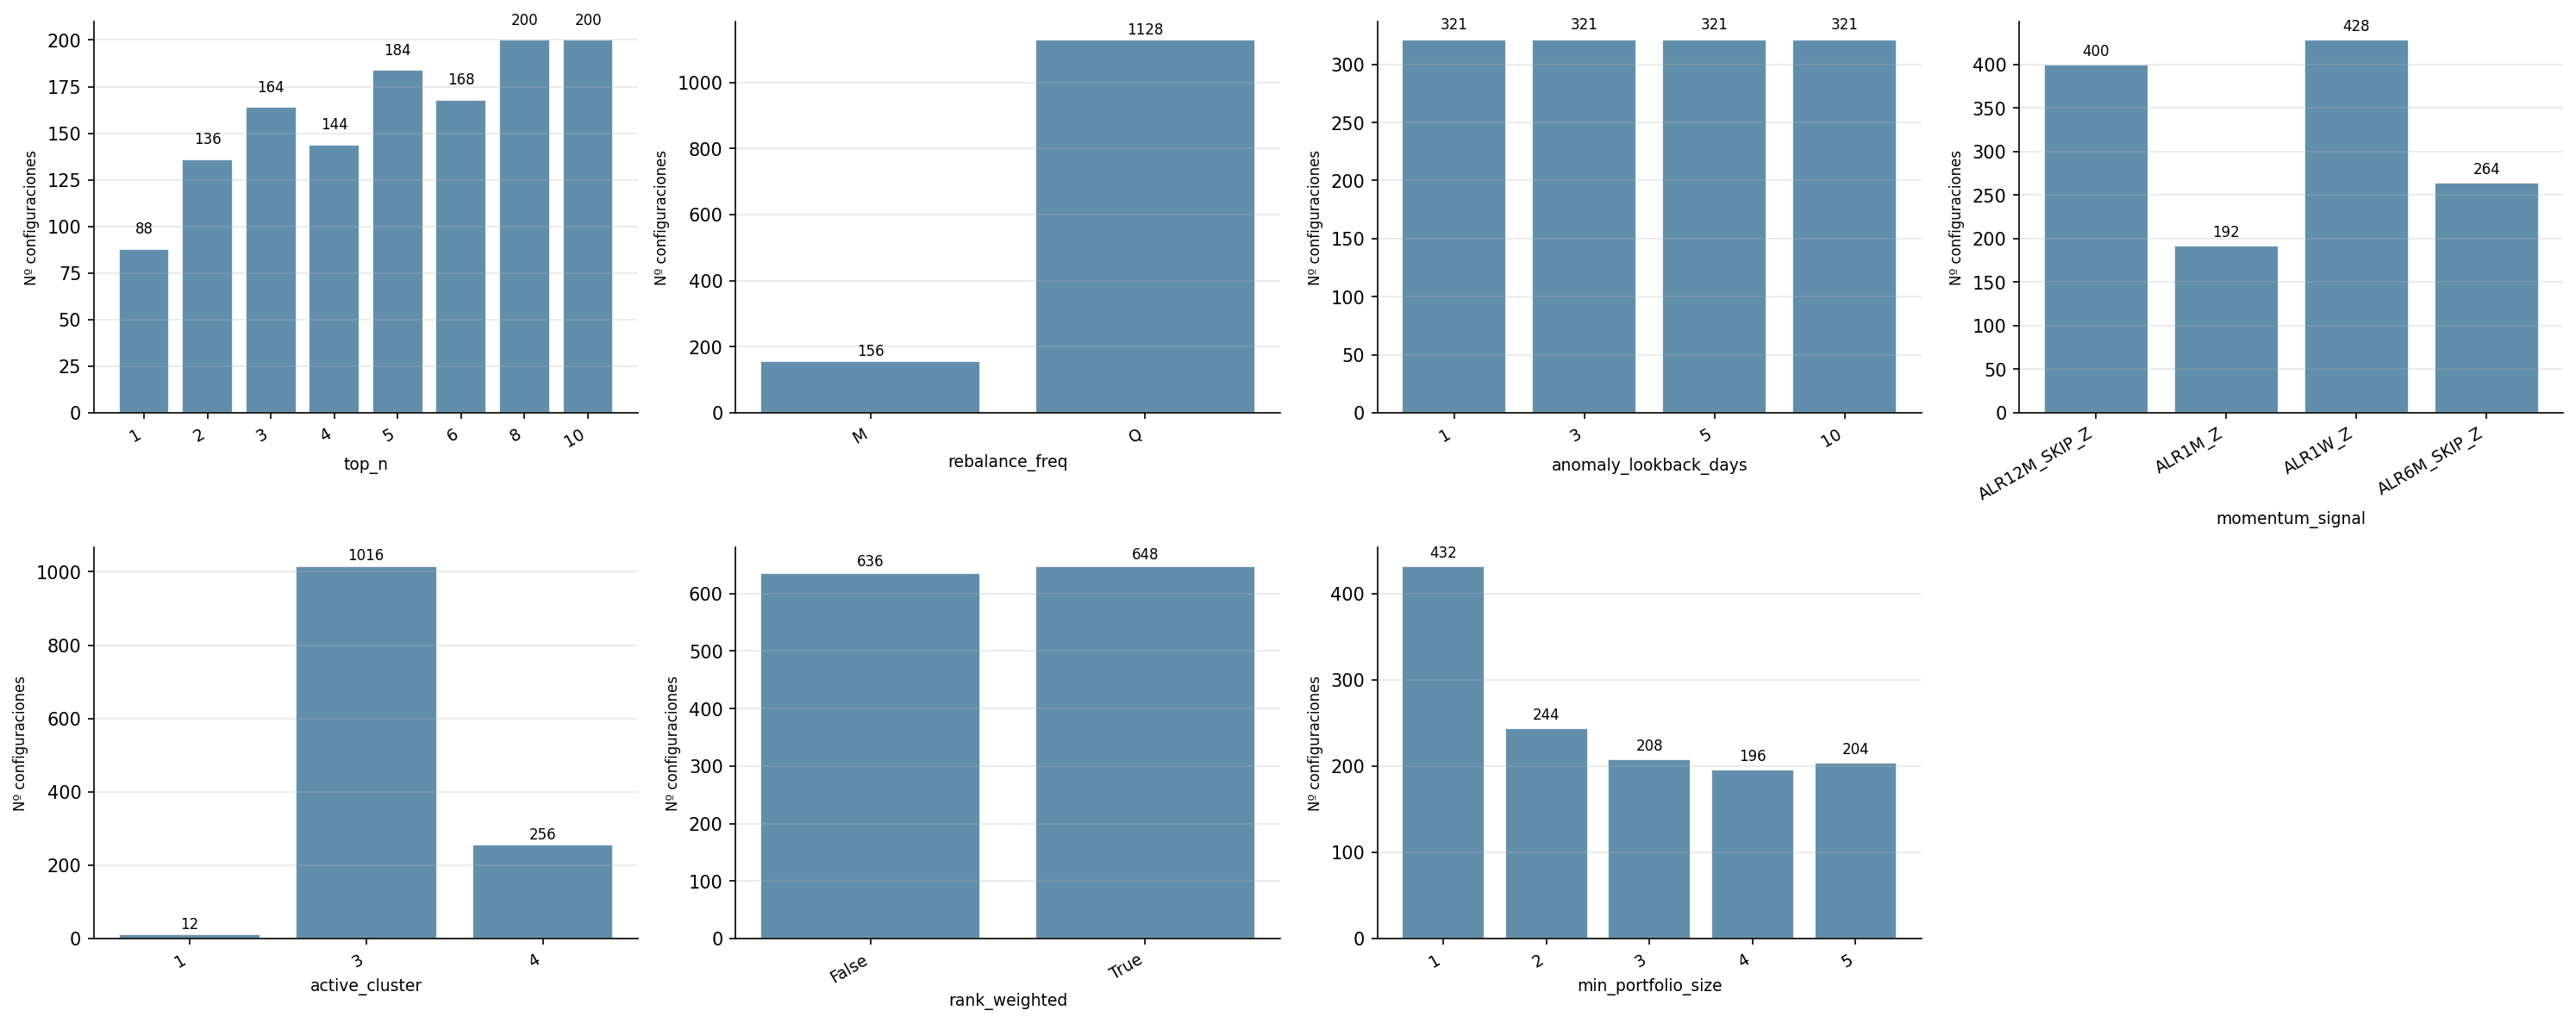
\includegraphics[width=\textwidth]{media/wf_04_hyperparameter_distribution.png}
    \caption{Distribución de hiperparámetros en el Top 10\,\%
    del Grid Search In-Sample. Cada barra representa el número de
    configuraciones (las mejores) que utilizan un valor concreto del
    parámetro. Fuente: Elaboración propia.}
    \label{fig:hyperparam_dist}
\end{figure}

Se observa que el parámetro \texttt{active\_cluster} presenta una
frecuencia enormemente concentrada en el valor 3 (Pullback
alcista), lo que indica que este régimen de mercado ofrece las
condiciones más favorables para la generación de señales de
momentum. Por el contrario, los clústeres 0 (Bajista moderado)
y 4 (Estrés/Capitulación) aparecen de forma marginal,
confirmando la interpretación económica desarrollada en el
Capítulo 4.

El rebalanceo trimestral (\texttt{Q}) domina ampliamente sobre el
mensual, los tamaños de cartera más frecuentes son
\texttt{top\_n=10} y \texttt{top\_n=8}, seguidos de
\texttt{top\_n=5} y \texttt{top\_n=3}, y la ponderación por ranking
(\texttt{rank\_weighted=True}) aparece con una frecuencia
ligeramente superior a la equiponderada, aunque ambas están
prácticamente equilibradas.

\paragraph{Top 5 combinaciones en entrenamiento}

La Tabla~\ref{tab:top5_is} presenta las cinco configuraciones con
mejor ratio de Sharpe dentro de la muestra de entrenamiento.

\begin{table}[H]
\centering
\small
\begin{tabular}{clcccccc}
\toprule
\textbf{\#} & \textbf{Señal} & \textbf{Cl.} & \textbf{Freq.} & \textbf{Top} &
\textbf{RW} & \textbf{Sharpe} & \textbf{CAGR (\%)} \\
\midrule
1 & ALR1W\_Z  & 3 & Q & 3 & No  & \textbf{1,366} & 26,63 \\
2 & ALR1W\_Z  & 3 & Q & 4 & Sí  & 1,298         & 26,78 \\
3 & ALR1W\_Z  & 3 & Q & 3 & No  & 1,293         & 24,84 \\
4 & ALR1W\_Z  & 3 & Q & 3 & Sí  & 1,285         & 26,91 \\
5 & ALR1W\_Z  & 3 & Q & 4 & No  & 1,281         & 25,34 \\
\bottomrule
\end{tabular}
\caption{Top 5 configuraciones del Grid Search In-Sample.
Fuente: Elaboración propia.}
\label{tab:top5_is}
\begin{flushleft}
\small \textit{Nota:} \textbf{Cl.}=active\_cluster,
\textbf{Freq.}=rebalance\_freq, \textbf{RW}=rank\_weighted.
\end{flushleft}
\end{table}

Se observa que la configuración óptima en entrenamiento alcanza
un ratio de Sharpe de 1,366 con una rentabilidad anualizada del
\SI{26,63}{\percent} y una caída máxima de únicamente \SI{-7.22}{\percent}. La
señal \texttt{ALR1W\_Z}, el clúster 3, el rebalanceo trimestral
y un tamaño de cartera reducido (\texttt{top\_n=3}) son los
elementos comunes a todas las configuraciones del Top 5.

No obstante, estas métricas deben interpretarse con cautela, ya
que reflejan el rendimiento sobre los mismos datos utilizados
para seleccionar la configuración. Habría que comprobar, tal y como se hará posteriormente, si este
rendimiento se mantiene al aplicarse sobre datos no vistos.


\subsubsection{Validación en Test}

Para evaluar la capacidad de generalización del sistema, las
1.280 configuraciones del Top 10\,\% en Sharpe de entrenamiento
se re-evaluaron sobre la ventana de prueba, que comprende el
último año de datos de mercado. 

\paragraph{Degradación del rendimiento}

La Tabla~\ref{tab:degradacion} muestra el comportamiento del conjunto de configuraciones al pasar de la ventana
de entrenamiento a la ventana de prueba.

\begin{table}[H]
\centering
\begin{tabular}{lrr}
\toprule
\textbf{Métrica} & \textbf{Train} & \textbf{Test} \\
\midrule
Sharpe medio                & 0,996   & 0,176    \\
CAGR medio (\%)             & 21,47   & 4,12     \\
Caída máxima media (\%)     & -17,82  & -18,24   \\
Proporción Sharpe $>$ 0 (\%)& 100,0   & 55,9     \\
Degradación de Sharpe media & ---     & 0,821    \\
\bottomrule
\end{tabular}
\caption{Métricas del proceso de validación sobre
1.280 configuraciones. Fuente: Elaboración propia.}
\label{tab:degradacion}
\end{table}

El descenso del Sharpe medio desde 0,996 hasta 0,176, con una
degradación media de 0,821 puntos, muestra la presencia de
sobreajuste (\textit{overfitting}) en el proceso
de selección. Esto es esperable y constituye una
característica común a cualquier proceso de optimización de
hiperparámetros sobre datos históricos.

Sin embargo, es relevante destacar que más de la mitad de las
configuraciones (55,9\,\%) mantienen un ratio de Sharpe positivo
en la ventana de prueba, lo que indica que existe un subconjunto de
estrategias con capacidad real de generalización.

\paragraph{La paradoja del campeón aparente}

La Figura~\ref{fig:sharpe_scatter} presenta un diagrama de
dispersión que muestra el Sharpe en entrenamiento (eje X)
frente al Sharpe en prueba (eje Y) para cada una de las 1.280
configuraciones evaluadas. Los puntos situados sobre la diagonal
representan estrategias que son consistentes; los que se
sitúan por debajo muestran degradación.

\begin{figure}[H]
    \centering
    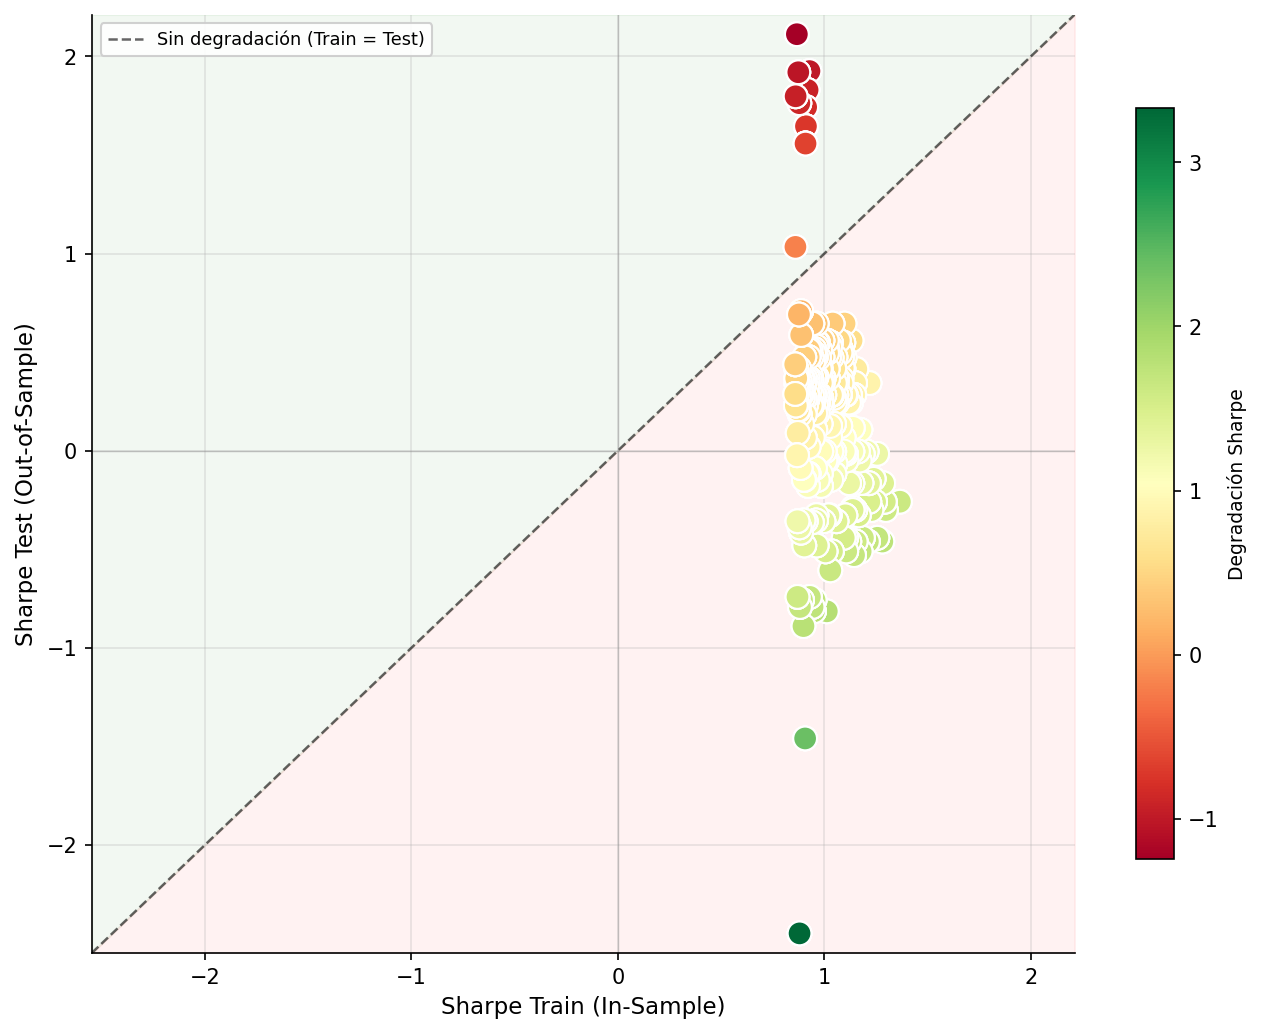
\includegraphics[width=0.8\textwidth]{media/wf_03_sharpe_scatter.png}
    \caption{Dispersión Sharpe Train vs.\ Sharpe Test. Cada punto
    representa una configuración. El color codifica la magnitud
    de la degradación (verde: baja, rojo: alta).
    Fuente: Elaboración propia.}
    \label{fig:sharpe_scatter}
\end{figure}

Se observa un fenómeno relevante: la configuración
con mejor Sharpe en entrenamiento (1,366) se sitúa en la zona
inferior del gráfico, con un Sharpe en prueba de \(-0,259\). Es
decir, la mejor estrategia aparente es, precisamente, la que más
fracasa al enfrentarse a datos nuevos. Este resultado constituye
una demostración de sobreajuste y muestra la
necesidad de la validación con datos no vistos.

Por el contrario, las configuraciones que mejores resultados
obtienen en Test no son las que lideraban el ranking en
entrenamiento. Esto refleja la existencia de
estrategias que, sin alcanzar los valores extremos de Sharpe en
la muestra de entrenamiento, poseen una estructura menos
sensible al ruido del periodo histórico.

\paragraph{Análisis de la degradación por ranking}

La Figura~\ref{fig:degradation_bar} muestra las barras
comparativas del ratio de Sharpe en entrenamiento y en prueba
para las configuraciones extremas del ranking. Se han
seleccionado las 15 configuraciones con menor Sharpe de
entrenamiento y las 15 con mayor Sharpe de entrenamiento.

\begin{figure}[H]
    \centering
    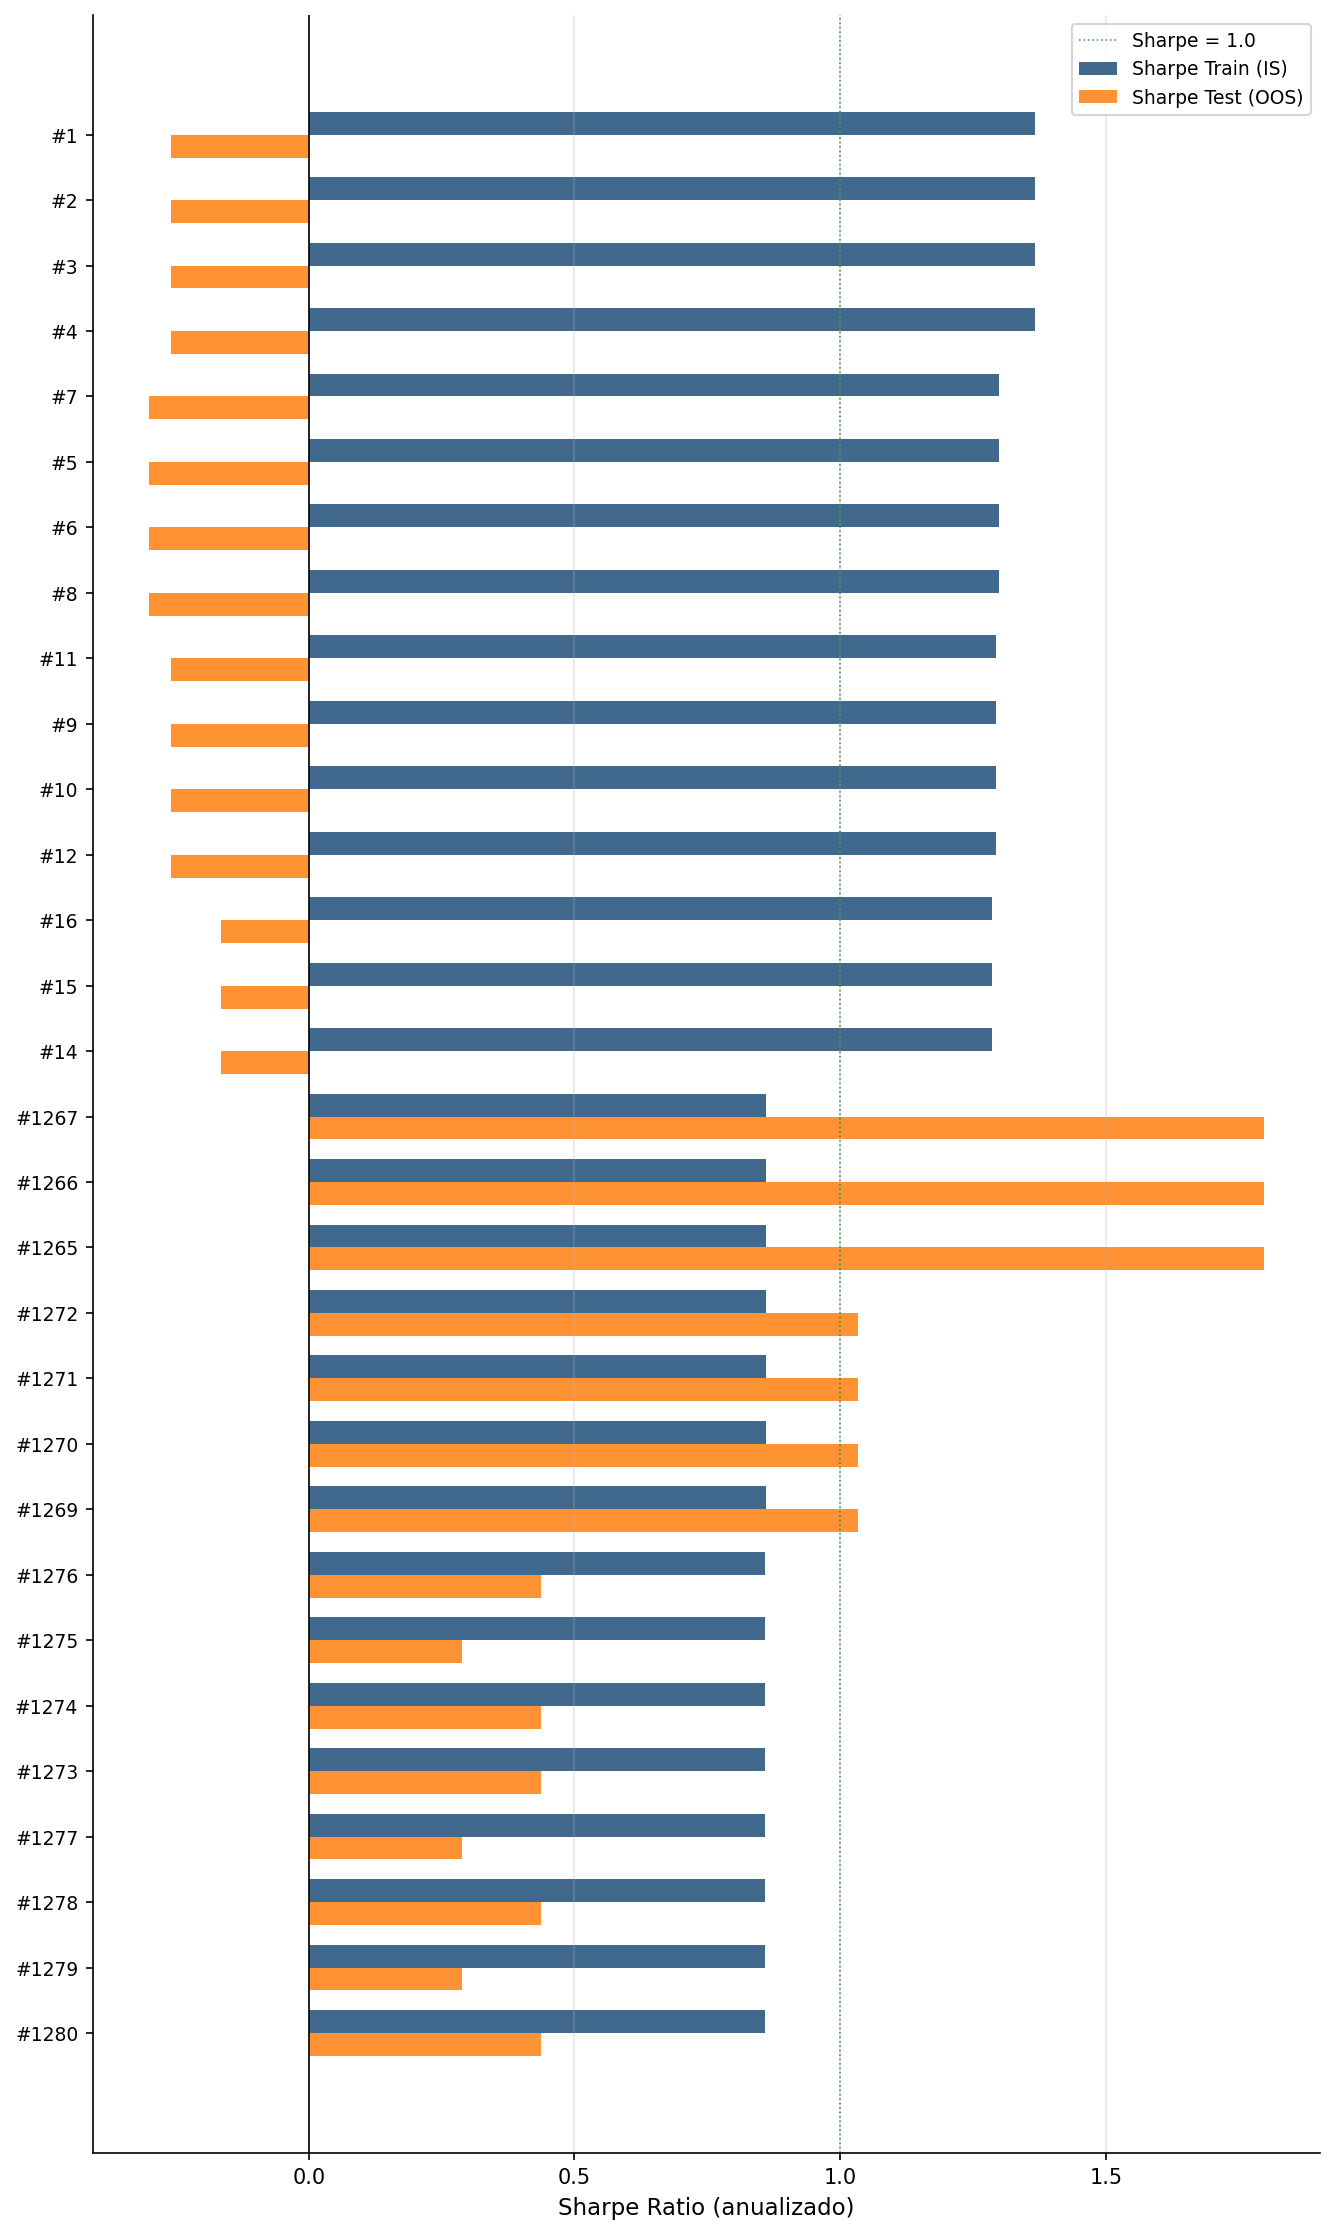
\includegraphics[width=0.85\textwidth]{media/wf_05_degradation_bar.png}
    \caption{Comparación del Sharpe en Train (azul) y en
    Test (naranja) para las configuraciones extremas. Se observa
    que las configuraciones con mayor Sharpe en entrenamiento
    presentan una degradación más elevada. Fuente: Elaboración propia.}
    \label{fig:degradation_bar}
\end{figure}

Se observa que las configuraciones con Sharpe de
entrenamiento más elevados muestran una caída
mayor en la ventana de Test. Este comportamiento refuerza la
necesidad de no confiar exclusivamente en las métricas de
entrenamiento para la selección del modelo final.

Por el contrario, las configuraciones con Sharpe de entrenamiento
moderado (en torno a 0,8--1,0) presentan, en muchos casos, una
degradación menor o incluso nula, lo que sugiere que estas
estrategias poseen una estructura más robusta.

\paragraph{Identificación de la mejor configuración global}

Se identifican las
configuraciones con mejor rendimiento en la ventana de prueba.
La Tabla~\ref{tab:top10_oos} presenta las diez estrategias con
Sharpe más elevado en datos no vistos.

\begin{table}[H]
\centering
\small
\begin{tabular}{clccccrr}
\toprule
\textbf{\#} & \textbf{Señal} & \textbf{Cl.} & \textbf{Freq.} & \textbf{Top} &
\textbf{RW} & \textbf{Sharpe\_Test} & \textbf{CAGR (\%)} \\
\midrule
1  & ALR1M\_Z    & 1 & M  & 8  & No  & \textbf{2,113} & 28,47 \\
2  & ALR1W\_Z    & 4 & M  & 3  & Sí  & 1,926         & 13,63 \\
3  & ALR1W\_Z    & 1 & M  & 10 & No  & 1,920         & 22,14 \\
4  & ALR1W\_Z    & 4 & M  & 4  & Sí  & 1,830         & 16,74 \\
5  & ALR1W\_Z    & 4 & M  & 5  & Sí  & 1,798         & 17,95 \\
6  & ALR1W\_Z    & 1 & M  & 10 & Sí  & 1,763         & 22,13 \\
7  & ALR1W\_Z    & 4 & M  & 2  & Sí  & 1,743         & 6,32  \\
8  & ALR1W\_Z    & 3 & Q  & 1  & No  & 1,646         & 16,72 \\
9  & ALR1W\_Z    & 3 & Q  & 1  & Sí  & 1,646         & 16,72 \\
10 & ALR1W\_Z    & 4 & M  & 3  & No  & 1,559         & 19,01 \\
\bottomrule
\end{tabular}
\caption{Top 10 configuraciones por Sharpe en Test.
Fuente: Elaboración propia.}
\label{tab:top10_oos}
\begin{flushleft}
\small \textit{Nota:} \textbf{Cl.}=active\_cluster,
\textbf{Freq.}=rebalance\_freq, \textbf{RW}=rank\_weighted.
\end{flushleft}
\end{table}

La mejor configuración global alcanza un ratio de Sharpe en
Test de 2,113, correspondiente a la señal \texttt{ALR1M\_Z}
(momento a un mes) sobre el clúster 1 (Bear market rally) con
rebalanceo mensual y tamaño de cartera \texttt{top\_n=8}. No
obstante, debe señalarse que este valor excepcional puede estar
influido por las condiciones específicas del periodo de prueba.

Las nueve configuraciones restantes del Top 10 comparten la
señal \texttt{ALR1W\_Z} (momento a una semana), lo que indica
que las señales de corto plazo son las que mejor se adaptan a
las condiciones del periodo de prueba. Destaca la diversidad
de regímenes representados: el clúster 4 (Estrés/Capitulación)
aparece en cinco configuraciones, el clúster 1 (Bear market
rally) en tres y el clúster 3 (Pullback alcista) en dos. El
rebalanceo mensual es mayoritario (ocho de diez), mientras que
la ponderación por ranking y la equiponderada se reparten al
50\,\%.

La configuración que ofrece el mejor equilibrio entre Sharpe
y rentabilidad dentro del grupo \texttt{ALR1W\_Z} es la que
combina el clúster 1 con \texttt{top\_n=10} y ponderación
equiponderada, alcanzando un Sharpe en Test de 1,920 y una
CAGR del 22,14\,\%.

\paragraph{Curva de capital de la configuración ganadora}

La Figura~\ref{fig:equity_winner} muestra la evolución del
capital acumulado de la mejor configuración en Test,
expresada en términos de mark-to-market diario real, frente al
índice de referencia SPY. La línea vertical punteada marca la
separación entre la ventana de entrenamiento y la ventana de
prueba.

\begin{figure}[H]
    \centering
    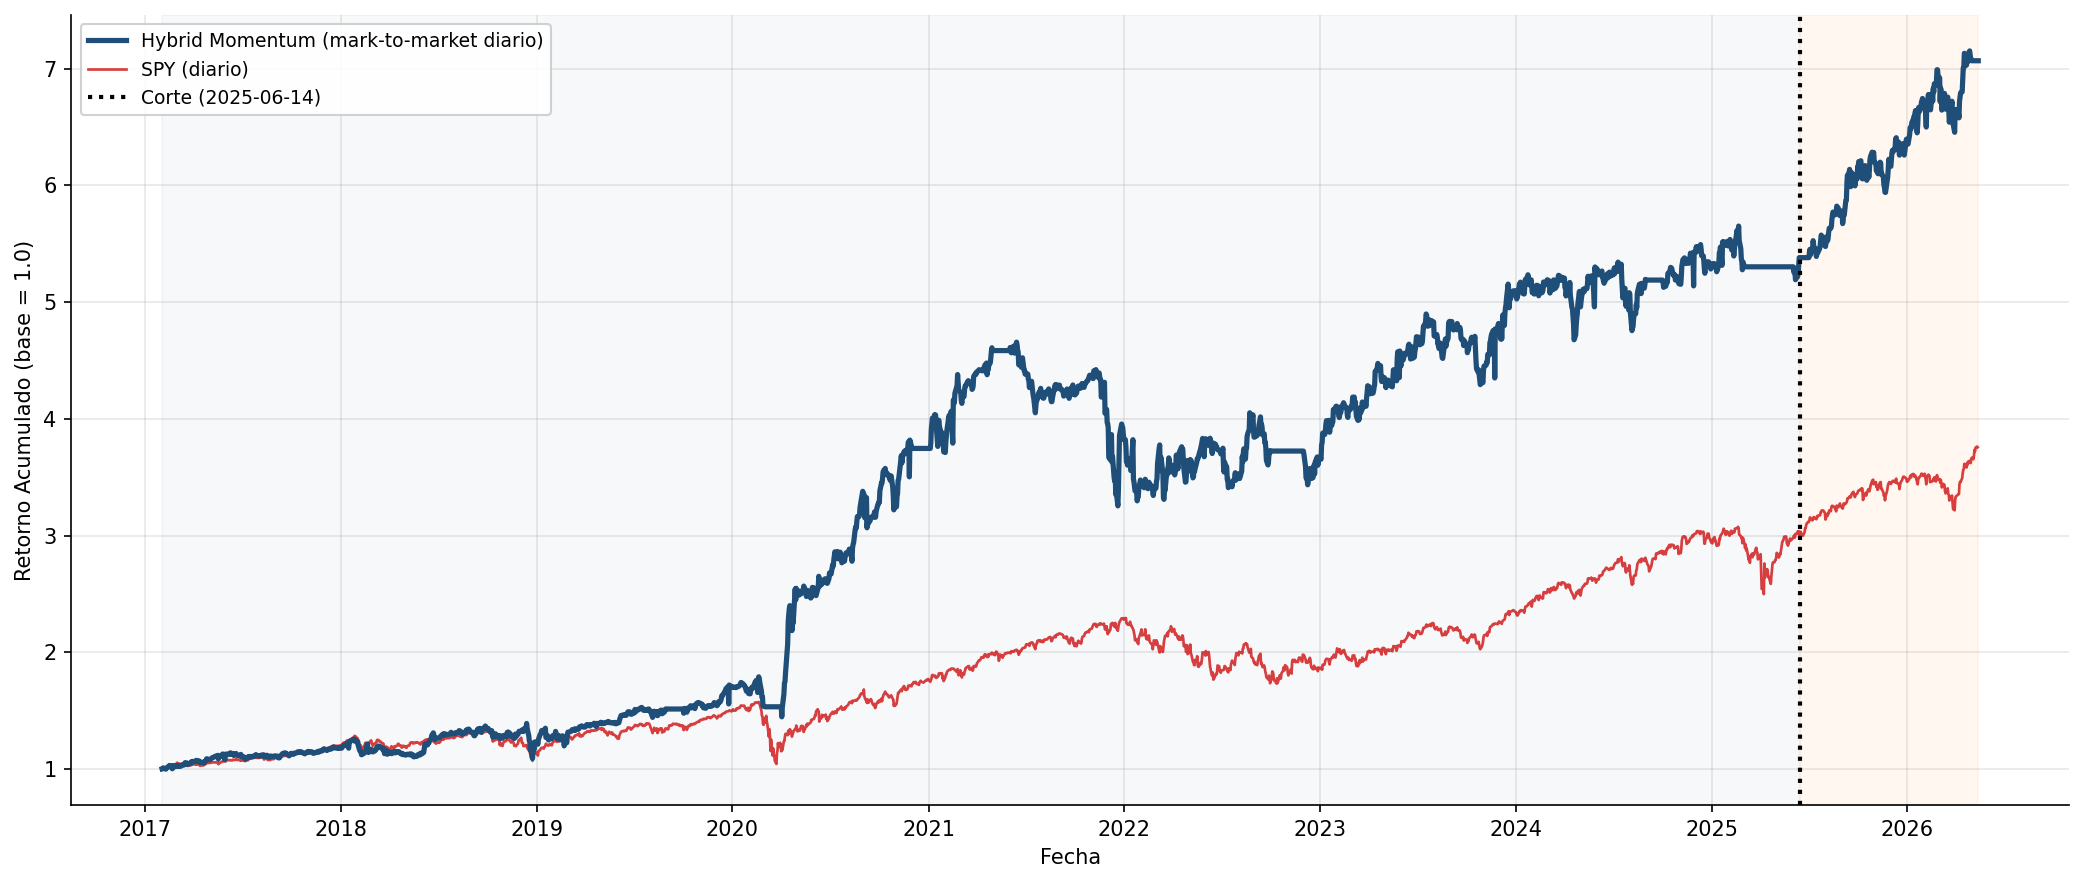
\includegraphics[width=\textwidth]{media/wf_01_equity_curve_winner_daily.png}
    \caption{Curva de capital de la mejor configuración
    en Test con resolución diaria frente al benchmark SPY.
    La línea vertical indica el inicio de la ventana de prueba.
    Fuente: Elaboración propia.}
    \label{fig:equity_winner}
\end{figure}

Se aprecia que la estrategia mantiene una trayectoria
ascendente consistente durante todo el periodo analizado,
acumulando una rentabilidad superior a la del
índice de referencia. La pendiente sostenida de la curva,
especialmente durante la ventana de prueba, sugiere que el
sistema es capaz de extraer señales de valor añadido de forma
consistente.

\paragraph{Comparativa con el índice de referencia SPY}

La Tabla~\ref{tab:comparativa_spy} presenta una comparación
entre las métricas de la mejor configuración
en Test y las del índice de referencia SPY.

\begin{table}[H]
\centering
\begin{tabular}{lrrr}
\toprule
\textbf{Métrica} & \textbf{Estrategia} & \textbf{SPY} \\
\midrule
Sharpe                & 2,113 & 0,585 \\
CAGR (\%)             & 28,47 & 12,10 \\
Caída máxima (\%)     & -4,05 & -12,10 \\
\bottomrule
\end{tabular}
\caption{Comparativa de la mejor configuración en Test frente al
benchmark SPY. Fuente: Elaboración propia.}
\label{tab:comparativa_spy}
\end{table}

La estrategia triplica prácticamente el ratio de Sharpe
del índice de referencia (2,113 frente a 0,585) y más que duplica
la rentabilidad anualizada (28,47\,\% frente a 12,10\,\%),
con una caída máxima notablemente inferior (-4,05\,\% frente a
-12,10\,\%). El sistema propuesto es capaz de generar
\textit{alpha} sobre el mercado de referencia.


\paragraph{Selección del modelo final}

Del análisis anterior se identifica como configuración de
referencia la estrategia \textbf{ALR1M\_Z} sobre el clúster 1
(Bear market rally), con rebalanceo mensual,
\texttt{top\_n=8} y ponderación equiponderada.

El criterio que justifica esta selección es:

\begin{itemize}
    \item \textbf{Rendimiento superior.} La estrategia triplica el
    Sharpe del índice de referencia (2,113 frente a 0,585) y más
    que duplica la rentabilidad anualizada (28,47\,\% frente a
    12,10\,\%), con una caída máxima de solo -4,05\,\% frente al
    -12,10\,\% del SPY.

    
\end{itemize}

No obstante, debe señalarse que este resultado excepcional
podría estar influido por las condiciones específicas del
periodo de prueba. Como alternativa más conservadora, las
configuraciones basadas en \texttt{ALR1W\_Z} ofrecen un
respaldo estadístico más amplio al concentrar nueve de las
diez posiciones del Top 10.

Los parámetros completos se resumen en la
Tabla~\ref{tab:modelo_final}.

\begin{table}[H]
\centering
\small
\begin{tabular}{ll}
\toprule
\textbf{Parámetro} & \textbf{Valor} \\
\midrule
Señal de momentum    & ALR1M\_Z (1 mes) \\
Clúster              & 1 (Bear market rally) \\
Rebalanceo           & Mensual (M) \\
Tamaño de cartera    & \texttt{top\_n=8} (8 activos) \\
Ponderación          & Equiponderada \\
Ventana anomalías    & 1 día \\
Tamaño mínimo cartera& 1 (sin mínimo exigido) \\
\bottomrule
\end{tabular}
\caption{Parámetros del modelo final seleccionado.
Fuente: Elaboración propia.}
\label{tab:modelo_final}
\end{table}


\subsubsection{Análisis de Robustez}

Esta sección aborda la cuestión de si los resultados obtenidos
pueden considerarse estadísticamente fiables o si, por el
contrario, responden a patrones 'falsos' propios del periodo de
evaluación.

\paragraph{Importancia de los hiperparámetros}

Para determinar qué parámetros del sistema ejercen una influencia
determinante sobre el rendimiento fuera de muestra, se ha
entrenado un modelo de bosque aleatorio (\textit{Random Forest})
con 300 árboles para predecir el Sharpe en prueba a partir de los
hiperparámetros de cada configuración. La
Tabla~\ref{tab:feature_importance} presenta la importancia
relativa de cada variable en la predicción.

\begin{table}[H]
\centering
\begin{tabular}{lr}
\toprule
\textbf{Variable} & \textbf{Importancia (\%)} \\
\midrule
top\_n                   & 25,99 \\
min\_portfolio\_size     & 23,64 \\
active\_cluster          & 21,01 \\
momentum\_signal         & 20,12 \\
rebalance\_freq          & 6,02  \\
rank\_weighted           & 3,22  \\
anomaly\_lookback\_days  & 0,01  \\
\bottomrule
\end{tabular}
\caption{Importancia de los hiperparámetros en la predicción del
Sharpe en Test mediante Random Forest. Fuente: Elaboración propia.}
\label{tab:feature_importance}
\end{table}

Los resultados revelan que los tres parámetros con mayor impacto
son \texttt{top\_n} (tamaño de la cartera), \texttt{min\_portfolio\_size}
(tamaño mínimo para evitar periodos en efectivo) y
\texttt{active\_cluster} (régimen de mercado seleccionado), que
conjuntamente explican más del 70\,\% de la varianza del
rendimiento fuera de muestra. La señal de momentum contribuye
con un 20\,\% adicional.

Resulta especialmente relevante la contribución prácticamente
nula del parámetro \texttt{anomaly\_lookback\_days} (ventana de
retrospectiva para el filtro DBSCAN). Este hallazgo sugiere que
la presencia del filtro topológico es importante para la
integridad del sistema, pero la longitud de la ventana de
observación de anomalías no es un factor determinante del
rendimiento, probablemente porque el filtro diario \textit{cross-
sectional} de DBSCAN proporciona una protección suficientemente
robusta con independencia del horizonte retrospectivo concreto
utilizado.

\paragraph{Sensibilidad de parámetros en ventana de prueba}

La Figura~\ref{fig:oos_sensitivity} descompone el rendimiento en Test agregado de las 1.064 configuraciones con Sharpe
de prueba válido, agrupándolas por el valor de cada
hiperparámetro. Para cada parámetro, se reconstruye la curva de
capital diaria de todas las configuraciones que comparten ese
valor y se promedia, permitiendo aislar visualmente el efecto
marginal de cada variable sobre el rendimiento conjunto.

\begin{figure}[H]
    \centering
    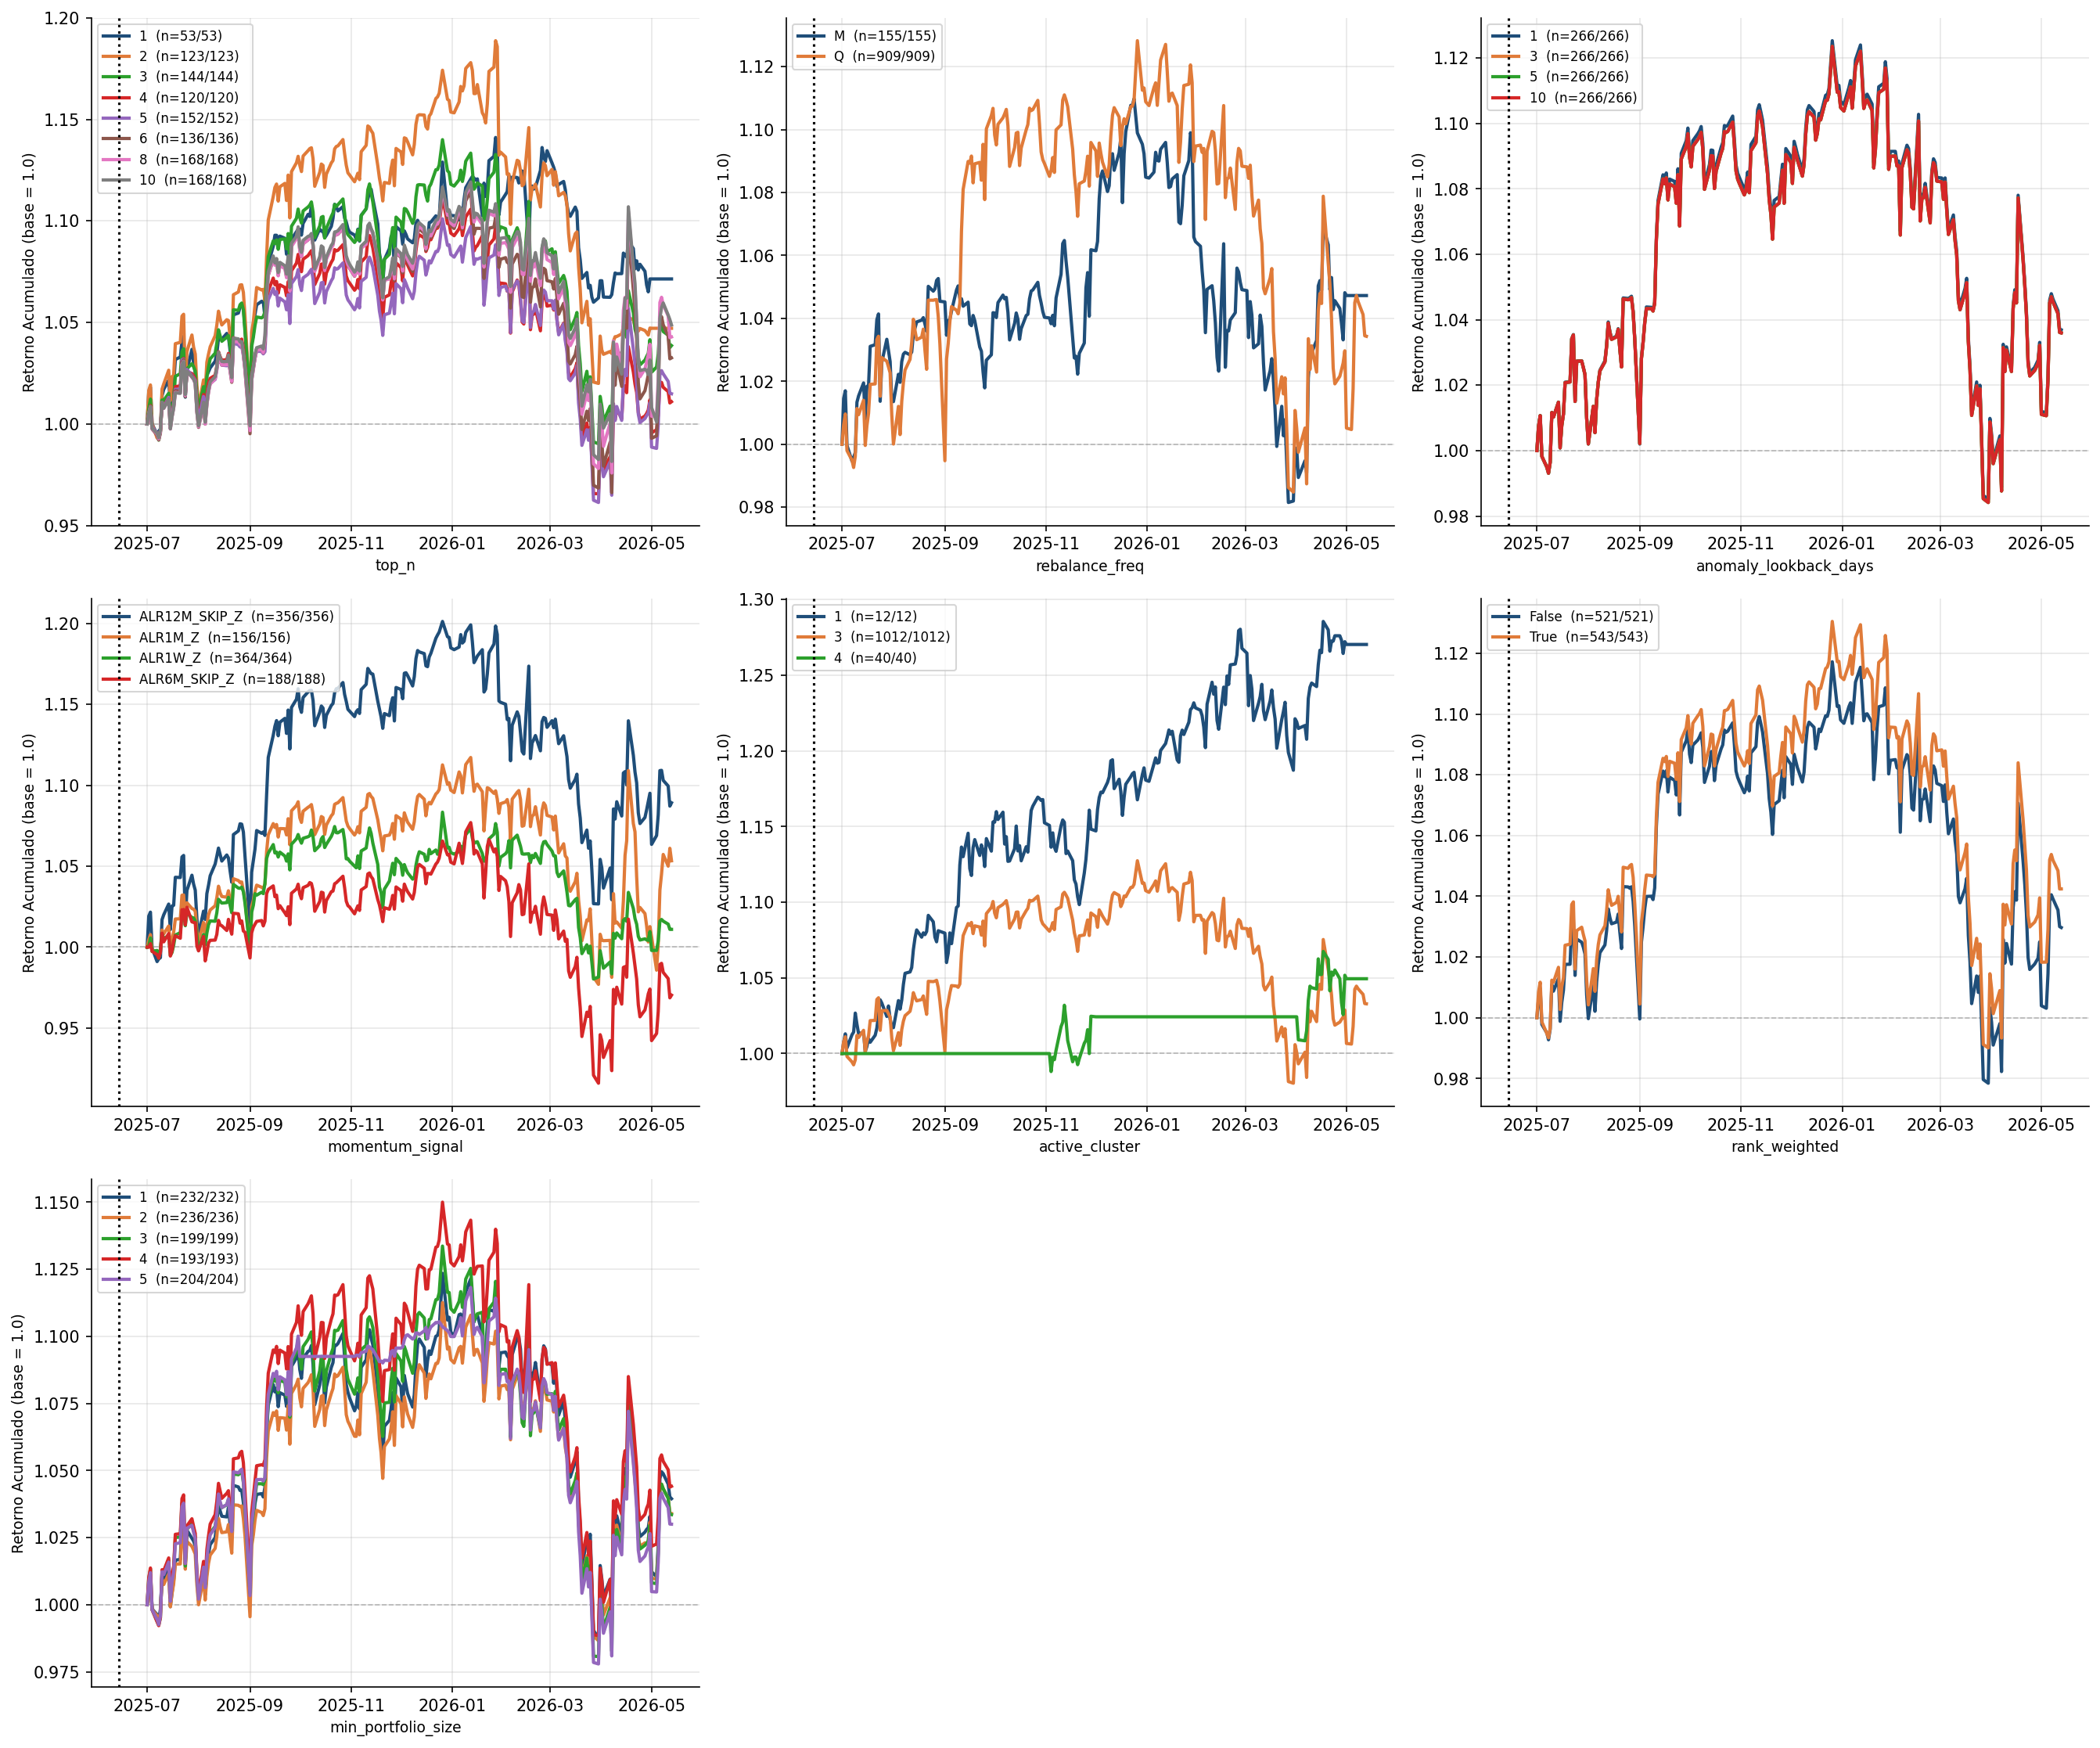
\includegraphics[width=1.05\textwidth]{media/wf_07_oos_parameter_sensitivity.png}
    \caption{Curvas de capital medias Out-of-Sample agrupadas por
    valor de hiperparámetro. Cada panel desagrega el efecto de
    una variable sobre el rendimiento agregado del conjunto de
    configuraciones (\textit{N}=1.064). Fuente: Elaboración propia.}
    \label{fig:oos_sensitivity}
\end{figure}

Se observa que:
\begin{itemize}
    
    \item \textbf{active\_cluster}: el clúster 1 es el que
    presenta el rendimiento acumulado medio más elevado (final
    de 1,270), seguido del clúster 4 (1,050). El clúster 3,
    pese a concentrar el 95\,\% de las configuraciones,
    muestra la curva media más baja (1,033).
    
    \item \textbf{rebalance\_freq}: la frecuencia mensual
    (\texttt{M}) supera a la trimestral en rendimiento acumulado
    medio (1,047 frente a 1,034), pese a que esta última
    concentra el 85\,\% de las configuraciones.
    \item \textbf{rank\_weighted}: la ponderación por ranking
    ofrece un rendimiento ligeramente superior a la
    equiponderada (1,042 frente a 1,030), aunque la diferencia
    es muy leve y ambas opciones generan rentabilidad positiva
    en promedio.
\end{itemize}

\paragraph{Conclusiones del capítulo}

Los resultados presentados a lo largo de este capítulo permiten
extraer las siguientes conclusiones consolidadas:

\begin{enumerate}
    \item \textbf{El sobreajuste existe y es significativo.} La
    mejor configuración en entrenamiento (Sharpe 1,366) presenta
    un rendimiento negativo en la ventana de prueba (\(-0,259\)).
    Este fenómeno es común a cualquier proceso de optimización
    sobre datos históricos y debe ser gestionado mediante
    validación con datos no vistos.

    \item \textbf{La robustez existe y es identificable.} El
    55,9\,\% de las configuraciones mantienen un Sharpe positivo
    en prueba, y la mejor de ellas alcanza un valor de 2,113
    (señal \texttt{ALR1M\_Z} sobre clúster 1, rebalanceo mensual,
    \texttt{top\_n=8}). Esta configuración se consolida como el
    modelo de referencia del sistema.

    \item \textbf{El sistema supera al benchmark de referencia.}
    Tanto en términos de Sharpe (2,113 frente a 0,585) como de
    CAGR (28,47\,\% frente a 12,10\,\%), la mejor configuración
    en Test triplica el rendimiento ajustado al riesgo del
    índice SPY, con una caída máxima notablemente inferior.

    \item \textbf{La selección del régimen de mercado es
    crítica.} El parámetro \texttt{active\_cluster} explica el
    21\,\% de la varianza del rendimiento fuera de muestra. El
    clúster 3 (Pullback alcista) se consolida como el régimen
    más favorable para estrategias basadas en momentum.

    \item \textbf{El filtro topológico DBSCAN es un componente
    estructural, no una variable de ajuste.} La ventana de
    retrospectiva para la detección de anomalías (\texttt{anomaly\_lookback\_days})
    presenta una importancia prácticamente nula en el modelo de
    predicción, lo que sugiere que la presencia del filtro DBSCAN proporciona una protección
    suficiente contra el ruido.
\end{enumerate}

A la vista de estos resultados, el modelo seleccionado como
configuración de referencia es la estrategia
\texttt{ALR1M\_Z} sobre el clúster 1, con rebalanceo
mensual, \texttt{top\_n=8} y ponderación equiponderada.
Esta configuración ofrece la mayor rentabilidad, superando
al índice de referencia SPY tanto en términos
de Sharpe como de rentabilidad anualizada.


\endinput

% =============================================================================

\subsection{Evaluación y Backtesting}

En este capítulo se describe la evaluación
diseñada para validar el modelo propuesto, se presentan
los resultados obtenidos tanto en la fase de
entrenamiento (Train) como en la fase de prueba
(Test) y se analiza la robustez de las
configuraciones analizadas. El objetivo fundamental es
determinar si la arquitectura DBSCAN + K-Means,
combinada con una selección dinámica por momentum, es capaz de
generar rentabilidades (teniendo en cuenta el riesgo) superiores a las de
un índice de referencia.

A lo largo del capítulo se analiza si existe una combinación de hiperparámetros que responda de forma estable a datos no vistos, se cuantifica la magnitud de la degradación por sobreajuste al seleccionar las mejores configuraciones en la muestra de entrenamiento, y se identifican los parámetros que tienen una influencia sobre el rendimiento en test.


\subsubsection{Sistema de Evaluación}

La validación del sistema se ha diseñado con el objetivo de
aproximar, en la medida de lo posible, un entorno real de
inversión. Para ello, se establecen una serie de criterios orientados a evitar sesgos y a garantizar que la
comparación entre estrategias sea homogénea.

\paragraph{Causalidad temporal ($T/T+1$)}

Las decisiones de inversión se generan únicamente con la
información disponible al cierre del último día hábil del período
de rebalanceo $T$. La entrada efectiva en cartera se realiza al
cierre del primer día hábil posterior ($T+1$). De esta forma,
se evita incorporar información futura en el proceso de decisión.

Los retornos de cada cartera se calculan desde el cierre de
$T+1$ hasta el cierre del siguiente período de rebalanceo.
Además, todas las transformaciones estadísticas utilizadas por
el modelo se estiman
exclusivamente con datos históricos disponibles en cada fecha
según la Ecuación~\ref{eq:zscore_rolling}.

\paragraph{Ventanas temporales y división Train/Test}

El periodo completo de análisis comprende desde enero de 2017
hasta la fecha más reciente disponible. Para garantizar la
independencia entre la fase de optimización y la fase de
validación, se establece un punto de corte dinámico situado
exactamente un año antes del momento de ejecución del
experimento:

\begin{itemize}
    \item \textbf{Ventana de entrenamiento (Train):}
    desde enero de 2017 hasta un año antes de la fecha actual.
    Sobre esta ventana se ejecuta el \textit{grid search}.
    \item \textbf{Ventana de prueba (Test):}
    desde la fecha de corte hasta la actualidad. Sobre esta
    ventana se evalúan exclusivamente las configuraciones
    seleccionadas en la fase de entrenamiento, sin ningún tipo
    de realimentación hacia el modelo.
\end{itemize}

\paragraph{Benchmark de referencia}

Como índice de comparación se utiliza el ETF \textit{SPDR
S\&P 500 ETF Trust} (SPY), ampliamente empleado como referencia de la renta variable estadounidense. Su curva de
capital se normaliza a base 1,0 en la misma fecha inicial que la
estrategia.

\paragraph{Arquitectura del proceso experimental}

El diseño sigue dos etapas diferenciadas, ilustrado en la
Figura~\ref{fig:experimental_design}:

\begin{enumerate}
    \item \textbf{Búsqueda en malla (\textit{Grid Search})
    con datos de entrenamiento}: Se enumeran las 12.800
    combinaciones resultantes de los
    siete hiperparámetros definidos en el sistema
    (\texttt{top\_n}, \texttt{rebalance\_freq},
    \texttt{anomaly\_lookback\_days}, \texttt{momentum\_signal},
    \texttt{active\_cluster}, \texttt{rank\_weighted} y
    \texttt{min\_portfolio\_size}). Cada combinación se evalúa
    sobre la ventana de entrenamiento y se registran sus
    métricas.

    \item \textbf{Validación con datos de prueba}: Se
    selecciona el 10\,\% de las configuraciones con mejor
    \textit{ratio de Sharpe} en la fase anterior (1.280 estrategias). Cada una de ellas se re-evalúa sobre la
    ventana de Test, cronológicamente posterior y nunca vista
    durante la optimización. Se mide la degradación del Sharpe
    como diferencia entre el valor en entrenamiento y en prueba,
    siendo la métrica central de sobreajuste.
\end{enumerate}

\begin{figure}[H]
    \centering
    \begin{tikzpicture}[node distance=1.5cm, auto,
        block/.style={rectangle, draw, text width=7cm,
        text centered, rounded corners, minimum height=0.8cm,
        font=\small},
        arrow/.style={draw, -latex', thick}]

        \node [block, fill=green!10] (grid)
            {Grid Search \\
             7 parámetros $\times$ 12.800 combinaciones \\
             Ventana: 2017 -- ($t-1$ año)};
        \node [block, below of=grid, fill=yellow!15] (top)
            {Selección Top 10\,\% por Sharpe \\
             $\approx$ 1.280 configuraciones \\};
        \node [block, below of=top, fill=cyan!15] (wf)
            {Evaluación en datos de prueba \\
             Ventana: ($t-1$ año) -- ($t$) \\
             Sharpe\_Test, Degradación};
        \node [block, below of=wf, fill=orange!15] (analysis)
            {Análisis de Robustez \\
             Importancia de parámetros, \\
             Sensibilidad, Comparativa vs SPY};

        \path [arrow] (grid) -- (top);
        \path [arrow] (top) -- (wf);
        \path [arrow] (wf) -- (analysis);
    \end{tikzpicture}
    \caption{Arquitectura del proceso experimental. Fuente: Elaboración propia.}
    \label{fig:experimental_design}
\end{figure}


\subsubsection{Búsqueda en malla (Grid Search) en datos de entrenamiento}

Sobre la ventana de entrenamiento se ejecuta un barrido de las 12.800 combinaciones de hiperparámetros
ya mencionadas. Todas las combinaciones
generaron resultados válidos.

\paragraph{Distribución del ratio de Sharpe en entrenamiento}

La Figura~\ref{fig:hyperparam_dist} muestra la distribución de
los siete hiperparámetros dentro del subconjunto de estrategias
que pertenecen al 10\,\% superior en Sharpe dentro de la muestra
de entrenamiento. Este análisis permite identificar qué valores
de cada parámetro aparecen con mayor frecuencia entre las mejores
configuraciones.

\begin{figure}[H]
    \centering
    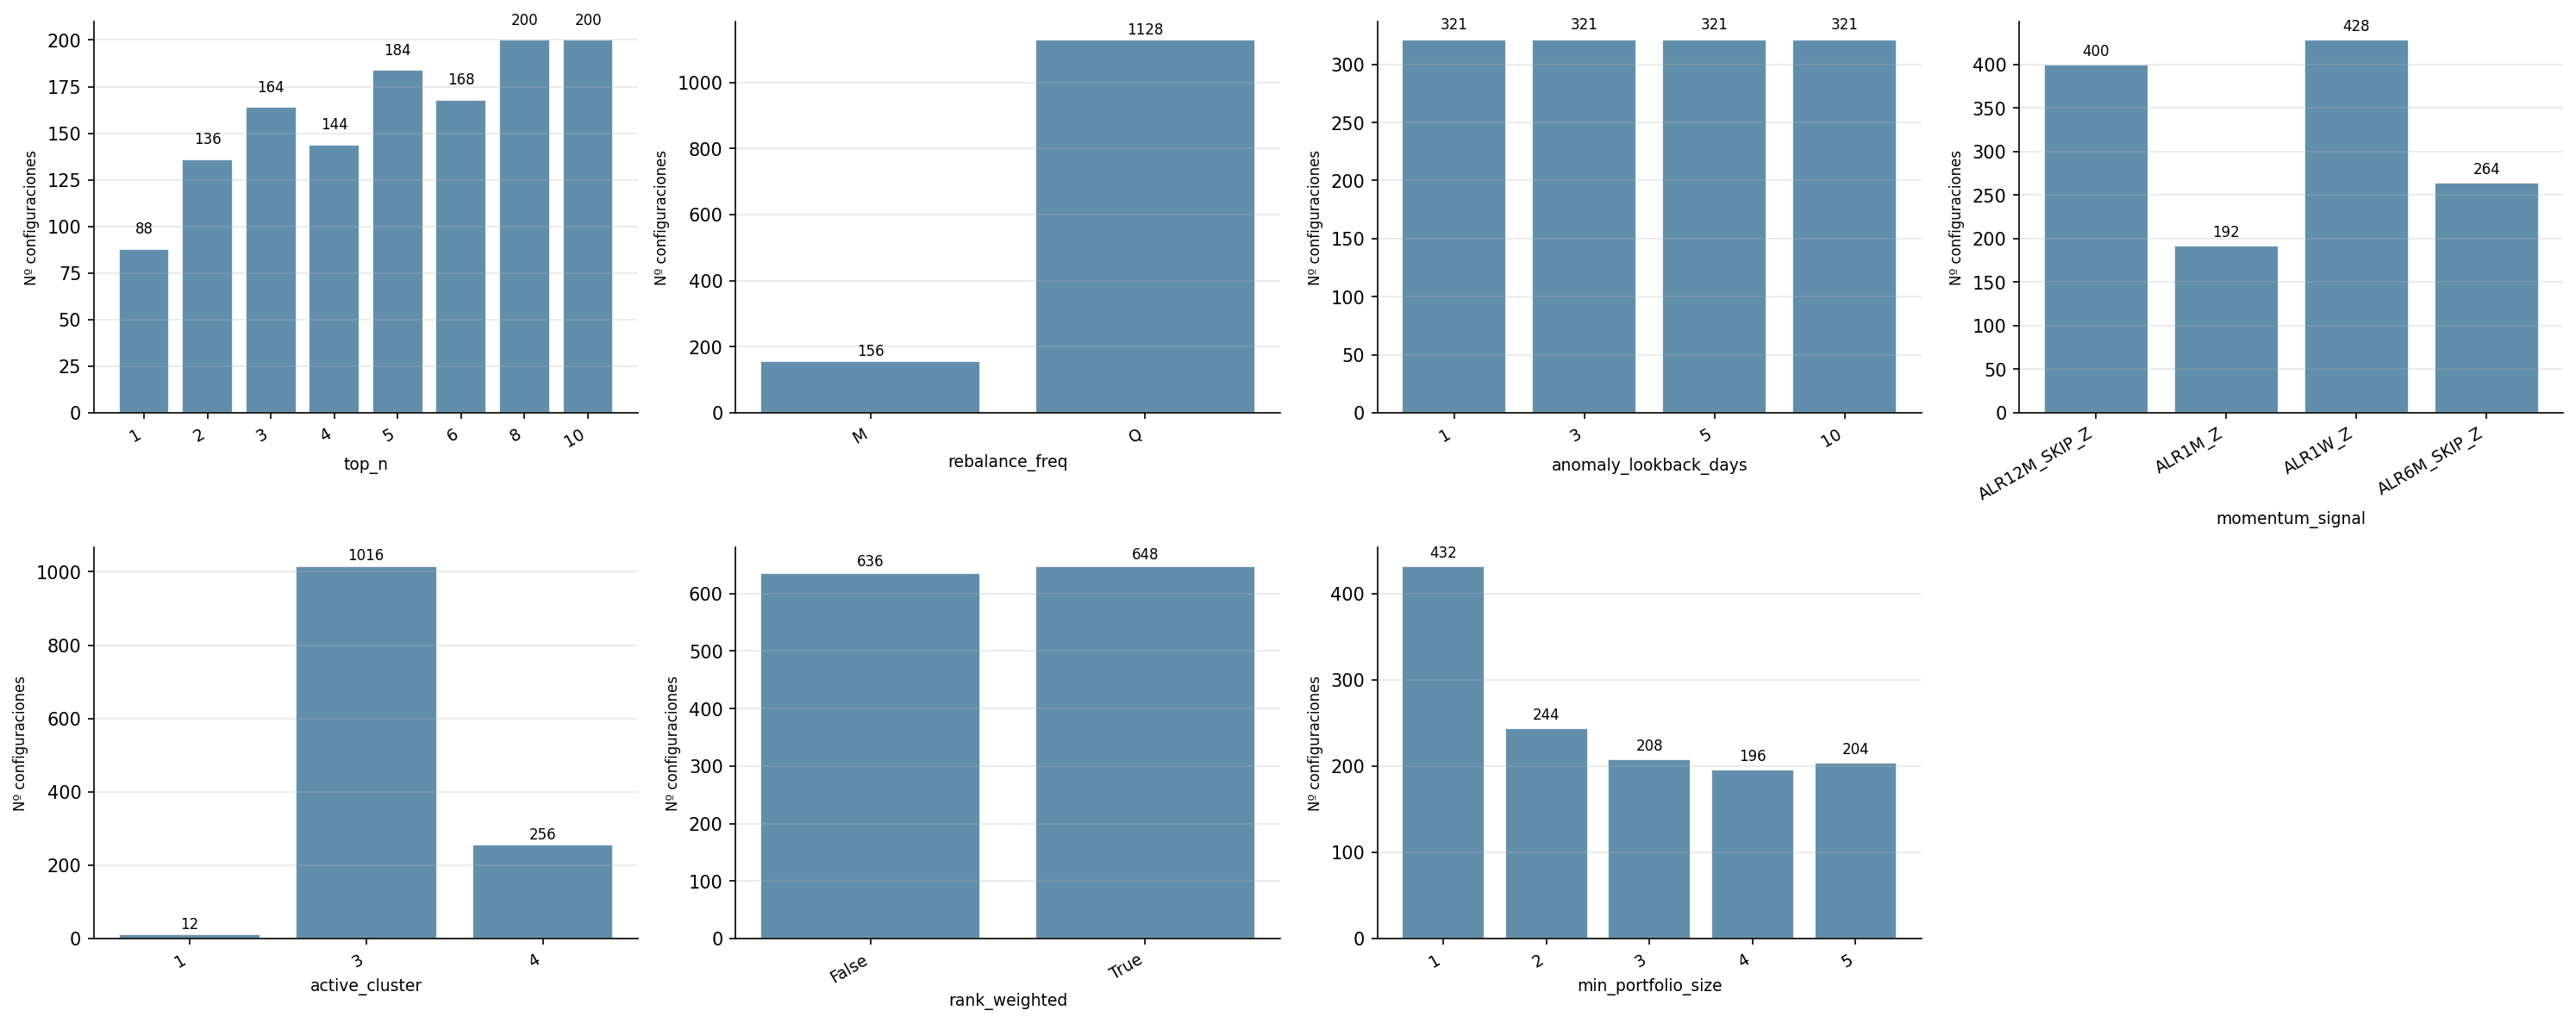
\includegraphics[width=\textwidth]{media/wf_04_hyperparameter_distribution.png}
    \caption{Distribución de hiperparámetros en el Top 10\,\%
    del Grid Search In-Sample. Cada barra representa el número de
    configuraciones (las mejores) que utilizan un valor concreto del
    parámetro. Fuente: Elaboración propia.}
    \label{fig:hyperparam_dist}
\end{figure}

Se observa que el parámetro \texttt{active\_cluster} presenta una
frecuencia enormemente concentrada en el valor 3 (Pullback
alcista), lo que indica que este régimen de mercado ofrece las
condiciones más favorables para la generación de señales de
momentum. Por el contrario, los clústeres 0 (Bajista moderado)
y 4 (Estrés/Capitulación) aparecen de forma marginal,
confirmando la interpretación económica desarrollada en el
Capítulo 4.

El rebalanceo trimestral (\texttt{Q}) domina ampliamente sobre el
mensual, los tamaños de cartera más frecuentes son
\texttt{top\_n=10} y \texttt{top\_n=8}, seguidos de
\texttt{top\_n=5} y \texttt{top\_n=3}, y la ponderación por ranking
(\texttt{rank\_weighted=True}) aparece con una frecuencia
ligeramente superior a la equiponderada, aunque ambas están
prácticamente equilibradas.

\paragraph{Top 5 combinaciones en entrenamiento}

La Tabla~\ref{tab:top5_is} presenta las cinco configuraciones con
mejor ratio de Sharpe dentro de la muestra de entrenamiento.

\begin{table}[H]
\centering
\small
\begin{tabular}{clcccccc}
\toprule
\textbf{\#} & \textbf{Señal} & \textbf{Cl.} & \textbf{Freq.} & \textbf{Top} &
\textbf{RW} & \textbf{Sharpe} & \textbf{CAGR (\%)} \\
\midrule
1 & ALR1W\_Z  & 3 & Q & 3 & No  & \textbf{1,366} & 26,63 \\
2 & ALR1W\_Z  & 3 & Q & 4 & Sí  & 1,298         & 26,78 \\
3 & ALR1W\_Z  & 3 & Q & 3 & No  & 1,293         & 24,84 \\
4 & ALR1W\_Z  & 3 & Q & 3 & Sí  & 1,285         & 26,91 \\
5 & ALR1W\_Z  & 3 & Q & 4 & No  & 1,281         & 25,34 \\
\bottomrule
\end{tabular}
\caption{Top 5 configuraciones del Grid Search In-Sample.
Fuente: Elaboración propia.}
\label{tab:top5_is}
\begin{flushleft}
\small \textit{Nota:} \textbf{Cl.}=active\_cluster,
\textbf{Freq.}=rebalance\_freq, \textbf{RW}=rank\_weighted.
\end{flushleft}
\end{table}

Se observa que la configuración óptima en entrenamiento alcanza
un ratio de Sharpe de 1,366 con una rentabilidad anualizada del
\SI{26,63}{\percent} y una caída máxima de únicamente \SI{-7.22}{\percent}. La
señal \texttt{ALR1W\_Z}, el clúster 3, el rebalanceo trimestral
y un tamaño de cartera reducido (\texttt{top\_n=3}) son los
elementos comunes a todas las configuraciones del Top 5.

No obstante, estas métricas deben interpretarse con cautela, ya
que reflejan el rendimiento sobre los mismos datos utilizados
para seleccionar la configuración. Habría que comprobar, tal y como se hará posteriormente, si este
rendimiento se mantiene al aplicarse sobre datos no vistos.


\subsubsection{Validación en Test}

Para evaluar la capacidad de generalización del sistema, las
1.280 configuraciones del Top 10\,\% en Sharpe de entrenamiento
se re-evaluaron sobre la ventana de prueba, que comprende el
último año de datos de mercado. 

\paragraph{Degradación del rendimiento}

La Tabla~\ref{tab:degradacion} muestra el comportamiento del conjunto de configuraciones al pasar de la ventana
de entrenamiento a la ventana de prueba.

\begin{table}[H]
\centering
\begin{tabular}{lrr}
\toprule
\textbf{Métrica} & \textbf{Train} & \textbf{Test} \\
\midrule
Sharpe medio                & 0,996   & 0,176    \\
CAGR medio (\%)             & 21,47   & 4,12     \\
Caída máxima media (\%)     & -17,82  & -18,24   \\
Proporción Sharpe $>$ 0 (\%)& 100,0   & 55,9     \\
Degradación de Sharpe media & ---     & 0,821    \\
\bottomrule
\end{tabular}
\caption{Métricas del proceso de validación sobre
1.280 configuraciones. Fuente: Elaboración propia.}
\label{tab:degradacion}
\end{table}

El descenso del Sharpe medio desde 0,996 hasta 0,176, con una
degradación media de 0,821 puntos, muestra la presencia de
sobreajuste (\textit{overfitting}) en el proceso
de selección. Esto es esperable y constituye una
característica común a cualquier proceso de optimización de
hiperparámetros sobre datos históricos.

Sin embargo, es relevante destacar que más de la mitad de las
configuraciones (55,9\,\%) mantienen un ratio de Sharpe positivo
en la ventana de prueba, lo que indica que existe un subconjunto de
estrategias con capacidad real de generalización.

\paragraph{La paradoja del campeón aparente}

La Figura~\ref{fig:sharpe_scatter} presenta un diagrama de
dispersión que muestra el Sharpe en entrenamiento (eje X)
frente al Sharpe en prueba (eje Y) para cada una de las 1.280
configuraciones evaluadas. Los puntos situados sobre la diagonal
representan estrategias que son consistentes; los que se
sitúan por debajo muestran degradación.

\begin{figure}[H]
    \centering
    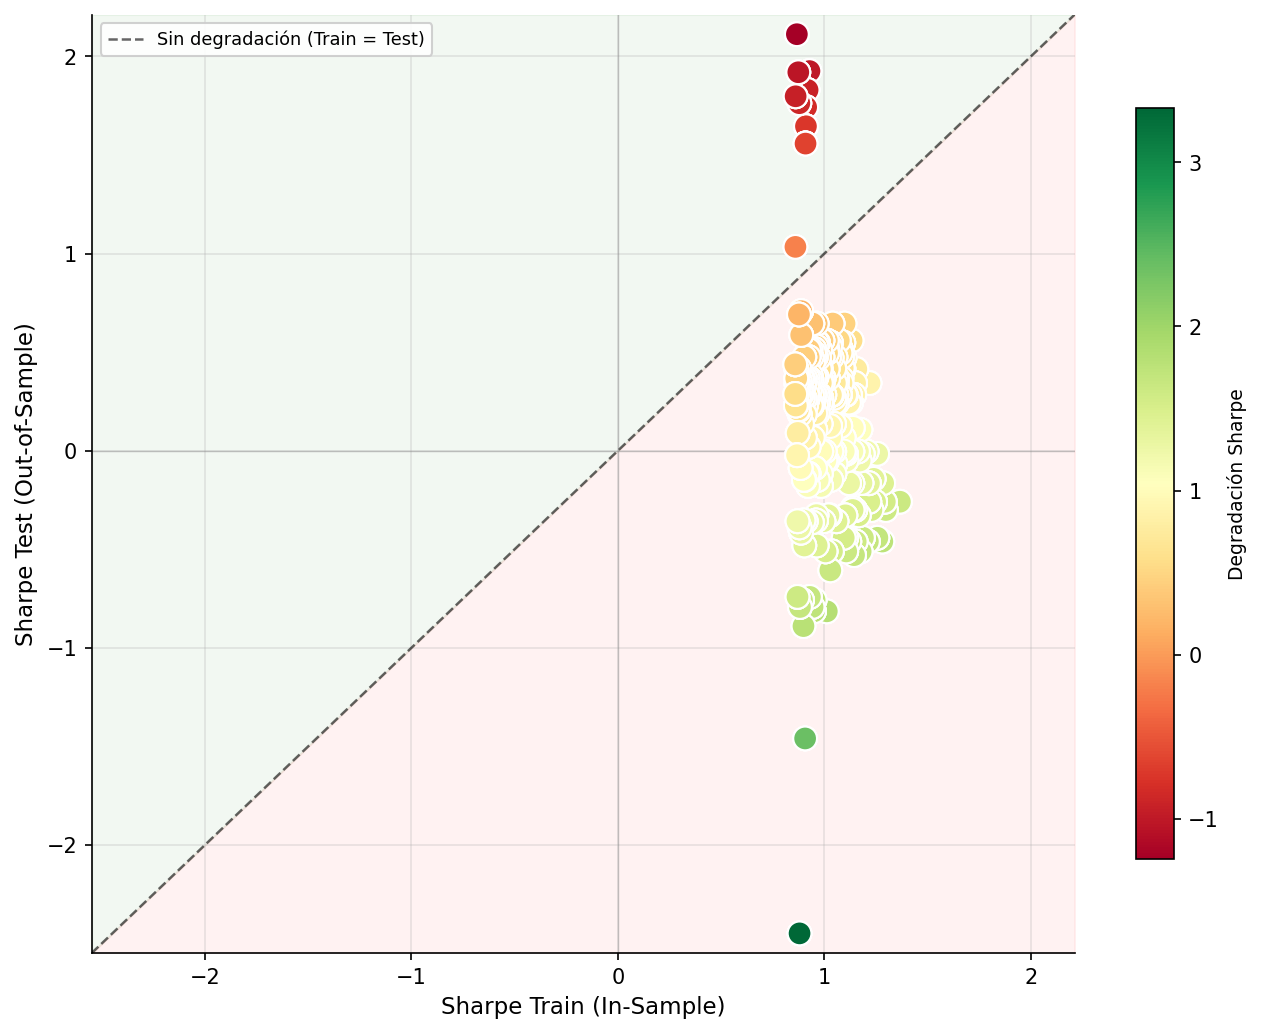
\includegraphics[width=0.8\textwidth]{media/wf_03_sharpe_scatter.png}
    \caption{Dispersión Sharpe Train vs.\ Sharpe Test. Cada punto
    representa una configuración. El color codifica la magnitud
    de la degradación (verde: baja, rojo: alta).
    Fuente: Elaboración propia.}
    \label{fig:sharpe_scatter}
\end{figure}

Se observa un fenómeno relevante: la configuración
con mejor Sharpe en entrenamiento (1,366) se sitúa en la zona
inferior del gráfico, con un Sharpe en prueba de \(-0,259\). Es
decir, la mejor estrategia aparente es, precisamente, la que más
fracasa al enfrentarse a datos nuevos. Este resultado constituye
una demostración de sobreajuste y muestra la
necesidad de la validación con datos no vistos.

Por el contrario, las configuraciones que mejores resultados
obtienen en Test no son las que lideraban el ranking en
entrenamiento. Esto refleja la existencia de
estrategias que, sin alcanzar los valores extremos de Sharpe en
la muestra de entrenamiento, poseen una estructura menos
sensible al ruido del periodo histórico.

\paragraph{Análisis de la degradación por ranking}

La Figura~\ref{fig:degradation_bar} muestra las barras
comparativas del ratio de Sharpe en entrenamiento y en prueba
para las configuraciones extremas del ranking. Se han
seleccionado las 15 configuraciones con menor Sharpe de
entrenamiento y las 15 con mayor Sharpe de entrenamiento.

\begin{figure}[H]
    \centering
    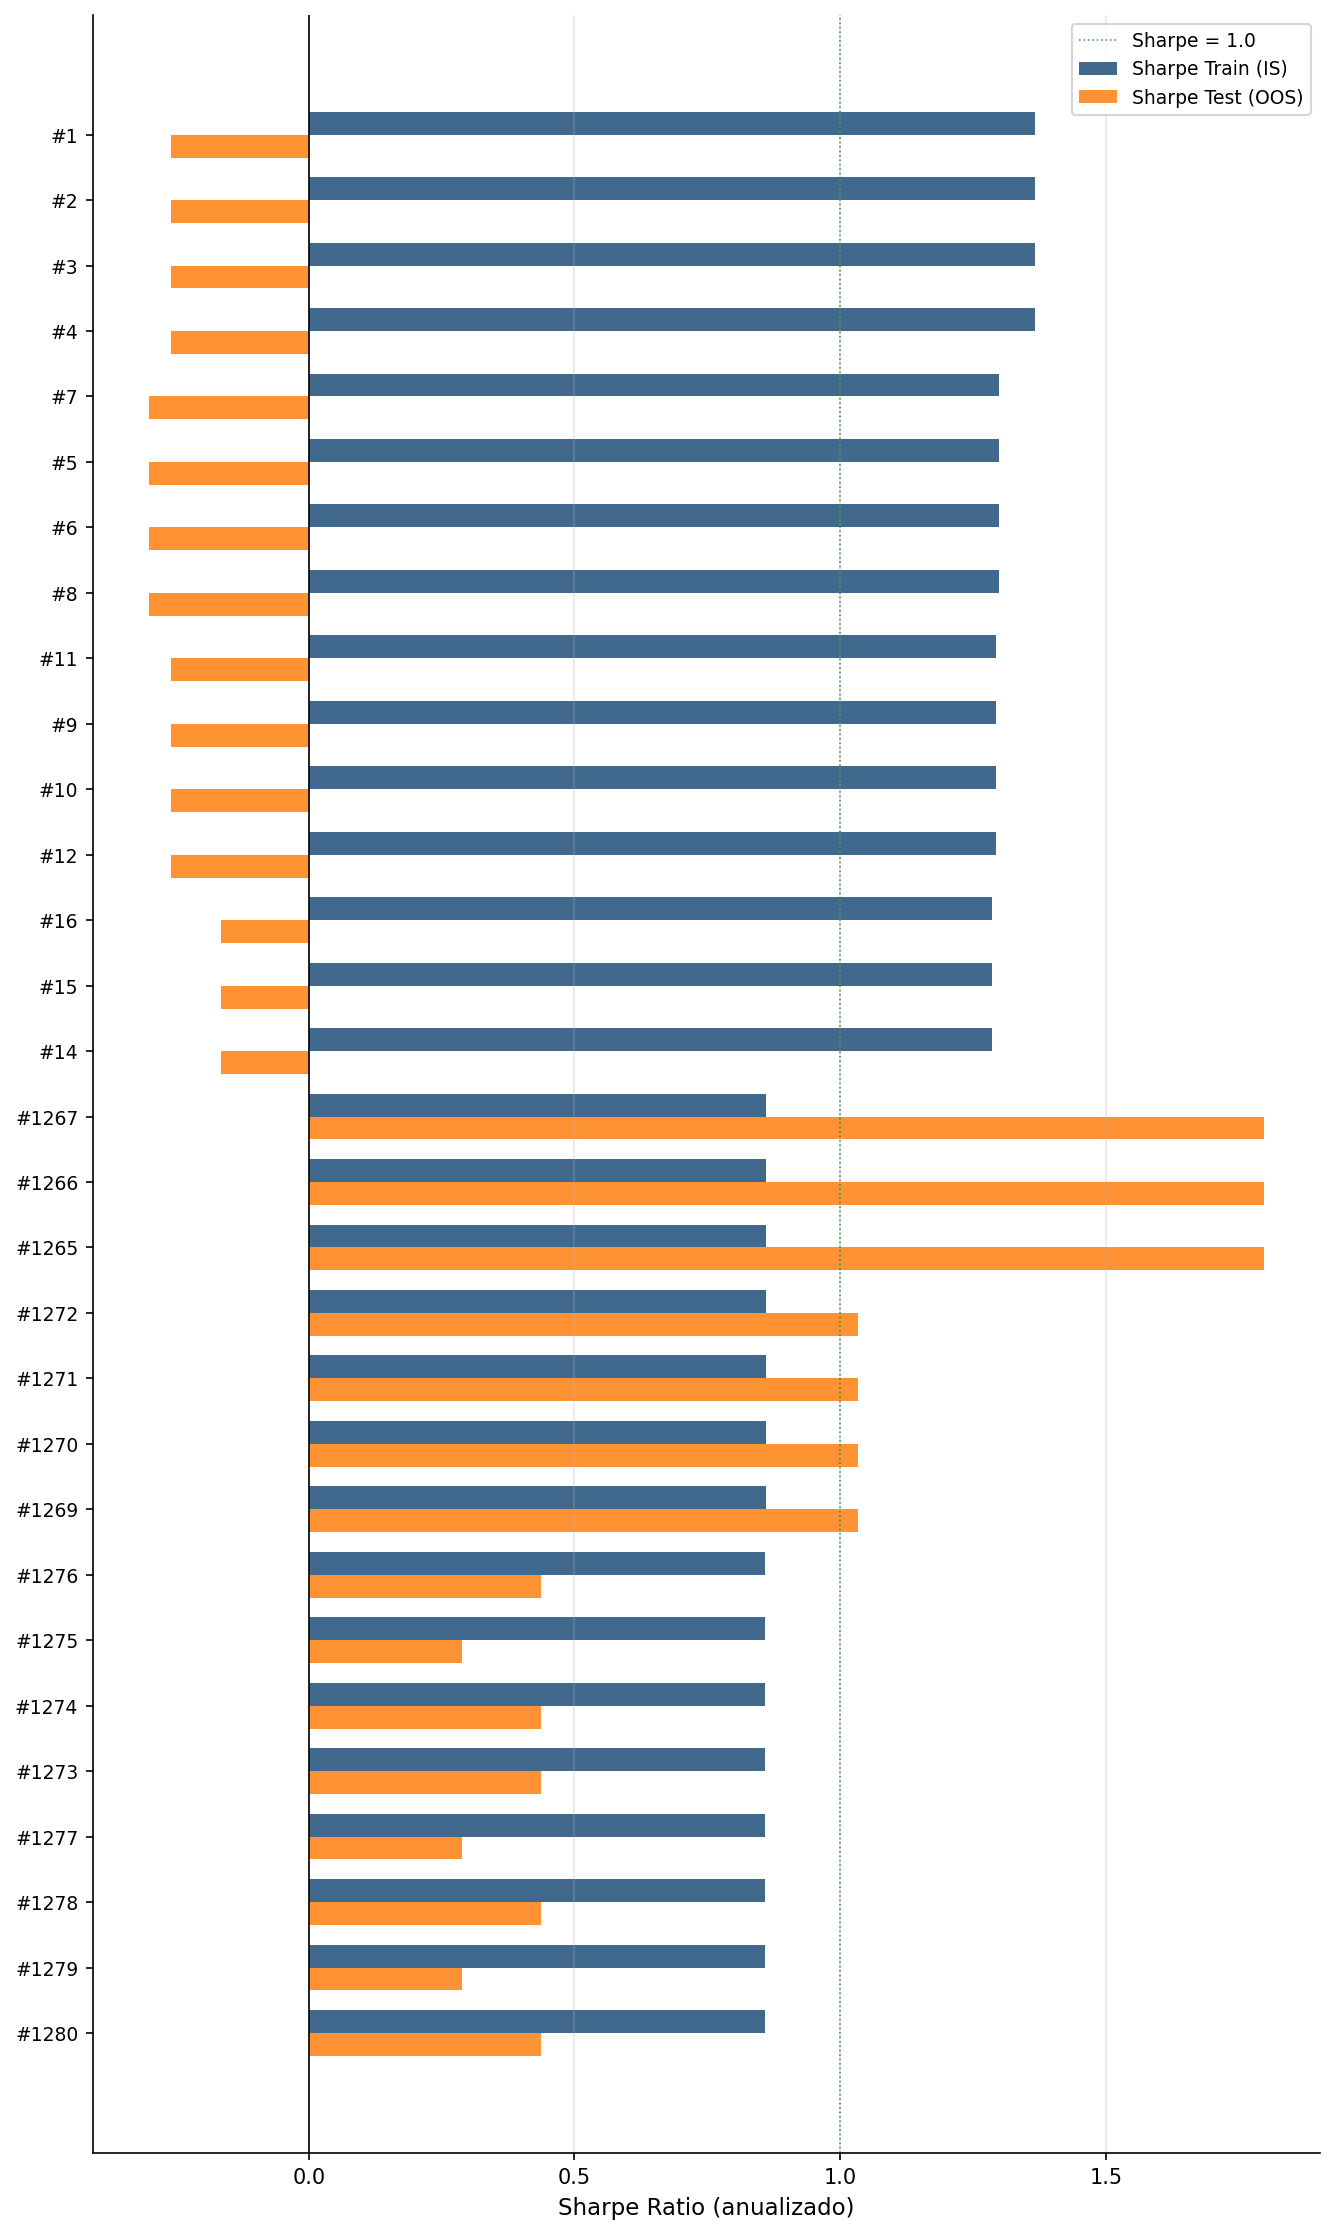
\includegraphics[width=0.85\textwidth]{media/wf_05_degradation_bar.png}
    \caption{Comparación del Sharpe en Train (azul) y en
    Test (naranja) para las configuraciones extremas. Se observa
    que las configuraciones con mayor Sharpe en entrenamiento
    presentan una degradación más elevada. Fuente: Elaboración propia.}
    \label{fig:degradation_bar}
\end{figure}

Se observa que las configuraciones con Sharpe de
entrenamiento más elevados muestran una caída
mayor en la ventana de Test. Este comportamiento refuerza la
necesidad de no confiar exclusivamente en las métricas de
entrenamiento para la selección del modelo final.

Por el contrario, las configuraciones con Sharpe de entrenamiento
moderado (en torno a 0,8--1,0) presentan, en muchos casos, una
degradación menor o incluso nula, lo que sugiere que estas
estrategias poseen una estructura más robusta.

\paragraph{Identificación de la mejor configuración global}

Se identifican las
configuraciones con mejor rendimiento en la ventana de prueba.
La Tabla~\ref{tab:top10_oos} presenta las diez estrategias con
Sharpe más elevado en datos no vistos.

\begin{table}[H]
\centering
\small
\begin{tabular}{clccccrr}
\toprule
\textbf{\#} & \textbf{Señal} & \textbf{Cl.} & \textbf{Freq.} & \textbf{Top} &
\textbf{RW} & \textbf{Sharpe\_Test} & \textbf{CAGR (\%)} \\
\midrule
1  & ALR1M\_Z    & 1 & M  & 8  & No  & \textbf{2,113} & 28,47 \\
2  & ALR1W\_Z    & 4 & M  & 3  & Sí  & 1,926         & 13,63 \\
3  & ALR1W\_Z    & 1 & M  & 10 & No  & 1,920         & 22,14 \\
4  & ALR1W\_Z    & 4 & M  & 4  & Sí  & 1,830         & 16,74 \\
5  & ALR1W\_Z    & 4 & M  & 5  & Sí  & 1,798         & 17,95 \\
6  & ALR1W\_Z    & 1 & M  & 10 & Sí  & 1,763         & 22,13 \\
7  & ALR1W\_Z    & 4 & M  & 2  & Sí  & 1,743         & 6,32  \\
8  & ALR1W\_Z    & 3 & Q  & 1  & No  & 1,646         & 16,72 \\
9  & ALR1W\_Z    & 3 & Q  & 1  & Sí  & 1,646         & 16,72 \\
10 & ALR1W\_Z    & 4 & M  & 3  & No  & 1,559         & 19,01 \\
\bottomrule
\end{tabular}
\caption{Top 10 configuraciones por Sharpe en Test.
Fuente: Elaboración propia.}
\label{tab:top10_oos}
\begin{flushleft}
\small \textit{Nota:} \textbf{Cl.}=active\_cluster,
\textbf{Freq.}=rebalance\_freq, \textbf{RW}=rank\_weighted.
\end{flushleft}
\end{table}

La mejor configuración global alcanza un ratio de Sharpe en
Test de 2,113, correspondiente a la señal \texttt{ALR1M\_Z}
(momento a un mes) sobre el clúster 1 (Bear market rally) con
rebalanceo mensual y tamaño de cartera \texttt{top\_n=8}. No
obstante, debe señalarse que este valor excepcional puede estar
influido por las condiciones específicas del periodo de prueba.

Las nueve configuraciones restantes del Top 10 comparten la
señal \texttt{ALR1W\_Z} (momento a una semana), lo que indica
que las señales de corto plazo son las que mejor se adaptan a
las condiciones del periodo de prueba. Destaca la diversidad
de regímenes representados: el clúster 4 (Estrés/Capitulación)
aparece en cinco configuraciones, el clúster 1 (Bear market
rally) en tres y el clúster 3 (Pullback alcista) en dos. El
rebalanceo mensual es mayoritario (ocho de diez), mientras que
la ponderación por ranking y la equiponderada se reparten al
50\,\%.

La configuración que ofrece el mejor equilibrio entre Sharpe
y rentabilidad dentro del grupo \texttt{ALR1W\_Z} es la que
combina el clúster 1 con \texttt{top\_n=10} y ponderación
equiponderada, alcanzando un Sharpe en Test de 1,920 y una
CAGR del 22,14\,\%.

\paragraph{Curva de capital de la configuración ganadora}

La Figura~\ref{fig:equity_winner} muestra la evolución del
capital acumulado de la mejor configuración en Test,
expresada en términos de mark-to-market diario real, frente al
índice de referencia SPY. La línea vertical punteada marca la
separación entre la ventana de entrenamiento y la ventana de
prueba.

\begin{figure}[H]
    \centering
    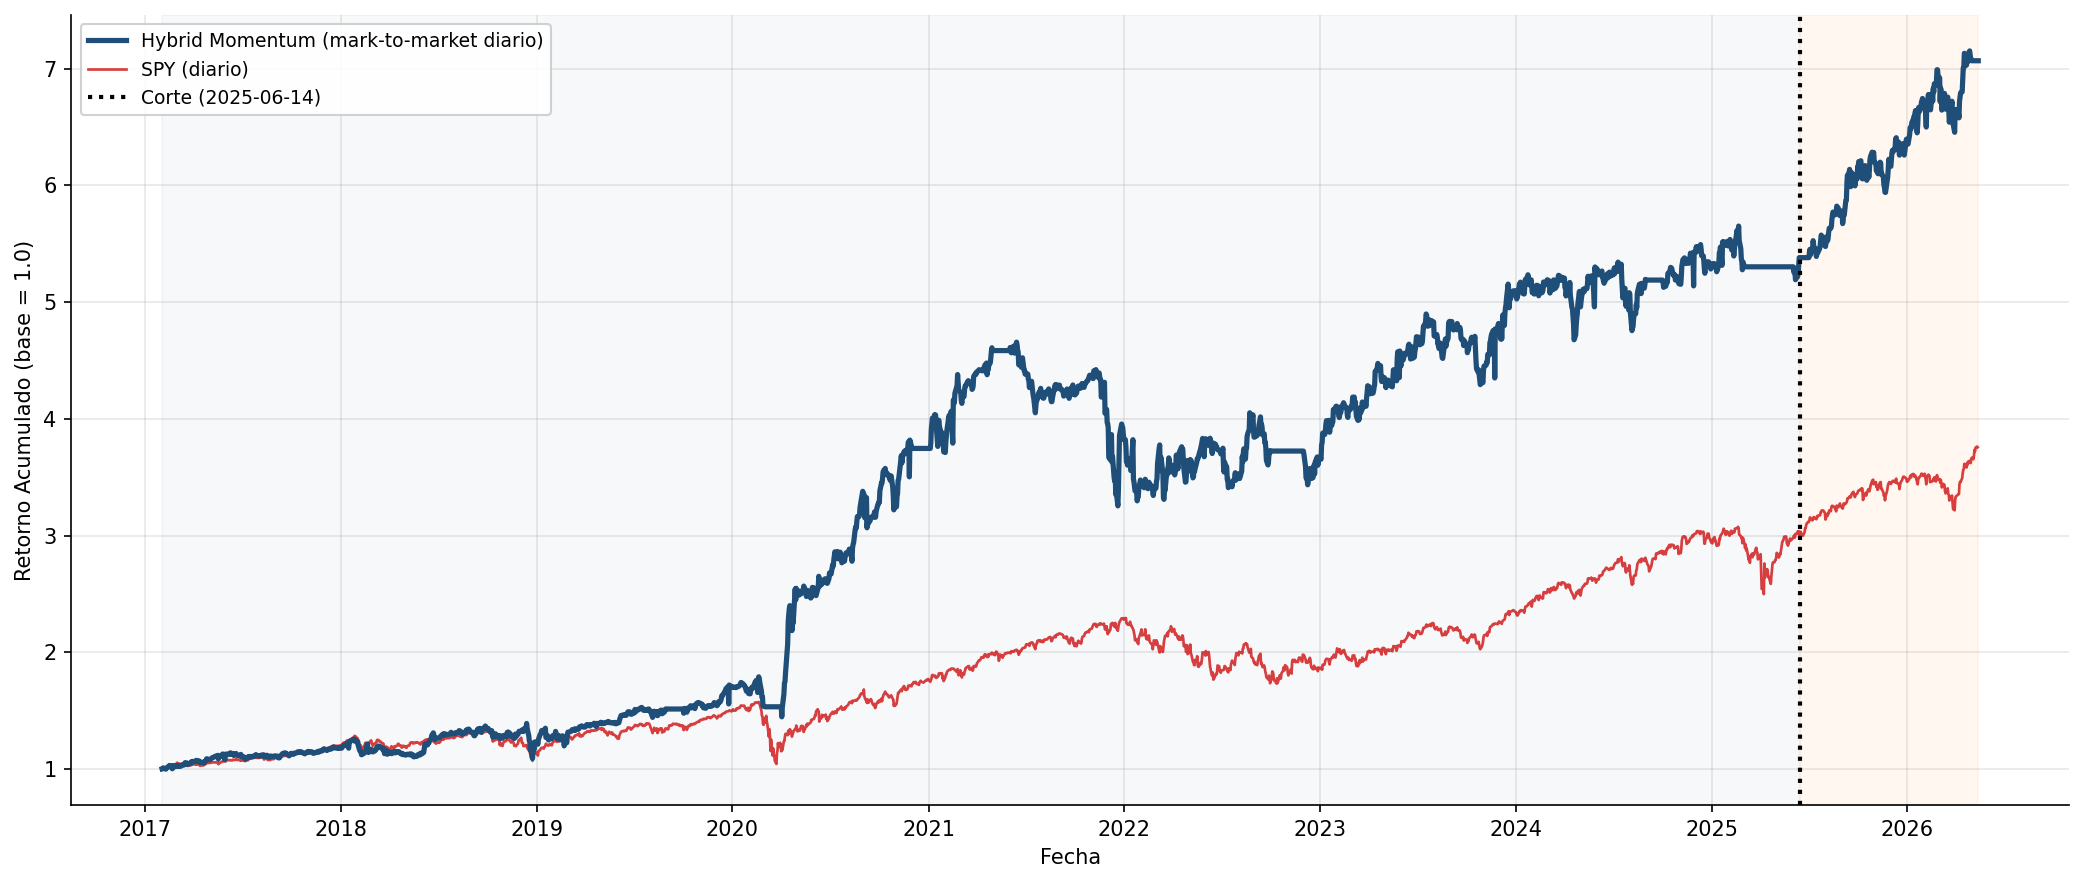
\includegraphics[width=\textwidth]{media/wf_01_equity_curve_winner_daily.png}
    \caption{Curva de capital de la mejor configuración
    en Test con resolución diaria frente al benchmark SPY.
    La línea vertical indica el inicio de la ventana de prueba.
    Fuente: Elaboración propia.}
    \label{fig:equity_winner}
\end{figure}

Se aprecia que la estrategia mantiene una trayectoria
ascendente consistente durante todo el periodo analizado,
acumulando una rentabilidad superior a la del
índice de referencia. La pendiente sostenida de la curva,
especialmente durante la ventana de prueba, sugiere que el
sistema es capaz de extraer señales de valor añadido de forma
consistente.

\paragraph{Comparativa con el índice de referencia SPY}

La Tabla~\ref{tab:comparativa_spy} presenta una comparación
entre las métricas de la mejor configuración
en Test y las del índice de referencia SPY.

\begin{table}[H]
\centering
\begin{tabular}{lrrr}
\toprule
\textbf{Métrica} & \textbf{Estrategia} & \textbf{SPY} \\
\midrule
Sharpe                & 2,113 & 0,585 \\
CAGR (\%)             & 28,47 & 12,10 \\
Caída máxima (\%)     & -4,05 & -12,10 \\
\bottomrule
\end{tabular}
\caption{Comparativa de la mejor configuración en Test frente al
benchmark SPY. Fuente: Elaboración propia.}
\label{tab:comparativa_spy}
\end{table}

La estrategia triplica prácticamente el ratio de Sharpe
del índice de referencia (2,113 frente a 0,585) y más que duplica
la rentabilidad anualizada (28,47\,\% frente a 12,10\,\%),
con una caída máxima notablemente inferior (-4,05\,\% frente a
-12,10\,\%). El sistema propuesto es capaz de generar
\textit{alpha} sobre el mercado de referencia.


\paragraph{Selección del modelo final}

Del análisis anterior se identifica como configuración de
referencia la estrategia \textbf{ALR1M\_Z} sobre el clúster 1
(Bear market rally), con rebalanceo mensual,
\texttt{top\_n=8} y ponderación equiponderada.

El criterio que justifica esta selección es:

\begin{itemize}
    \item \textbf{Rendimiento superior.} La estrategia triplica el
    Sharpe del índice de referencia (2,113 frente a 0,585) y más
    que duplica la rentabilidad anualizada (28,47\,\% frente a
    12,10\,\%), con una caída máxima de solo -4,05\,\% frente al
    -12,10\,\% del SPY.

    
\end{itemize}

No obstante, debe señalarse que este resultado excepcional
podría estar influido por las condiciones específicas del
periodo de prueba. Como alternativa más conservadora, las
configuraciones basadas en \texttt{ALR1W\_Z} ofrecen un
respaldo estadístico más amplio al concentrar nueve de las
diez posiciones del Top 10.

Los parámetros completos se resumen en la
Tabla~\ref{tab:modelo_final}.

\begin{table}[H]
\centering
\small
\begin{tabular}{ll}
\toprule
\textbf{Parámetro} & \textbf{Valor} \\
\midrule
Señal de momentum    & ALR1M\_Z (1 mes) \\
Clúster              & 1 (Bear market rally) \\
Rebalanceo           & Mensual (M) \\
Tamaño de cartera    & \texttt{top\_n=8} (8 activos) \\
Ponderación          & Equiponderada \\
Ventana anomalías    & 1 día \\
Tamaño mínimo cartera& 1 (sin mínimo exigido) \\
\bottomrule
\end{tabular}
\caption{Parámetros del modelo final seleccionado.
Fuente: Elaboración propia.}
\label{tab:modelo_final}
\end{table}


\subsubsection{Análisis de Robustez}

Esta sección aborda la cuestión de si los resultados obtenidos
pueden considerarse estadísticamente fiables o si, por el
contrario, responden a patrones 'falsos' propios del periodo de
evaluación.

\paragraph{Importancia de los hiperparámetros}

Para determinar qué parámetros del sistema ejercen una influencia
determinante sobre el rendimiento fuera de muestra, se ha
entrenado un modelo de bosque aleatorio (\textit{Random Forest})
con 300 árboles para predecir el Sharpe en prueba a partir de los
hiperparámetros de cada configuración. La
Tabla~\ref{tab:feature_importance} presenta la importancia
relativa de cada variable en la predicción.

\begin{table}[H]
\centering
\begin{tabular}{lr}
\toprule
\textbf{Variable} & \textbf{Importancia (\%)} \\
\midrule
top\_n                   & 25,99 \\
min\_portfolio\_size     & 23,64 \\
active\_cluster          & 21,01 \\
momentum\_signal         & 20,12 \\
rebalance\_freq          & 6,02  \\
rank\_weighted           & 3,22  \\
anomaly\_lookback\_days  & 0,01  \\
\bottomrule
\end{tabular}
\caption{Importancia de los hiperparámetros en la predicción del
Sharpe en Test mediante Random Forest. Fuente: Elaboración propia.}
\label{tab:feature_importance}
\end{table}

Los resultados revelan que los tres parámetros con mayor impacto
son \texttt{top\_n} (tamaño de la cartera), \texttt{min\_portfolio\_size}
(tamaño mínimo para evitar periodos en efectivo) y
\texttt{active\_cluster} (régimen de mercado seleccionado), que
conjuntamente explican más del 70\,\% de la varianza del
rendimiento fuera de muestra. La señal de momentum contribuye
con un 20\,\% adicional.

Resulta especialmente relevante la contribución prácticamente
nula del parámetro \texttt{anomaly\_lookback\_days} (ventana de
retrospectiva para el filtro DBSCAN). Este hallazgo sugiere que
la presencia del filtro topológico es importante para la
integridad del sistema, pero la longitud de la ventana de
observación de anomalías no es un factor determinante del
rendimiento, probablemente porque el filtro diario \textit{cross-
sectional} de DBSCAN proporciona una protección suficientemente
robusta con independencia del horizonte retrospectivo concreto
utilizado.

\paragraph{Sensibilidad de parámetros en ventana de prueba}

La Figura~\ref{fig:oos_sensitivity} descompone el rendimiento en Test agregado de las 1.064 configuraciones con Sharpe
de prueba válido, agrupándolas por el valor de cada
hiperparámetro. Para cada parámetro, se reconstruye la curva de
capital diaria de todas las configuraciones que comparten ese
valor y se promedia, permitiendo aislar visualmente el efecto
marginal de cada variable sobre el rendimiento conjunto.

\begin{figure}[H]
    \centering
    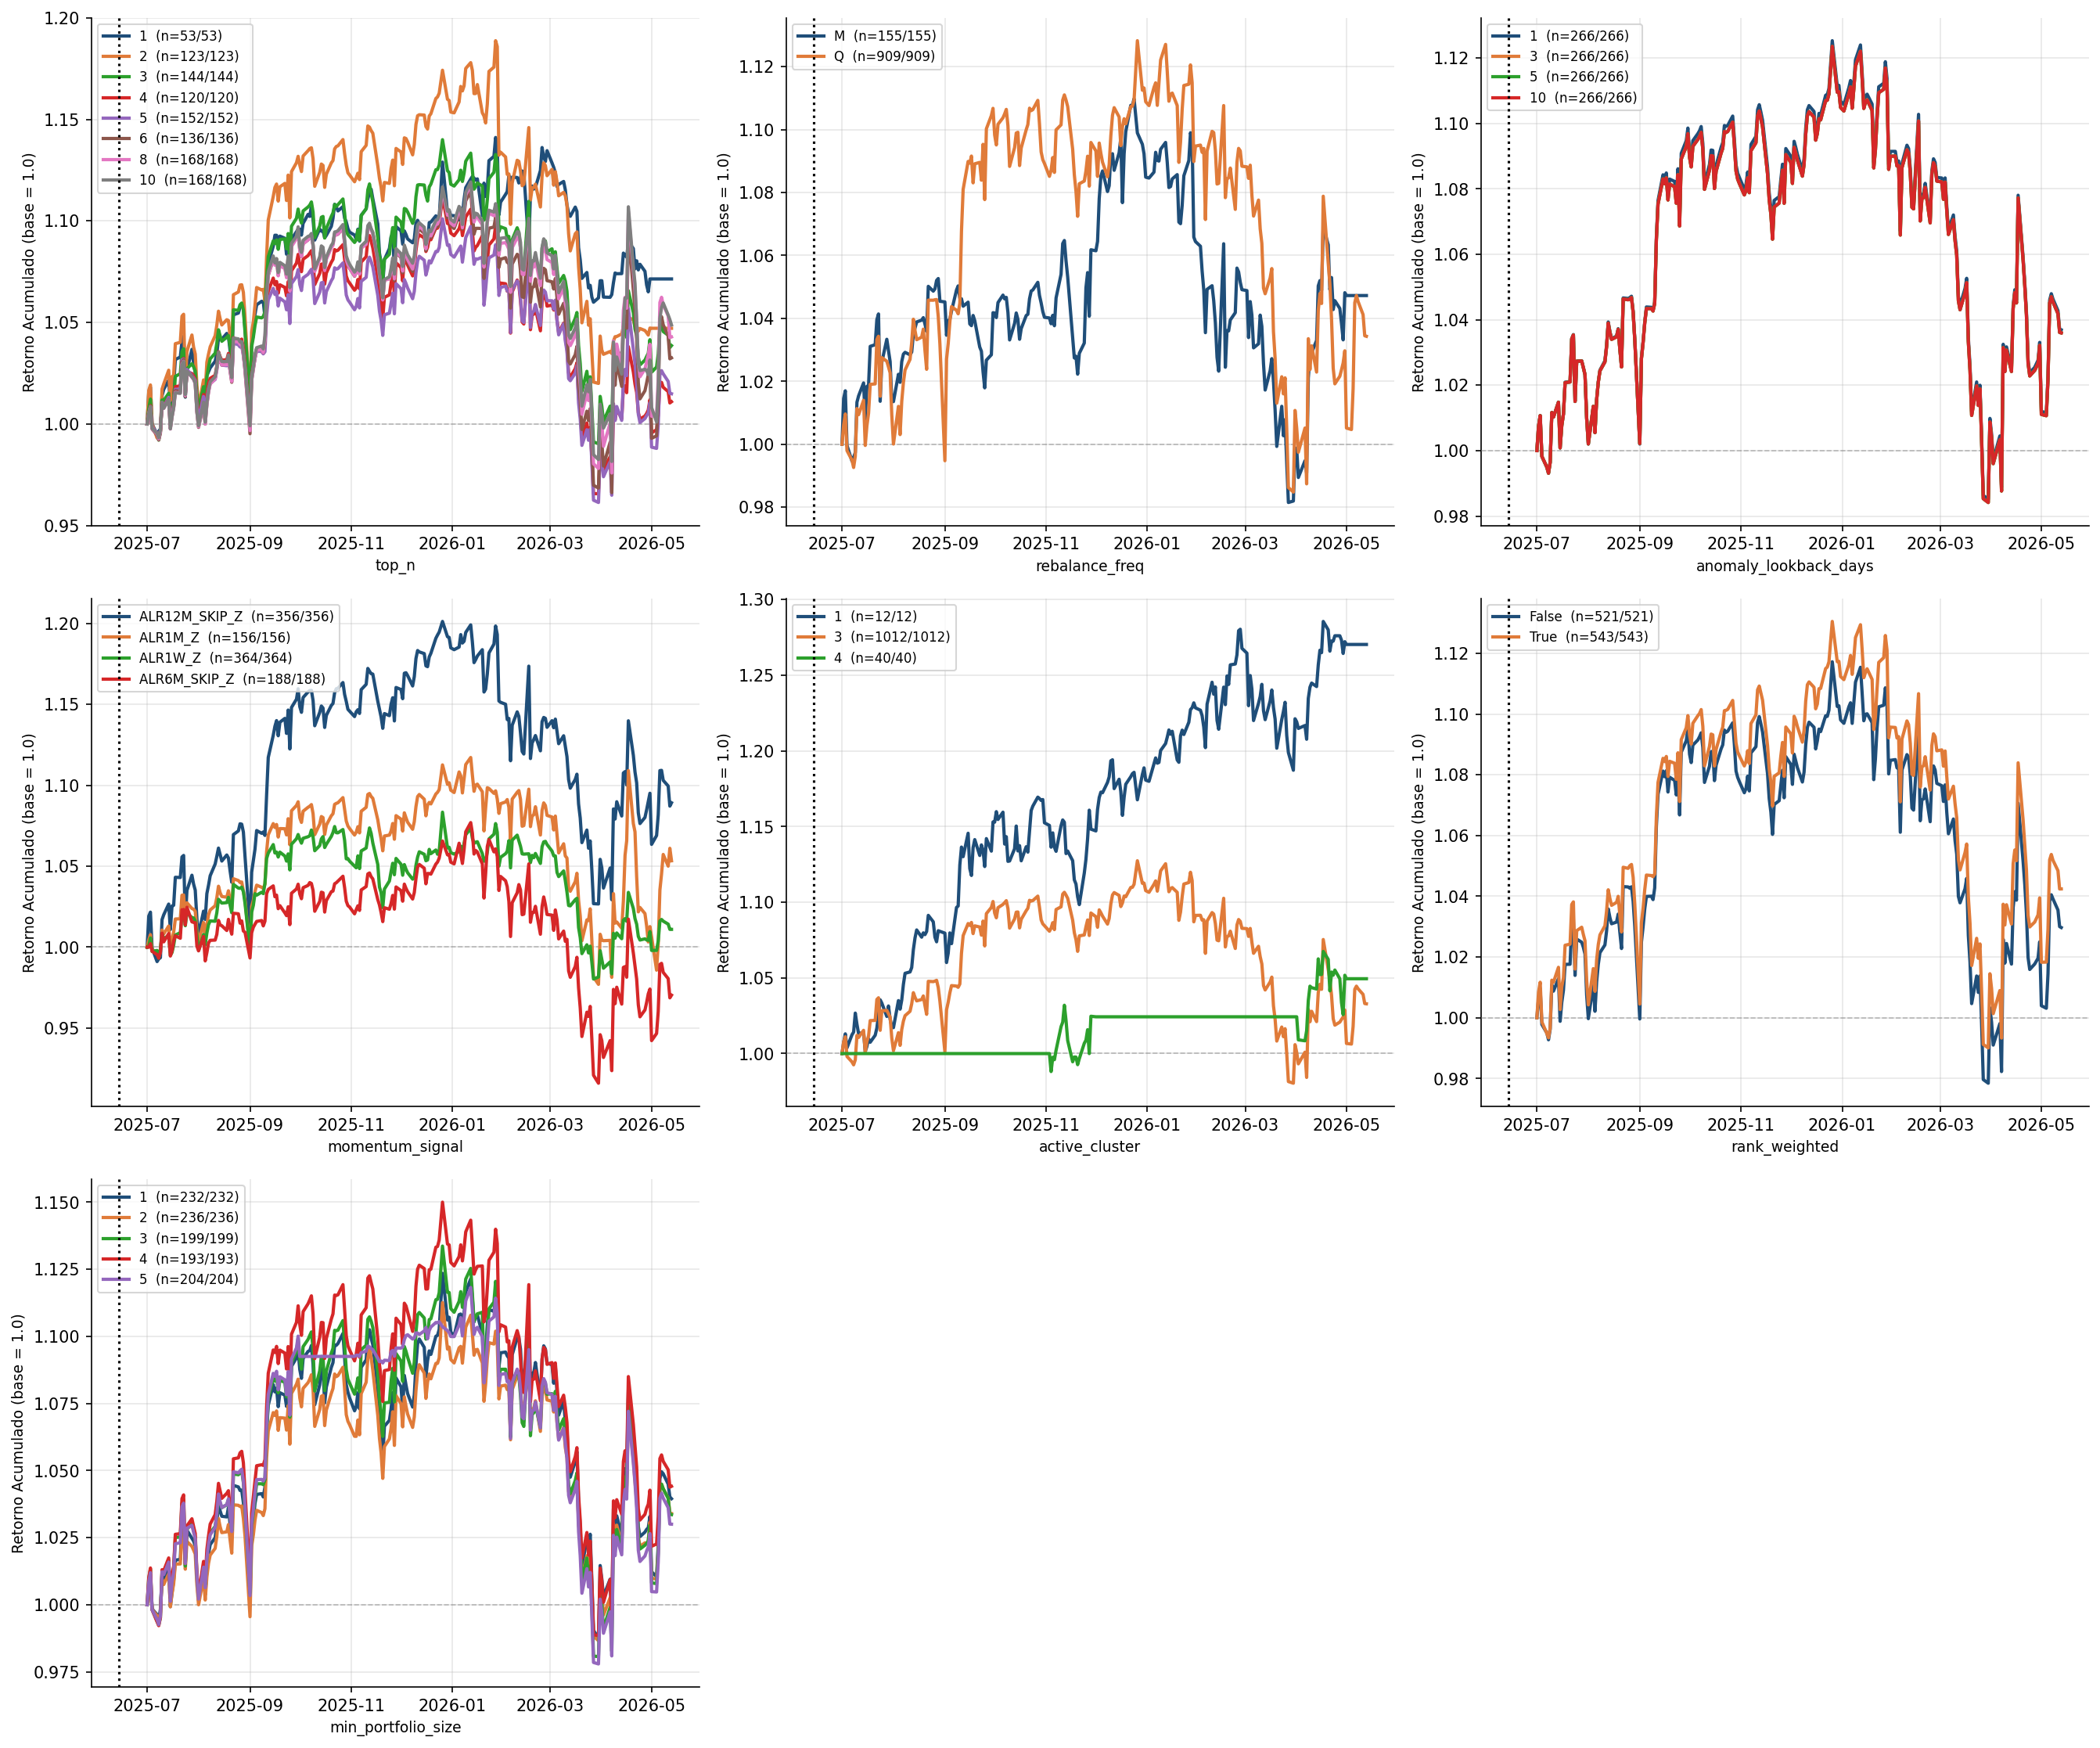
\includegraphics[width=1.05\textwidth]{media/wf_07_oos_parameter_sensitivity.png}
    \caption{Curvas de capital medias Out-of-Sample agrupadas por
    valor de hiperparámetro. Cada panel desagrega el efecto de
    una variable sobre el rendimiento agregado del conjunto de
    configuraciones (\textit{N}=1.064). Fuente: Elaboración propia.}
    \label{fig:oos_sensitivity}
\end{figure}

Se observa que:
\begin{itemize}
    
    \item \textbf{active\_cluster}: el clúster 1 es el que
    presenta el rendimiento acumulado medio más elevado (final
    de 1,270), seguido del clúster 4 (1,050). El clúster 3,
    pese a concentrar el 95\,\% de las configuraciones,
    muestra la curva media más baja (1,033).
    
    \item \textbf{rebalance\_freq}: la frecuencia mensual
    (\texttt{M}) supera a la trimestral en rendimiento acumulado
    medio (1,047 frente a 1,034), pese a que esta última
    concentra el 85\,\% de las configuraciones.
    \item \textbf{rank\_weighted}: la ponderación por ranking
    ofrece un rendimiento ligeramente superior a la
    equiponderada (1,042 frente a 1,030), aunque la diferencia
    es muy leve y ambas opciones generan rentabilidad positiva
    en promedio.
\end{itemize}

\paragraph{Conclusiones del capítulo}

Los resultados presentados a lo largo de este capítulo permiten
extraer las siguientes conclusiones consolidadas:

\begin{enumerate}
    \item \textbf{El sobreajuste existe y es significativo.} La
    mejor configuración en entrenamiento (Sharpe 1,366) presenta
    un rendimiento negativo en la ventana de prueba (\(-0,259\)).
    Este fenómeno es común a cualquier proceso de optimización
    sobre datos históricos y debe ser gestionado mediante
    validación con datos no vistos.

    \item \textbf{La robustez existe y es identificable.} El
    55,9\,\% de las configuraciones mantienen un Sharpe positivo
    en prueba, y la mejor de ellas alcanza un valor de 2,113
    (señal \texttt{ALR1M\_Z} sobre clúster 1, rebalanceo mensual,
    \texttt{top\_n=8}). Esta configuración se consolida como el
    modelo de referencia del sistema.

    \item \textbf{El sistema supera al benchmark de referencia.}
    Tanto en términos de Sharpe (2,113 frente a 0,585) como de
    CAGR (28,47\,\% frente a 12,10\,\%), la mejor configuración
    en Test triplica el rendimiento ajustado al riesgo del
    índice SPY, con una caída máxima notablemente inferior.

    \item \textbf{La selección del régimen de mercado es
    crítica.} El parámetro \texttt{active\_cluster} explica el
    21\,\% de la varianza del rendimiento fuera de muestra. El
    clúster 3 (Pullback alcista) se consolida como el régimen
    más favorable para estrategias basadas en momentum.

    \item \textbf{El filtro topológico DBSCAN es un componente
    estructural, no una variable de ajuste.} La ventana de
    retrospectiva para la detección de anomalías (\texttt{anomaly\_lookback\_days})
    presenta una importancia prácticamente nula en el modelo de
    predicción, lo que sugiere que la presencia del filtro DBSCAN proporciona una protección
    suficiente contra el ruido.
\end{enumerate}

A la vista de estos resultados, el modelo seleccionado como
configuración de referencia es la estrategia
\texttt{ALR1M\_Z} sobre el clúster 1, con rebalanceo
mensual, \texttt{top\_n=8} y ponderación equiponderada.
Esta configuración ofrece la mayor rentabilidad, superando
al índice de referencia SPY tanto en términos
de Sharpe como de rentabilidad anualizada.


\endinput

% =============================================================================

\subsection{Evaluación y Backtesting}

En este capítulo se describe la evaluación
diseñada para validar el modelo propuesto, se presentan
los resultados obtenidos tanto en la fase de
entrenamiento (Train) como en la fase de prueba
(Test) y se analiza la robustez de las
configuraciones analizadas. El objetivo fundamental es
determinar si la arquitectura DBSCAN + K-Means,
combinada con una selección dinámica por momentum, es capaz de
generar rentabilidades (teniendo en cuenta el riesgo) superiores a las de
un índice de referencia.

A lo largo del capítulo se analiza si existe una combinación de hiperparámetros que responda de forma estable a datos no vistos, se cuantifica la magnitud de la degradación por sobreajuste al seleccionar las mejores configuraciones en la muestra de entrenamiento, y se identifican los parámetros que tienen una influencia sobre el rendimiento en test.


\subsubsection{Sistema de Evaluación}

La validación del sistema se ha diseñado con el objetivo de
aproximar, en la medida de lo posible, un entorno real de
inversión. Para ello, se establecen una serie de criterios orientados a evitar sesgos y a garantizar que la
comparación entre estrategias sea homogénea.

\paragraph{Causalidad temporal ($T/T+1$)}

Las decisiones de inversión se generan únicamente con la
información disponible al cierre del último día hábil del período
de rebalanceo $T$. La entrada efectiva en cartera se realiza al
cierre del primer día hábil posterior ($T+1$). De esta forma,
se evita incorporar información futura en el proceso de decisión.

Los retornos de cada cartera se calculan desde el cierre de
$T+1$ hasta el cierre del siguiente período de rebalanceo.
Además, todas las transformaciones estadísticas utilizadas por
el modelo se estiman
exclusivamente con datos históricos disponibles en cada fecha
según la Ecuación~\ref{eq:zscore_rolling}.

\paragraph{Ventanas temporales y división Train/Test}

El periodo completo de análisis comprende desde enero de 2017
hasta la fecha más reciente disponible. Para garantizar la
independencia entre la fase de optimización y la fase de
validación, se establece un punto de corte dinámico situado
exactamente un año antes del momento de ejecución del
experimento:

\begin{itemize}
    \item \textbf{Ventana de entrenamiento (Train):}
    desde enero de 2017 hasta un año antes de la fecha actual.
    Sobre esta ventana se ejecuta el \textit{grid search}.
    \item \textbf{Ventana de prueba (Test):}
    desde la fecha de corte hasta la actualidad. Sobre esta
    ventana se evalúan exclusivamente las configuraciones
    seleccionadas en la fase de entrenamiento, sin ningún tipo
    de realimentación hacia el modelo.
\end{itemize}

\paragraph{Benchmark de referencia}

Como índice de comparación se utiliza el ETF \textit{SPDR
S\&P 500 ETF Trust} (SPY), ampliamente empleado como referencia de la renta variable estadounidense. Su curva de
capital se normaliza a base 1,0 en la misma fecha inicial que la
estrategia.

\paragraph{Arquitectura del proceso experimental}

El diseño sigue dos etapas diferenciadas, ilustrado en la
Figura~\ref{fig:experimental_design}:

\begin{enumerate}
    \item \textbf{Búsqueda en malla (\textit{Grid Search})
    con datos de entrenamiento}: Se enumeran las 12.800
    combinaciones resultantes de los
    siete hiperparámetros definidos en el sistema
    (\texttt{top\_n}, \texttt{rebalance\_freq},
    \texttt{anomaly\_lookback\_days}, \texttt{momentum\_signal},
    \texttt{active\_cluster}, \texttt{rank\_weighted} y
    \texttt{min\_portfolio\_size}). Cada combinación se evalúa
    sobre la ventana de entrenamiento y se registran sus
    métricas.

    \item \textbf{Validación con datos de prueba}: Se
    selecciona el 10\,\% de las configuraciones con mejor
    \textit{ratio de Sharpe} en la fase anterior (1.280 estrategias). Cada una de ellas se re-evalúa sobre la
    ventana de Test, cronológicamente posterior y nunca vista
    durante la optimización. Se mide la degradación del Sharpe
    como diferencia entre el valor en entrenamiento y en prueba,
    siendo la métrica central de sobreajuste.
\end{enumerate}

\begin{figure}[H]
    \centering
    \begin{tikzpicture}[node distance=1.5cm, auto,
        block/.style={rectangle, draw, text width=7cm,
        text centered, rounded corners, minimum height=0.8cm,
        font=\small},
        arrow/.style={draw, -latex', thick}]

        \node [block, fill=green!10] (grid)
            {Grid Search \\
             7 parámetros $\times$ 12.800 combinaciones \\
             Ventana: 2017 -- ($t-1$ año)};
        \node [block, below of=grid, fill=yellow!15] (top)
            {Selección Top 10\,\% por Sharpe \\
             $\approx$ 1.280 configuraciones \\};
        \node [block, below of=top, fill=cyan!15] (wf)
            {Evaluación en datos de prueba \\
             Ventana: ($t-1$ año) -- ($t$) \\
             Sharpe\_Test, Degradación};
        \node [block, below of=wf, fill=orange!15] (analysis)
            {Análisis de Robustez \\
             Importancia de parámetros, \\
             Sensibilidad, Comparativa vs SPY};

        \path [arrow] (grid) -- (top);
        \path [arrow] (top) -- (wf);
        \path [arrow] (wf) -- (analysis);
    \end{tikzpicture}
    \caption{Arquitectura del proceso experimental. Fuente: Elaboración propia.}
    \label{fig:experimental_design}
\end{figure}


\subsubsection{Búsqueda en malla (Grid Search) en datos de entrenamiento}

Sobre la ventana de entrenamiento se ejecuta un barrido de las 12.800 combinaciones de hiperparámetros
ya mencionadas. Todas las combinaciones
generaron resultados válidos.

\paragraph{Distribución del ratio de Sharpe en entrenamiento}

La Figura~\ref{fig:hyperparam_dist} muestra la distribución de
los siete hiperparámetros dentro del subconjunto de estrategias
que pertenecen al 10\,\% superior en Sharpe dentro de la muestra
de entrenamiento. Este análisis permite identificar qué valores
de cada parámetro aparecen con mayor frecuencia entre las mejores
configuraciones.

\begin{figure}[H]
    \centering
    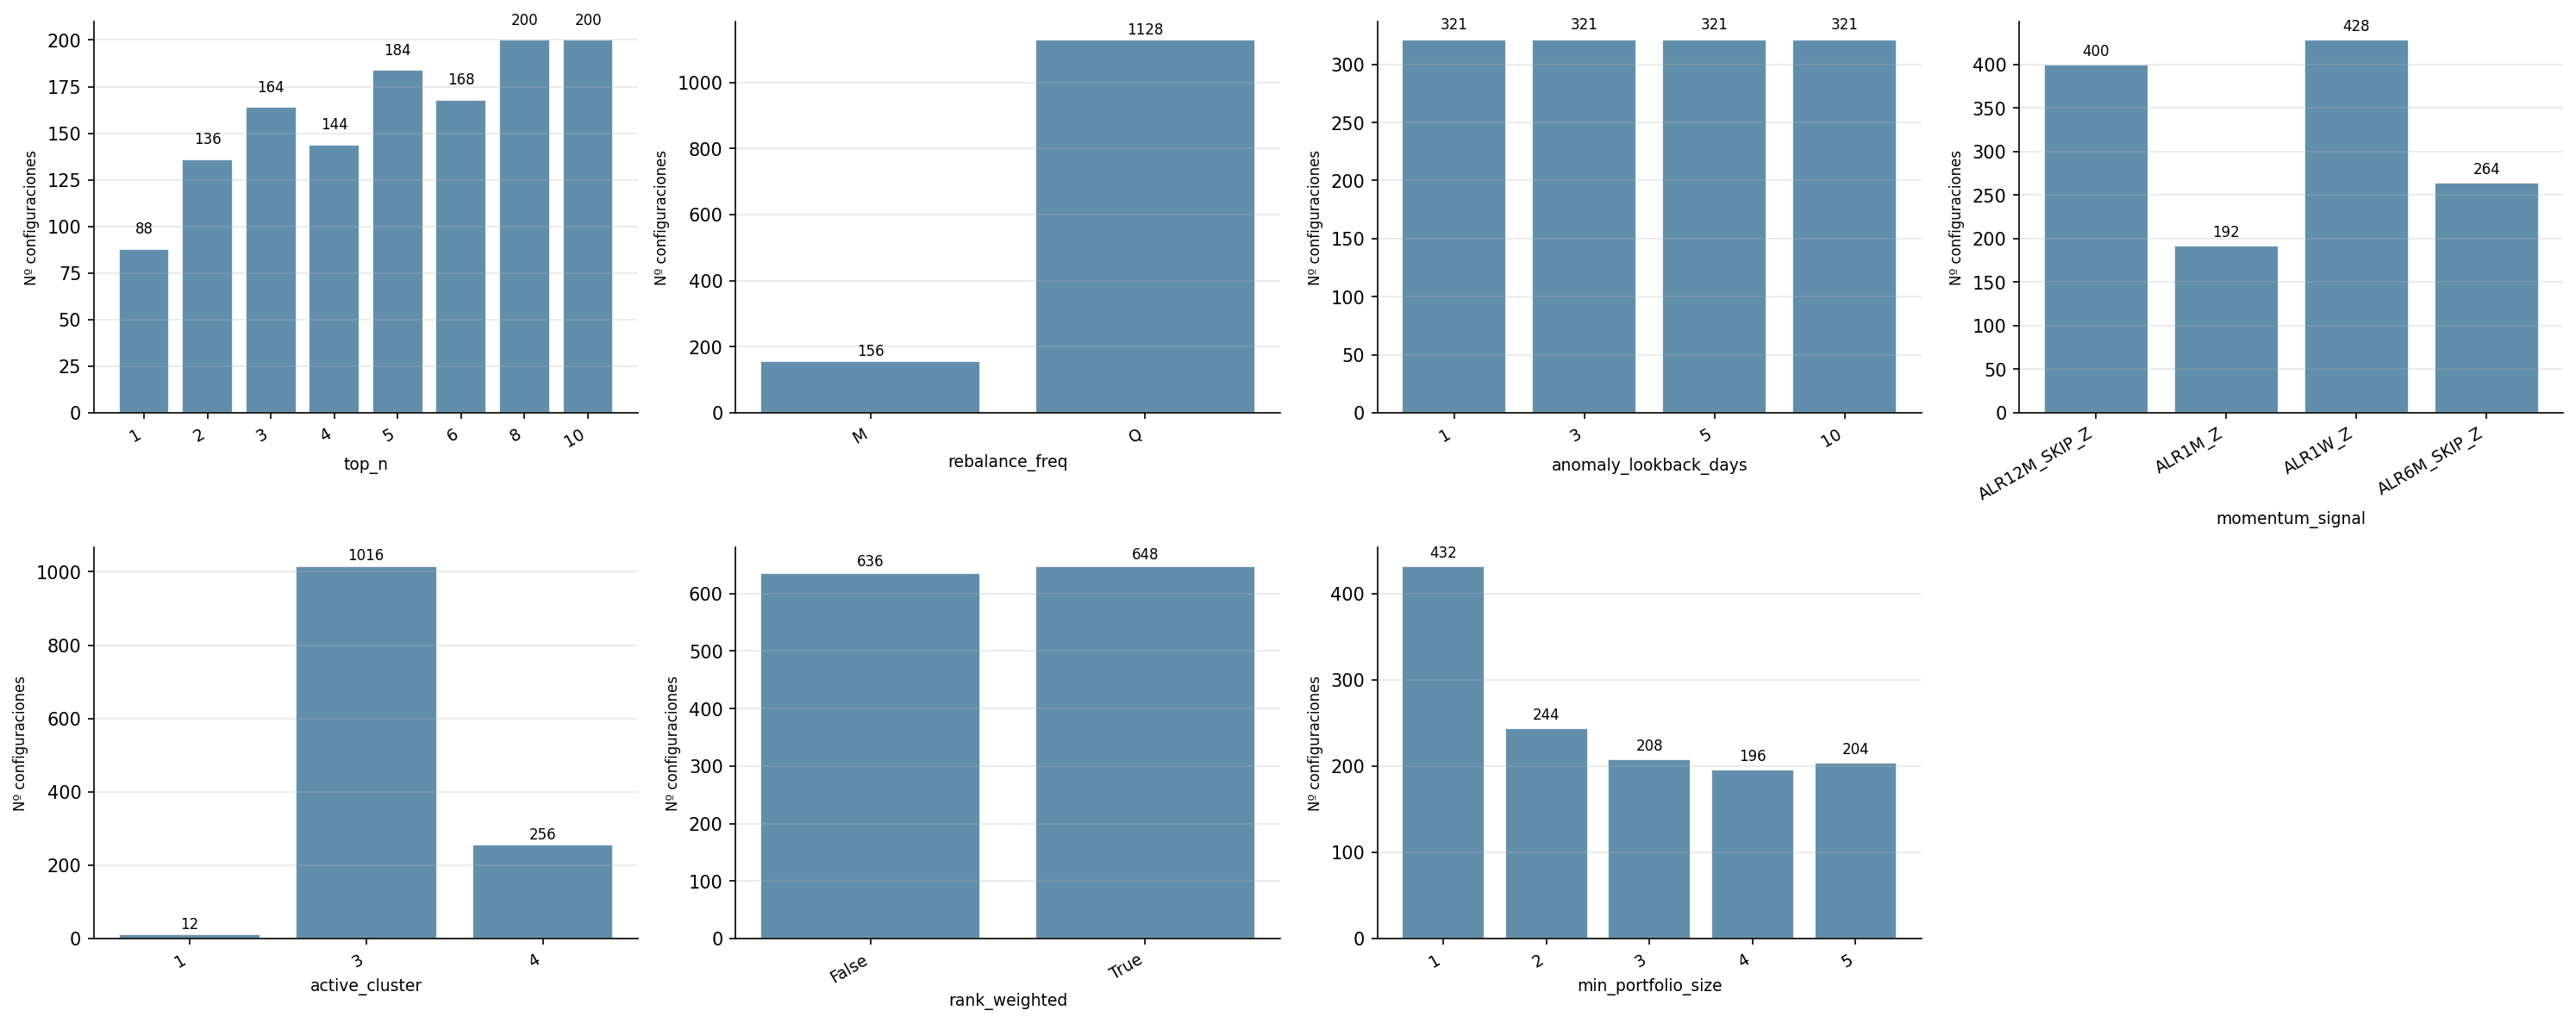
\includegraphics[width=\textwidth]{media/wf_04_hyperparameter_distribution.png}
    \caption{Distribución de hiperparámetros en el Top 10\,\%
    del Grid Search In-Sample. Cada barra representa el número de
    configuraciones (las mejores) que utilizan un valor concreto del
    parámetro. Fuente: Elaboración propia.}
    \label{fig:hyperparam_dist}
\end{figure}

Se observa que el parámetro \texttt{active\_cluster} presenta una
frecuencia enormemente concentrada en el valor 3 (Pullback
alcista), lo que indica que este régimen de mercado ofrece las
condiciones más favorables para la generación de señales de
momentum. Por el contrario, los clústeres 0 (Bajista moderado)
y 4 (Estrés/Capitulación) aparecen de forma marginal,
confirmando la interpretación económica desarrollada en el
Capítulo 4.

El rebalanceo trimestral (\texttt{Q}) domina ampliamente sobre el
mensual, los tamaños de cartera más frecuentes son
\texttt{top\_n=10} y \texttt{top\_n=8}, seguidos de
\texttt{top\_n=5} y \texttt{top\_n=3}, y la ponderación por ranking
(\texttt{rank\_weighted=True}) aparece con una frecuencia
ligeramente superior a la equiponderada, aunque ambas están
prácticamente equilibradas.

\paragraph{Top 5 combinaciones en entrenamiento}

La Tabla~\ref{tab:top5_is} presenta las cinco configuraciones con
mejor ratio de Sharpe dentro de la muestra de entrenamiento.

\begin{table}[H]
\centering
\small
\begin{tabular}{clcccccc}
\toprule
\textbf{\#} & \textbf{Señal} & \textbf{Cl.} & \textbf{Freq.} & \textbf{Top} &
\textbf{RW} & \textbf{Sharpe} & \textbf{CAGR (\%)} \\
\midrule
1 & ALR1W\_Z  & 3 & Q & 3 & No  & \textbf{1,366} & 26,63 \\
2 & ALR1W\_Z  & 3 & Q & 4 & Sí  & 1,298         & 26,78 \\
3 & ALR1W\_Z  & 3 & Q & 3 & No  & 1,293         & 24,84 \\
4 & ALR1W\_Z  & 3 & Q & 3 & Sí  & 1,285         & 26,91 \\
5 & ALR1W\_Z  & 3 & Q & 4 & No  & 1,281         & 25,34 \\
\bottomrule
\end{tabular}
\caption{Top 5 configuraciones del Grid Search In-Sample.
Fuente: Elaboración propia.}
\label{tab:top5_is}
\begin{flushleft}
\small \textit{Nota:} \textbf{Cl.}=active\_cluster,
\textbf{Freq.}=rebalance\_freq, \textbf{RW}=rank\_weighted.
\end{flushleft}
\end{table}

Se observa que la configuración óptima en entrenamiento alcanza
un ratio de Sharpe de 1,366 con una rentabilidad anualizada del
\SI{26,63}{\percent} y una caída máxima de únicamente \SI{-7.22}{\percent}. La
señal \texttt{ALR1W\_Z}, el clúster 3, el rebalanceo trimestral
y un tamaño de cartera reducido (\texttt{top\_n=3}) son los
elementos comunes a todas las configuraciones del Top 5.

No obstante, estas métricas deben interpretarse con cautela, ya
que reflejan el rendimiento sobre los mismos datos utilizados
para seleccionar la configuración. Habría que comprobar, tal y como se hará posteriormente, si este
rendimiento se mantiene al aplicarse sobre datos no vistos.


\subsubsection{Validación en Test}

Para evaluar la capacidad de generalización del sistema, las
1.280 configuraciones del Top 10\,\% en Sharpe de entrenamiento
se re-evaluaron sobre la ventana de prueba, que comprende el
último año de datos de mercado. 

\paragraph{Degradación del rendimiento}

La Tabla~\ref{tab:degradacion} muestra el comportamiento del conjunto de configuraciones al pasar de la ventana
de entrenamiento a la ventana de prueba.

\begin{table}[H]
\centering
\begin{tabular}{lrr}
\toprule
\textbf{Métrica} & \textbf{Train} & \textbf{Test} \\
\midrule
Sharpe medio                & 0,996   & 0,176    \\
CAGR medio (\%)             & 21,47   & 4,12     \\
Caída máxima media (\%)     & -17,82  & -18,24   \\
Proporción Sharpe $>$ 0 (\%)& 100,0   & 55,9     \\
Degradación de Sharpe media & ---     & 0,821    \\
\bottomrule
\end{tabular}
\caption{Métricas del proceso de validación sobre
1.280 configuraciones. Fuente: Elaboración propia.}
\label{tab:degradacion}
\end{table}

El descenso del Sharpe medio desde 0,996 hasta 0,176, con una
degradación media de 0,821 puntos, muestra la presencia de
sobreajuste (\textit{overfitting}) en el proceso
de selección. Esto es esperable y constituye una
característica común a cualquier proceso de optimización de
hiperparámetros sobre datos históricos.

Sin embargo, es relevante destacar que más de la mitad de las
configuraciones (55,9\,\%) mantienen un ratio de Sharpe positivo
en la ventana de prueba, lo que indica que existe un subconjunto de
estrategias con capacidad real de generalización.

\paragraph{La paradoja del campeón aparente}

La Figura~\ref{fig:sharpe_scatter} presenta un diagrama de
dispersión que muestra el Sharpe en entrenamiento (eje X)
frente al Sharpe en prueba (eje Y) para cada una de las 1.280
configuraciones evaluadas. Los puntos situados sobre la diagonal
representan estrategias que son consistentes; los que se
sitúan por debajo muestran degradación.

\begin{figure}[H]
    \centering
    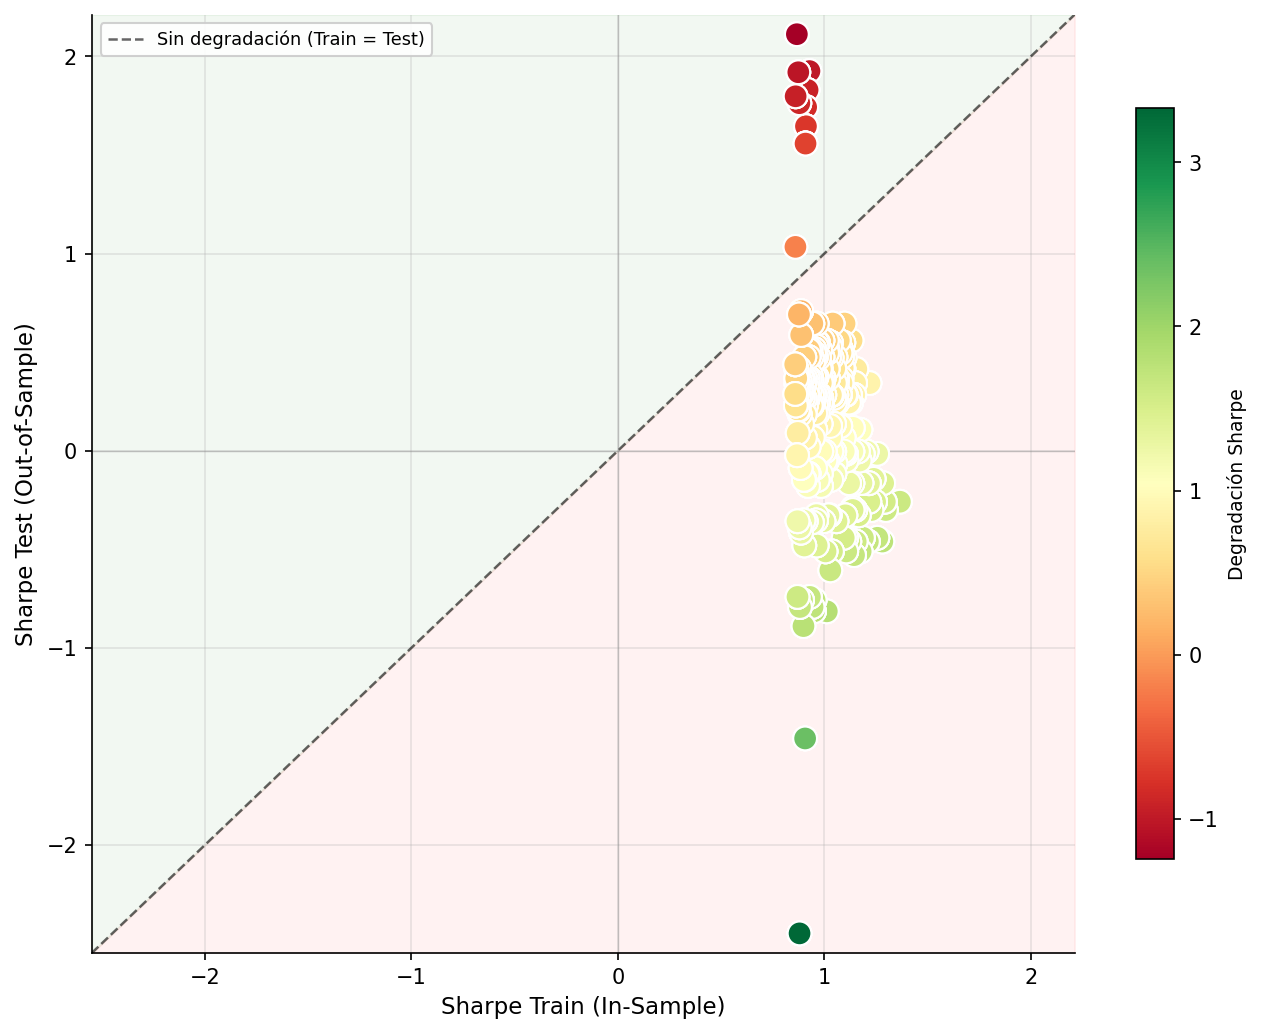
\includegraphics[width=0.8\textwidth]{media/wf_03_sharpe_scatter.png}
    \caption{Dispersión Sharpe Train vs.\ Sharpe Test. Cada punto
    representa una configuración. El color codifica la magnitud
    de la degradación (verde: baja, rojo: alta).
    Fuente: Elaboración propia.}
    \label{fig:sharpe_scatter}
\end{figure}

Se observa un fenómeno relevante: la configuración
con mejor Sharpe en entrenamiento (1,366) se sitúa en la zona
inferior del gráfico, con un Sharpe en prueba de \(-0,259\). Es
decir, la mejor estrategia aparente es, precisamente, la que más
fracasa al enfrentarse a datos nuevos. Este resultado constituye
una demostración de sobreajuste y muestra la
necesidad de la validación con datos no vistos.

Por el contrario, las configuraciones que mejores resultados
obtienen en Test no son las que lideraban el ranking en
entrenamiento. Esto refleja la existencia de
estrategias que, sin alcanzar los valores extremos de Sharpe en
la muestra de entrenamiento, poseen una estructura menos
sensible al ruido del periodo histórico.

\paragraph{Análisis de la degradación por ranking}

La Figura~\ref{fig:degradation_bar} muestra las barras
comparativas del ratio de Sharpe en entrenamiento y en prueba
para las configuraciones extremas del ranking. Se han
seleccionado las 15 configuraciones con menor Sharpe de
entrenamiento y las 15 con mayor Sharpe de entrenamiento.

\begin{figure}[H]
    \centering
    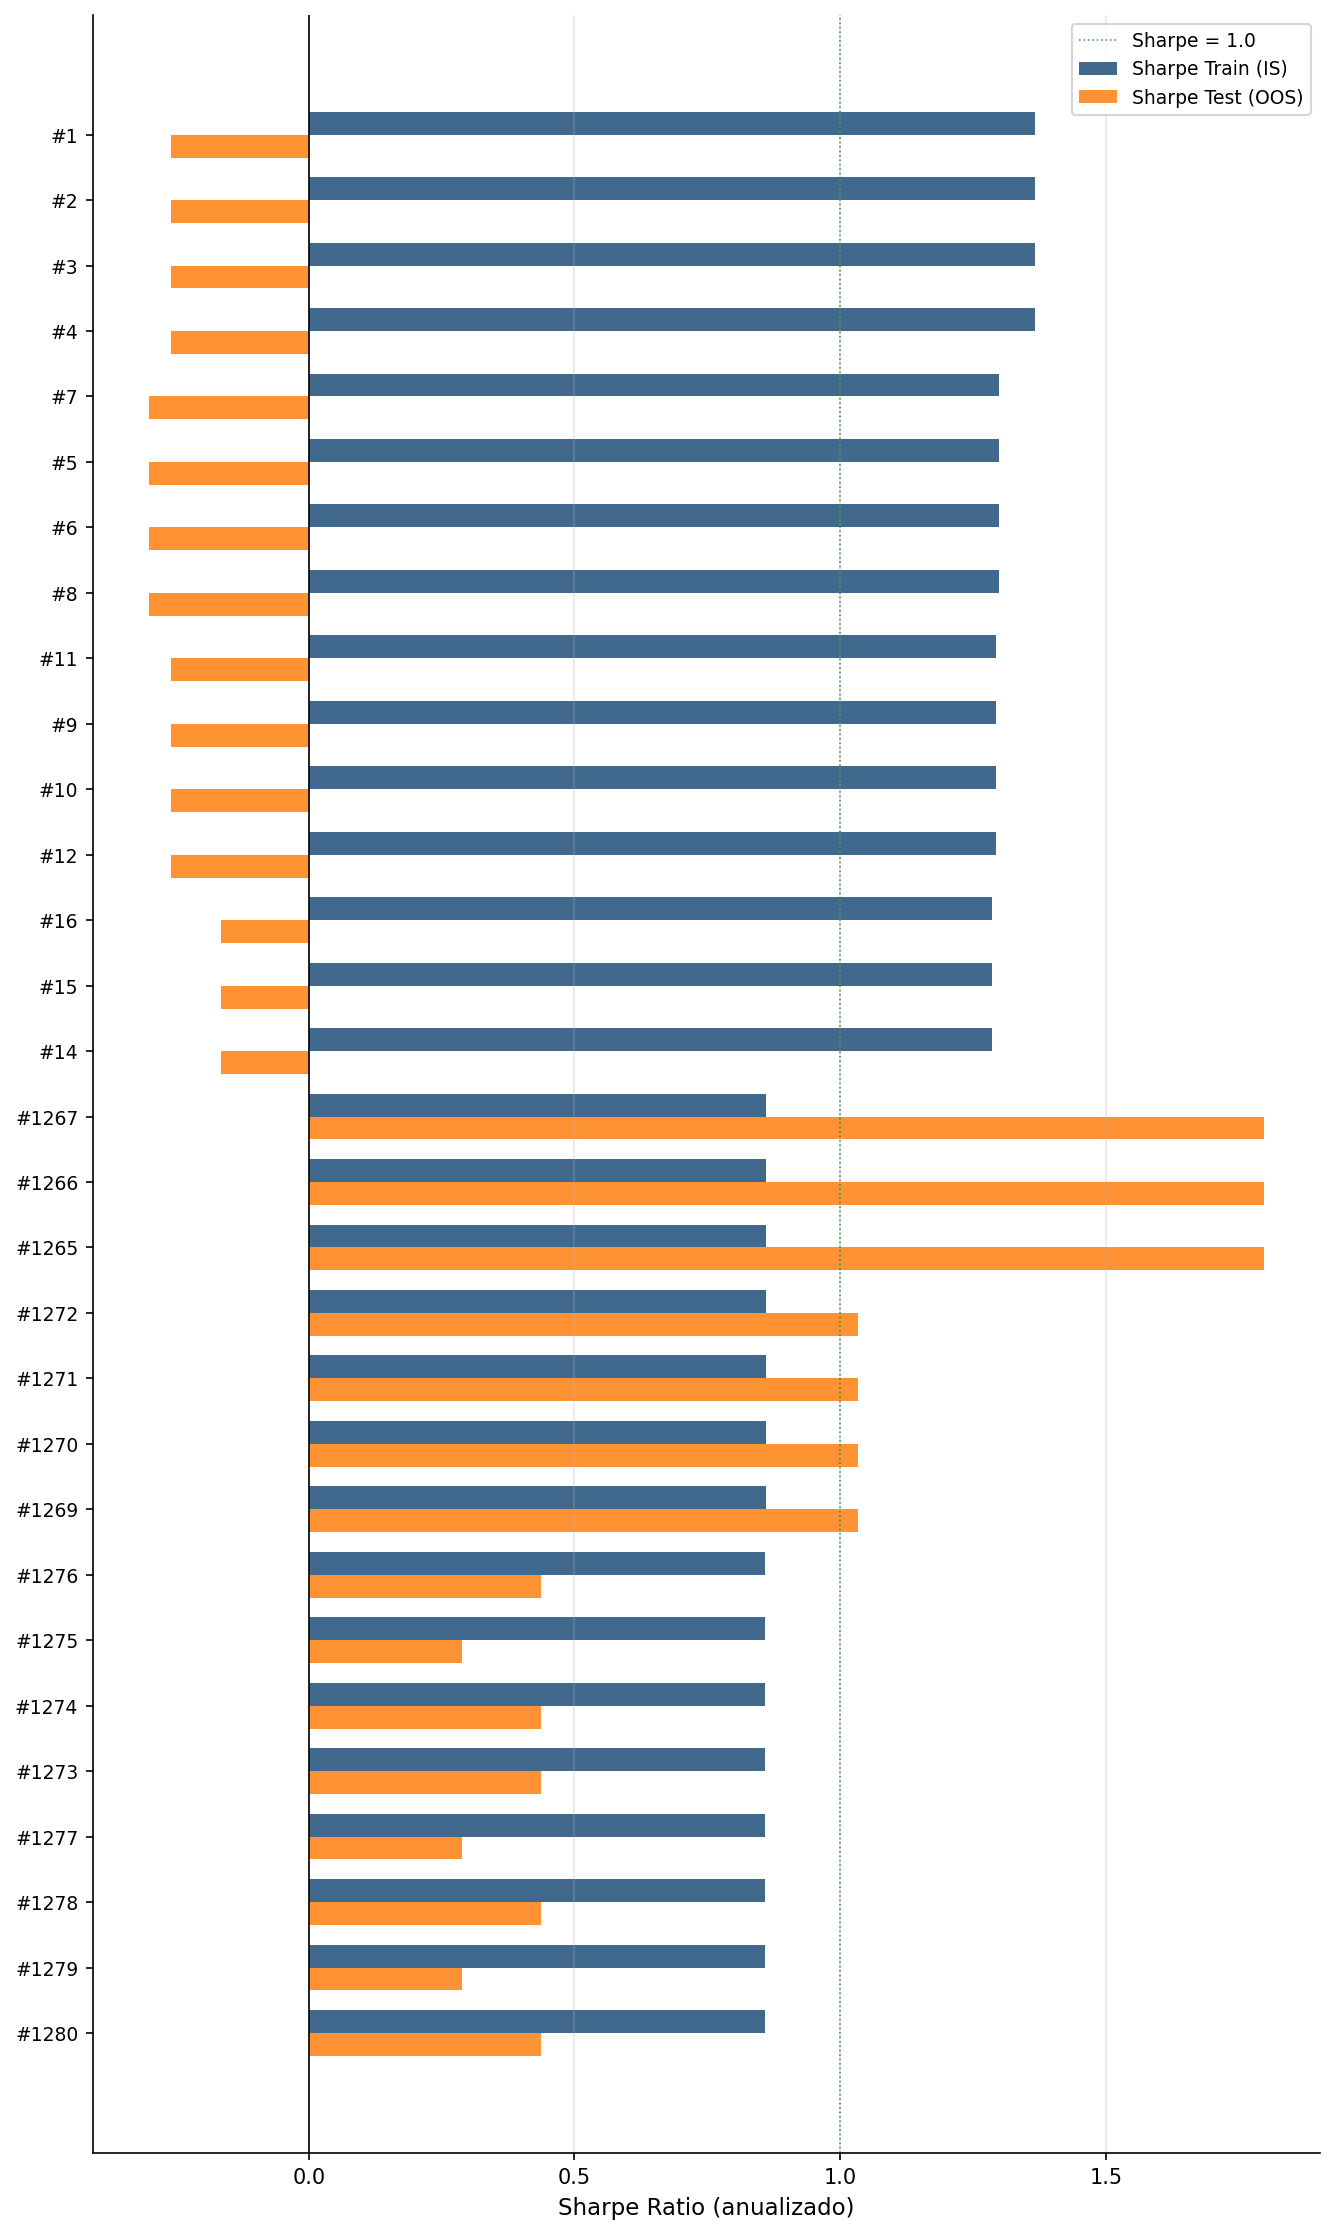
\includegraphics[width=0.85\textwidth]{media/wf_05_degradation_bar.png}
    \caption{Comparación del Sharpe en Train (azul) y en
    Test (naranja) para las configuraciones extremas. Se observa
    que las configuraciones con mayor Sharpe en entrenamiento
    presentan una degradación más elevada. Fuente: Elaboración propia.}
    \label{fig:degradation_bar}
\end{figure}

Se observa que las configuraciones con Sharpe de
entrenamiento más elevados muestran una caída
mayor en la ventana de Test. Este comportamiento refuerza la
necesidad de no confiar exclusivamente en las métricas de
entrenamiento para la selección del modelo final.

Por el contrario, las configuraciones con Sharpe de entrenamiento
moderado (en torno a 0,8--1,0) presentan, en muchos casos, una
degradación menor o incluso nula, lo que sugiere que estas
estrategias poseen una estructura más robusta.

\paragraph{Identificación de la mejor configuración global}

Se identifican las
configuraciones con mejor rendimiento en la ventana de prueba.
La Tabla~\ref{tab:top10_oos} presenta las diez estrategias con
Sharpe más elevado en datos no vistos.

\begin{table}[H]
\centering
\small
\begin{tabular}{clccccrr}
\toprule
\textbf{\#} & \textbf{Señal} & \textbf{Cl.} & \textbf{Freq.} & \textbf{Top} &
\textbf{RW} & \textbf{Sharpe\_Test} & \textbf{CAGR (\%)} \\
\midrule
1  & ALR1M\_Z    & 1 & M  & 8  & No  & \textbf{2,113} & 28,47 \\
2  & ALR1W\_Z    & 4 & M  & 3  & Sí  & 1,926         & 13,63 \\
3  & ALR1W\_Z    & 1 & M  & 10 & No  & 1,920         & 22,14 \\
4  & ALR1W\_Z    & 4 & M  & 4  & Sí  & 1,830         & 16,74 \\
5  & ALR1W\_Z    & 4 & M  & 5  & Sí  & 1,798         & 17,95 \\
6  & ALR1W\_Z    & 1 & M  & 10 & Sí  & 1,763         & 22,13 \\
7  & ALR1W\_Z    & 4 & M  & 2  & Sí  & 1,743         & 6,32  \\
8  & ALR1W\_Z    & 3 & Q  & 1  & No  & 1,646         & 16,72 \\
9  & ALR1W\_Z    & 3 & Q  & 1  & Sí  & 1,646         & 16,72 \\
10 & ALR1W\_Z    & 4 & M  & 3  & No  & 1,559         & 19,01 \\
\bottomrule
\end{tabular}
\caption{Top 10 configuraciones por Sharpe en Test.
Fuente: Elaboración propia.}
\label{tab:top10_oos}
\begin{flushleft}
\small \textit{Nota:} \textbf{Cl.}=active\_cluster,
\textbf{Freq.}=rebalance\_freq, \textbf{RW}=rank\_weighted.
\end{flushleft}
\end{table}

La mejor configuración global alcanza un ratio de Sharpe en
Test de 2,113, correspondiente a la señal \texttt{ALR1M\_Z}
(momento a un mes) sobre el clúster 1 (Bear market rally) con
rebalanceo mensual y tamaño de cartera \texttt{top\_n=8}. No
obstante, debe señalarse que este valor excepcional puede estar
influido por las condiciones específicas del periodo de prueba.

Las nueve configuraciones restantes del Top 10 comparten la
señal \texttt{ALR1W\_Z} (momento a una semana), lo que indica
que las señales de corto plazo son las que mejor se adaptan a
las condiciones del periodo de prueba. Destaca la diversidad
de regímenes representados: el clúster 4 (Estrés/Capitulación)
aparece en cinco configuraciones, el clúster 1 (Bear market
rally) en tres y el clúster 3 (Pullback alcista) en dos. El
rebalanceo mensual es mayoritario (ocho de diez), mientras que
la ponderación por ranking y la equiponderada se reparten al
50\,\%.

La configuración que ofrece el mejor equilibrio entre Sharpe
y rentabilidad dentro del grupo \texttt{ALR1W\_Z} es la que
combina el clúster 1 con \texttt{top\_n=10} y ponderación
equiponderada, alcanzando un Sharpe en Test de 1,920 y una
CAGR del 22,14\,\%.

\paragraph{Curva de capital de la configuración ganadora}

La Figura~\ref{fig:equity_winner} muestra la evolución del
capital acumulado de la mejor configuración en Test,
expresada en términos de mark-to-market diario real, frente al
índice de referencia SPY. La línea vertical punteada marca la
separación entre la ventana de entrenamiento y la ventana de
prueba.

\begin{figure}[H]
    \centering
    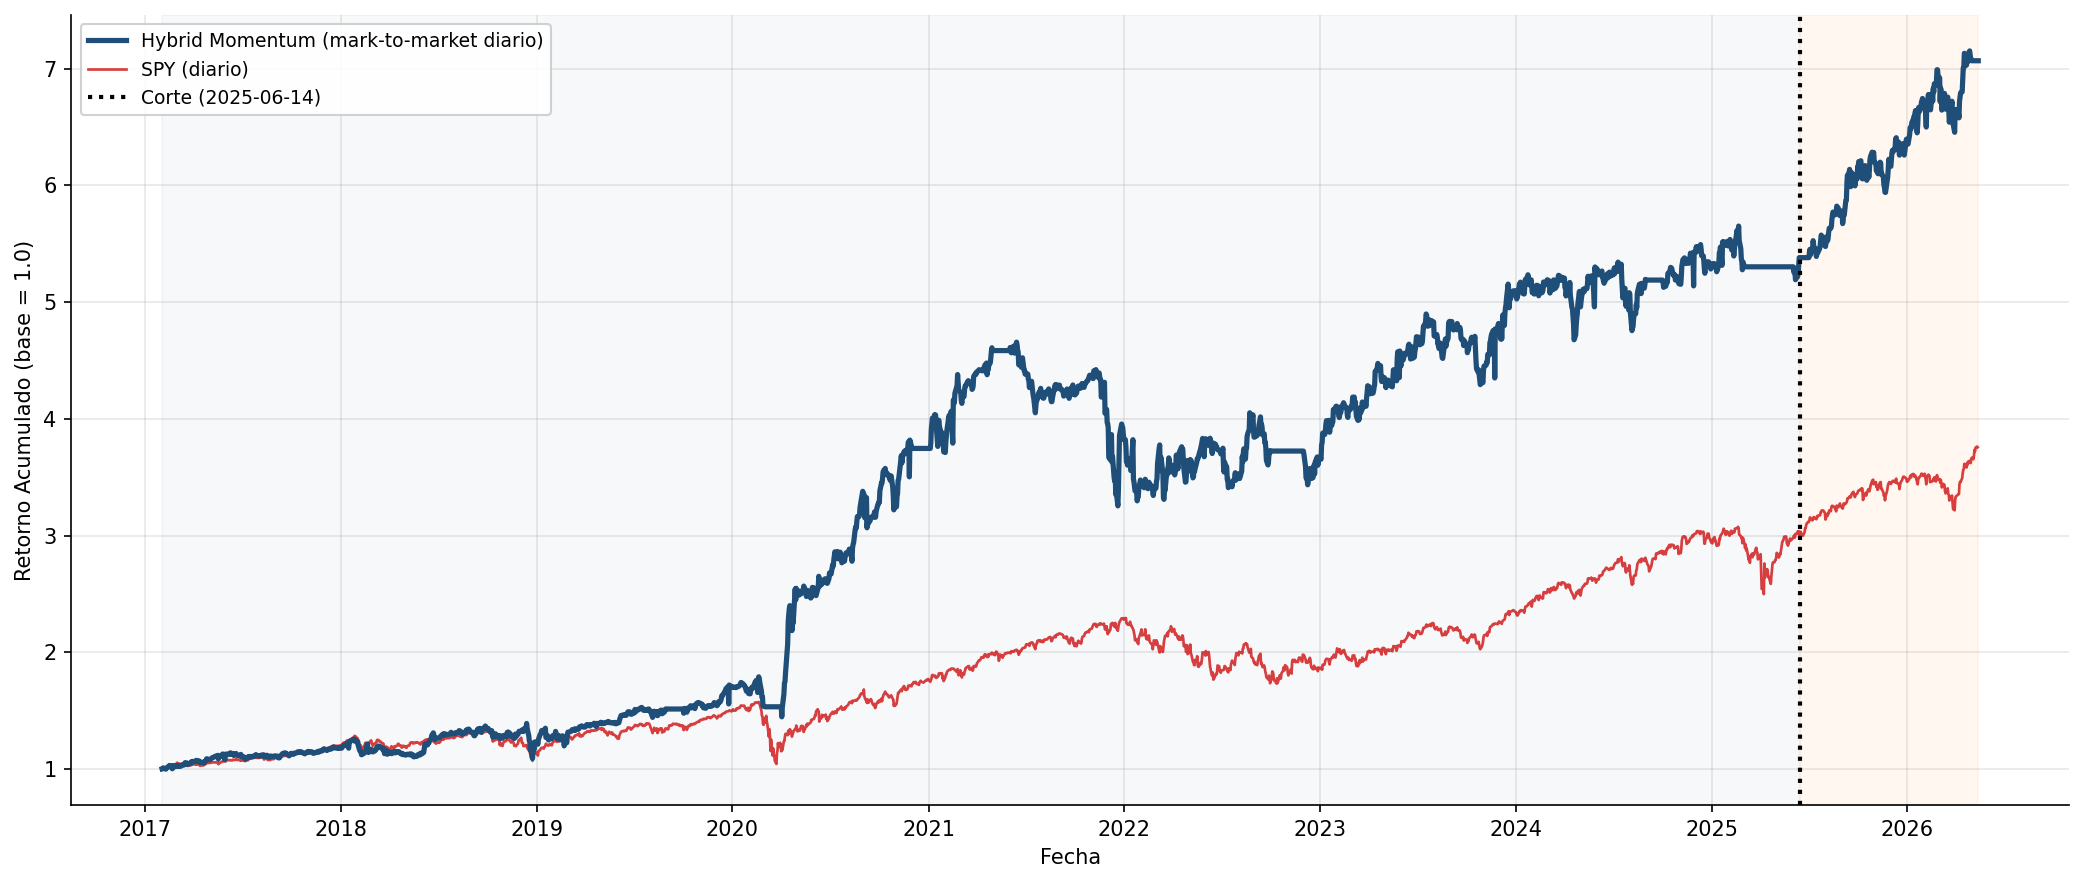
\includegraphics[width=\textwidth]{media/wf_01_equity_curve_winner_daily.png}
    \caption{Curva de capital de la mejor configuración
    en Test con resolución diaria frente al benchmark SPY.
    La línea vertical indica el inicio de la ventana de prueba.
    Fuente: Elaboración propia.}
    \label{fig:equity_winner}
\end{figure}

Se aprecia que la estrategia mantiene una trayectoria
ascendente consistente durante todo el periodo analizado,
acumulando una rentabilidad superior a la del
índice de referencia. La pendiente sostenida de la curva,
especialmente durante la ventana de prueba, sugiere que el
sistema es capaz de extraer señales de valor añadido de forma
consistente.

\paragraph{Comparativa con el índice de referencia SPY}

La Tabla~\ref{tab:comparativa_spy} presenta una comparación
entre las métricas de la mejor configuración
en Test y las del índice de referencia SPY.

\begin{table}[H]
\centering
\begin{tabular}{lrrr}
\toprule
\textbf{Métrica} & \textbf{Estrategia} & \textbf{SPY} \\
\midrule
Sharpe                & 2,113 & 0,585 \\
CAGR (\%)             & 28,47 & 12,10 \\
Caída máxima (\%)     & -4,05 & -12,10 \\
\bottomrule
\end{tabular}
\caption{Comparativa de la mejor configuración en Test frente al
benchmark SPY. Fuente: Elaboración propia.}
\label{tab:comparativa_spy}
\end{table}

La estrategia triplica prácticamente el ratio de Sharpe
del índice de referencia (2,113 frente a 0,585) y más que duplica
la rentabilidad anualizada (28,47\,\% frente a 12,10\,\%),
con una caída máxima notablemente inferior (-4,05\,\% frente a
-12,10\,\%). El sistema propuesto es capaz de generar
\textit{alpha} sobre el mercado de referencia.


\paragraph{Selección del modelo final}

Del análisis anterior se identifica como configuración de
referencia la estrategia \textbf{ALR1M\_Z} sobre el clúster 1
(Bear market rally), con rebalanceo mensual,
\texttt{top\_n=8} y ponderación equiponderada.

El criterio que justifica esta selección es:

\begin{itemize}
    \item \textbf{Rendimiento superior.} La estrategia triplica el
    Sharpe del índice de referencia (2,113 frente a 0,585) y más
    que duplica la rentabilidad anualizada (28,47\,\% frente a
    12,10\,\%), con una caída máxima de solo -4,05\,\% frente al
    -12,10\,\% del SPY.

    
\end{itemize}

No obstante, debe señalarse que este resultado excepcional
podría estar influido por las condiciones específicas del
periodo de prueba. Como alternativa más conservadora, las
configuraciones basadas en \texttt{ALR1W\_Z} ofrecen un
respaldo estadístico más amplio al concentrar nueve de las
diez posiciones del Top 10.

Los parámetros completos se resumen en la
Tabla~\ref{tab:modelo_final}.

\begin{table}[H]
\centering
\small
\begin{tabular}{ll}
\toprule
\textbf{Parámetro} & \textbf{Valor} \\
\midrule
Señal de momentum    & ALR1M\_Z (1 mes) \\
Clúster              & 1 (Bear market rally) \\
Rebalanceo           & Mensual (M) \\
Tamaño de cartera    & \texttt{top\_n=8} (8 activos) \\
Ponderación          & Equiponderada \\
Ventana anomalías    & 1 día \\
Tamaño mínimo cartera& 1 (sin mínimo exigido) \\
\bottomrule
\end{tabular}
\caption{Parámetros del modelo final seleccionado.
Fuente: Elaboración propia.}
\label{tab:modelo_final}
\end{table}


\subsubsection{Análisis de Robustez}

Esta sección aborda la cuestión de si los resultados obtenidos
pueden considerarse estadísticamente fiables o si, por el
contrario, responden a patrones 'falsos' propios del periodo de
evaluación.

\paragraph{Importancia de los hiperparámetros}

Para determinar qué parámetros del sistema ejercen una influencia
determinante sobre el rendimiento fuera de muestra, se ha
entrenado un modelo de bosque aleatorio (\textit{Random Forest})
con 300 árboles para predecir el Sharpe en prueba a partir de los
hiperparámetros de cada configuración. La
Tabla~\ref{tab:feature_importance} presenta la importancia
relativa de cada variable en la predicción.

\begin{table}[H]
\centering
\begin{tabular}{lr}
\toprule
\textbf{Variable} & \textbf{Importancia (\%)} \\
\midrule
top\_n                   & 25,99 \\
min\_portfolio\_size     & 23,64 \\
active\_cluster          & 21,01 \\
momentum\_signal         & 20,12 \\
rebalance\_freq          & 6,02  \\
rank\_weighted           & 3,22  \\
anomaly\_lookback\_days  & 0,01  \\
\bottomrule
\end{tabular}
\caption{Importancia de los hiperparámetros en la predicción del
Sharpe en Test mediante Random Forest. Fuente: Elaboración propia.}
\label{tab:feature_importance}
\end{table}

Los resultados revelan que los tres parámetros con mayor impacto
son \texttt{top\_n} (tamaño de la cartera), \texttt{min\_portfolio\_size}
(tamaño mínimo para evitar periodos en efectivo) y
\texttt{active\_cluster} (régimen de mercado seleccionado), que
conjuntamente explican más del 70\,\% de la varianza del
rendimiento fuera de muestra. La señal de momentum contribuye
con un 20\,\% adicional.

Resulta especialmente relevante la contribución prácticamente
nula del parámetro \texttt{anomaly\_lookback\_days} (ventana de
retrospectiva para el filtro DBSCAN). Este hallazgo sugiere que
la presencia del filtro topológico es importante para la
integridad del sistema, pero la longitud de la ventana de
observación de anomalías no es un factor determinante del
rendimiento, probablemente porque el filtro diario \textit{cross-
sectional} de DBSCAN proporciona una protección suficientemente
robusta con independencia del horizonte retrospectivo concreto
utilizado.

\paragraph{Sensibilidad de parámetros en ventana de prueba}

La Figura~\ref{fig:oos_sensitivity} descompone el rendimiento en Test agregado de las 1.064 configuraciones con Sharpe
de prueba válido, agrupándolas por el valor de cada
hiperparámetro. Para cada parámetro, se reconstruye la curva de
capital diaria de todas las configuraciones que comparten ese
valor y se promedia, permitiendo aislar visualmente el efecto
marginal de cada variable sobre el rendimiento conjunto.

\begin{figure}[H]
    \centering
    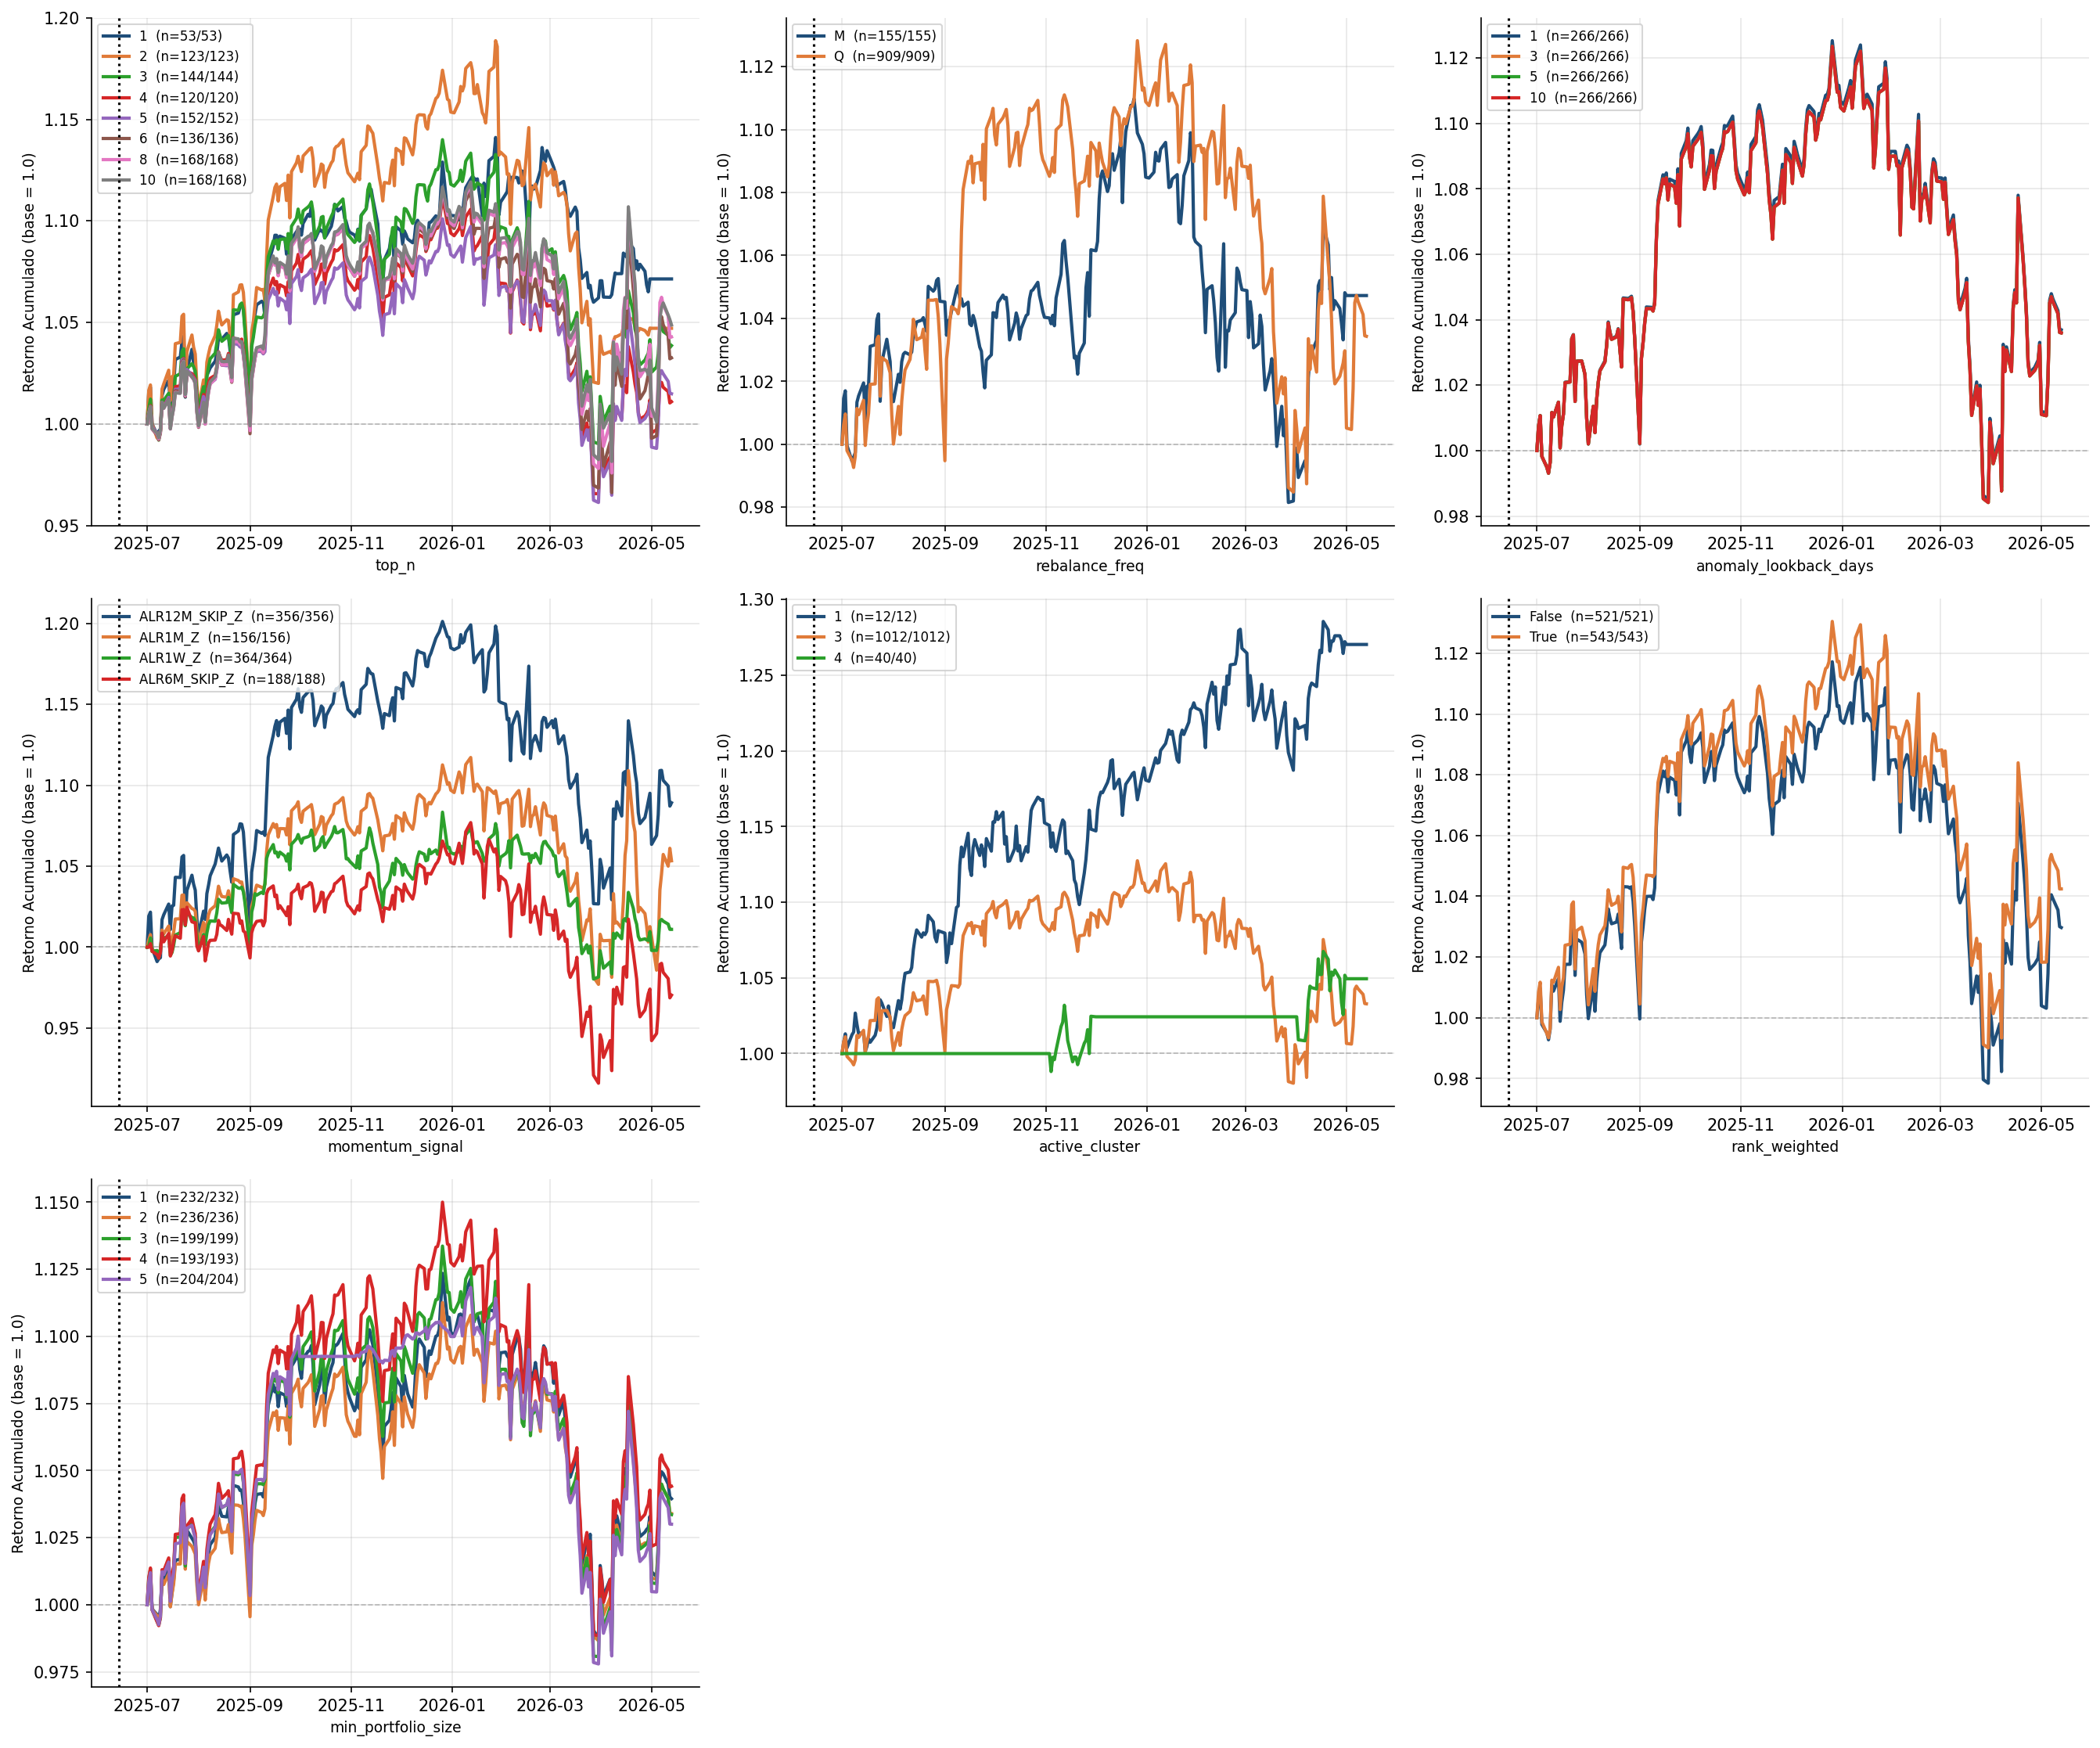
\includegraphics[width=1.05\textwidth]{media/wf_07_oos_parameter_sensitivity.png}
    \caption{Curvas de capital medias Out-of-Sample agrupadas por
    valor de hiperparámetro. Cada panel desagrega el efecto de
    una variable sobre el rendimiento agregado del conjunto de
    configuraciones (\textit{N}=1.064). Fuente: Elaboración propia.}
    \label{fig:oos_sensitivity}
\end{figure}

Se observa que:
\begin{itemize}
    
    \item \textbf{active\_cluster}: el clúster 1 es el que
    presenta el rendimiento acumulado medio más elevado (final
    de 1,270), seguido del clúster 4 (1,050). El clúster 3,
    pese a concentrar el 95\,\% de las configuraciones,
    muestra la curva media más baja (1,033).
    
    \item \textbf{rebalance\_freq}: la frecuencia mensual
    (\texttt{M}) supera a la trimestral en rendimiento acumulado
    medio (1,047 frente a 1,034), pese a que esta última
    concentra el 85\,\% de las configuraciones.
    \item \textbf{rank\_weighted}: la ponderación por ranking
    ofrece un rendimiento ligeramente superior a la
    equiponderada (1,042 frente a 1,030), aunque la diferencia
    es muy leve y ambas opciones generan rentabilidad positiva
    en promedio.
\end{itemize}

\paragraph{Conclusiones del capítulo}

Los resultados presentados a lo largo de este capítulo permiten
extraer las siguientes conclusiones consolidadas:

\begin{enumerate}
    \item \textbf{El sobreajuste existe y es significativo.} La
    mejor configuración en entrenamiento (Sharpe 1,366) presenta
    un rendimiento negativo en la ventana de prueba (\(-0,259\)).
    Este fenómeno es común a cualquier proceso de optimización
    sobre datos históricos y debe ser gestionado mediante
    validación con datos no vistos.

    \item \textbf{La robustez existe y es identificable.} El
    55,9\,\% de las configuraciones mantienen un Sharpe positivo
    en prueba, y la mejor de ellas alcanza un valor de 2,113
    (señal \texttt{ALR1M\_Z} sobre clúster 1, rebalanceo mensual,
    \texttt{top\_n=8}). Esta configuración se consolida como el
    modelo de referencia del sistema.

    \item \textbf{El sistema supera al benchmark de referencia.}
    Tanto en términos de Sharpe (2,113 frente a 0,585) como de
    CAGR (28,47\,\% frente a 12,10\,\%), la mejor configuración
    en Test triplica el rendimiento ajustado al riesgo del
    índice SPY, con una caída máxima notablemente inferior.

    \item \textbf{La selección del régimen de mercado es
    crítica.} El parámetro \texttt{active\_cluster} explica el
    21\,\% de la varianza del rendimiento fuera de muestra. El
    clúster 3 (Pullback alcista) se consolida como el régimen
    más favorable para estrategias basadas en momentum.

    \item \textbf{El filtro topológico DBSCAN es un componente
    estructural, no una variable de ajuste.} La ventana de
    retrospectiva para la detección de anomalías (\texttt{anomaly\_lookback\_days})
    presenta una importancia prácticamente nula en el modelo de
    predicción, lo que sugiere que la presencia del filtro DBSCAN proporciona una protección
    suficiente contra el ruido.
\end{enumerate}

A la vista de estos resultados, el modelo seleccionado como
configuración de referencia es la estrategia
\texttt{ALR1M\_Z} sobre el clúster 1, con rebalanceo
mensual, \texttt{top\_n=8} y ponderación equiponderada.
Esta configuración ofrece la mayor rentabilidad, superando
al índice de referencia SPY tanto en términos
de Sharpe como de rentabilidad anualizada.


\endinput

% =============================================================================

\subsection{Evaluación y Backtesting}

En este capítulo se describe la evaluación
diseñada para validar el modelo propuesto, se presentan
los resultados obtenidos tanto en la fase de
entrenamiento (Train) como en la fase de prueba
(Test) y se analiza la robustez de las
configuraciones analizadas. El objetivo fundamental es
determinar si la arquitectura DBSCAN + K-Means,
combinada con una selección dinámica por momentum, es capaz de
generar rentabilidades (teniendo en cuenta el riesgo) superiores a las de
un índice de referencia.

A lo largo del capítulo se analiza si existe una combinación de hiperparámetros que responda de forma estable a datos no vistos, se cuantifica la magnitud de la degradación por sobreajuste al seleccionar las mejores configuraciones en la muestra de entrenamiento, y se identifican los parámetros que tienen una influencia sobre el rendimiento en test.


\subsubsection{Sistema de Evaluación}

La validación del sistema se ha diseñado con el objetivo de
aproximar, en la medida de lo posible, un entorno real de
inversión. Para ello, se establecen una serie de criterios orientados a evitar sesgos y a garantizar que la
comparación entre estrategias sea homogénea.

\paragraph{Causalidad temporal ($T/T+1$)}

Las decisiones de inversión se generan únicamente con la
información disponible al cierre del último día hábil del período
de rebalanceo $T$. La entrada efectiva en cartera se realiza al
cierre del primer día hábil posterior ($T+1$). De esta forma,
se evita incorporar información futura en el proceso de decisión.

Los retornos de cada cartera se calculan desde el cierre de
$T+1$ hasta el cierre del siguiente período de rebalanceo.
Además, todas las transformaciones estadísticas utilizadas por
el modelo se estiman
exclusivamente con datos históricos disponibles en cada fecha
según la Ecuación~\ref{eq:zscore_rolling}.

\paragraph{Ventanas temporales y división Train/Test}

El periodo completo de análisis comprende desde enero de 2017
hasta la fecha más reciente disponible. Para garantizar la
independencia entre la fase de optimización y la fase de
validación, se establece un punto de corte dinámico situado
exactamente un año antes del momento de ejecución del
experimento:

\begin{itemize}
    \item \textbf{Ventana de entrenamiento (Train):}
    desde enero de 2017 hasta un año antes de la fecha actual.
    Sobre esta ventana se ejecuta el \textit{grid search}.
    \item \textbf{Ventana de prueba (Test):}
    desde la fecha de corte hasta la actualidad. Sobre esta
    ventana se evalúan exclusivamente las configuraciones
    seleccionadas en la fase de entrenamiento, sin ningún tipo
    de realimentación hacia el modelo.
\end{itemize}

\paragraph{Benchmark de referencia}

Como índice de comparación se utiliza el ETF \textit{SPDR
S\&P 500 ETF Trust} (SPY), ampliamente empleado como referencia de la renta variable estadounidense. Su curva de
capital se normaliza a base 1,0 en la misma fecha inicial que la
estrategia.

\paragraph{Arquitectura del proceso experimental}

El diseño sigue dos etapas diferenciadas, ilustrado en la
Figura~\ref{fig:experimental_design}:

\begin{enumerate}
    \item \textbf{Búsqueda en malla (\textit{Grid Search})
    con datos de entrenamiento}: Se enumeran las 12.800
    combinaciones resultantes de los
    siete hiperparámetros definidos en el sistema
    (\texttt{top\_n}, \texttt{rebalance\_freq},
    \texttt{anomaly\_lookback\_days}, \texttt{momentum\_signal},
    \texttt{active\_cluster}, \texttt{rank\_weighted} y
    \texttt{min\_portfolio\_size}). Cada combinación se evalúa
    sobre la ventana de entrenamiento y se registran sus
    métricas.

    \item \textbf{Validación con datos de prueba}: Se
    selecciona el 10\,\% de las configuraciones con mejor
    \textit{ratio de Sharpe} en la fase anterior (1.280 estrategias). Cada una de ellas se re-evalúa sobre la
    ventana de Test, cronológicamente posterior y nunca vista
    durante la optimización. Se mide la degradación del Sharpe
    como diferencia entre el valor en entrenamiento y en prueba,
    siendo la métrica central de sobreajuste.
\end{enumerate}

\begin{figure}[H]
    \centering
    \begin{tikzpicture}[node distance=1.5cm, auto,
        block/.style={rectangle, draw, text width=7cm,
        text centered, rounded corners, minimum height=0.8cm,
        font=\small},
        arrow/.style={draw, -latex', thick}]

        \node [block, fill=green!10] (grid)
            {Grid Search \\
             7 parámetros $\times$ 12.800 combinaciones \\
             Ventana: 2017 -- ($t-1$ año)};
        \node [block, below of=grid, fill=yellow!15] (top)
            {Selección Top 10\,\% por Sharpe \\
             $\approx$ 1.280 configuraciones \\};
        \node [block, below of=top, fill=cyan!15] (wf)
            {Evaluación en datos de prueba \\
             Ventana: ($t-1$ año) -- ($t$) \\
             Sharpe\_Test, Degradación};
        \node [block, below of=wf, fill=orange!15] (analysis)
            {Análisis de Robustez \\
             Importancia de parámetros, \\
             Sensibilidad, Comparativa vs SPY};

        \path [arrow] (grid) -- (top);
        \path [arrow] (top) -- (wf);
        \path [arrow] (wf) -- (analysis);
    \end{tikzpicture}
    \caption{Arquitectura del proceso experimental. Fuente: Elaboración propia.}
    \label{fig:experimental_design}
\end{figure}


\subsubsection{Búsqueda en malla (Grid Search) en datos de entrenamiento}

Sobre la ventana de entrenamiento se ejecuta un barrido de las 12.800 combinaciones de hiperparámetros
ya mencionadas. Todas las combinaciones
generaron resultados válidos.

\paragraph{Distribución del ratio de Sharpe en entrenamiento}

La Figura~\ref{fig:hyperparam_dist} muestra la distribución de
los siete hiperparámetros dentro del subconjunto de estrategias
que pertenecen al 10\,\% superior en Sharpe dentro de la muestra
de entrenamiento. Este análisis permite identificar qué valores
de cada parámetro aparecen con mayor frecuencia entre las mejores
configuraciones.

\begin{figure}[H]
    \centering
    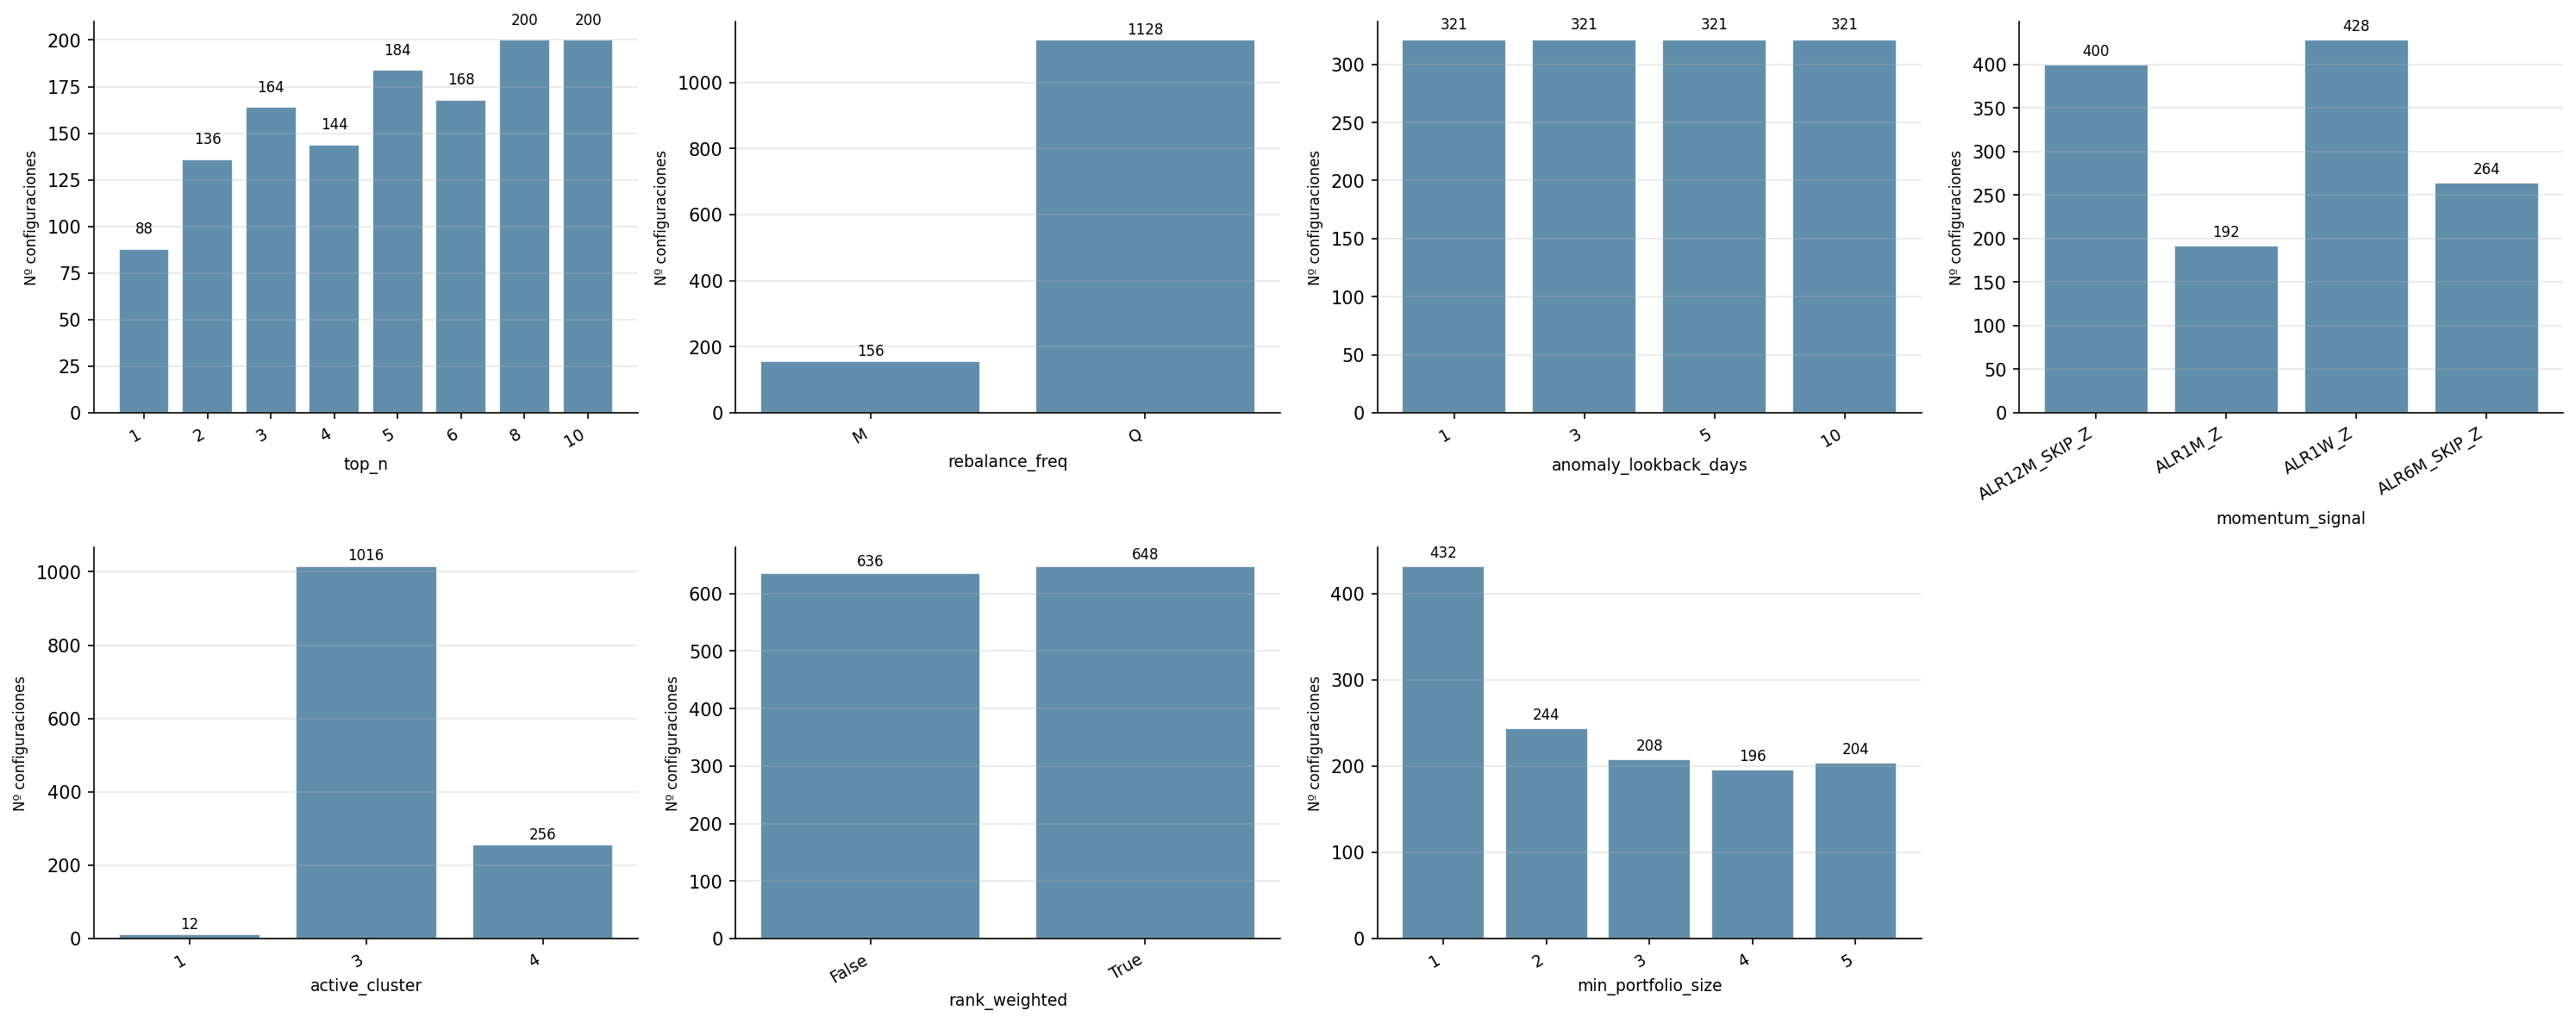
\includegraphics[width=\textwidth]{media/wf_04_hyperparameter_distribution.png}
    \caption{Distribución de hiperparámetros en el Top 10\,\%
    del Grid Search In-Sample. Cada barra representa el número de
    configuraciones (las mejores) que utilizan un valor concreto del
    parámetro. Fuente: Elaboración propia.}
    \label{fig:hyperparam_dist}
\end{figure}

Se observa que el parámetro \texttt{active\_cluster} presenta una
frecuencia enormemente concentrada en el valor 3 (Pullback
alcista), lo que indica que este régimen de mercado ofrece las
condiciones más favorables para la generación de señales de
momentum. Por el contrario, los clústeres 0 (Bajista moderado)
y 4 (Estrés/Capitulación) aparecen de forma marginal,
confirmando la interpretación económica desarrollada en el
Capítulo 4.

El rebalanceo trimestral (\texttt{Q}) domina ampliamente sobre el
mensual, los tamaños de cartera más frecuentes son
\texttt{top\_n=10} y \texttt{top\_n=8}, seguidos de
\texttt{top\_n=5} y \texttt{top\_n=3}, y la ponderación por ranking
(\texttt{rank\_weighted=True}) aparece con una frecuencia
ligeramente superior a la equiponderada, aunque ambas están
prácticamente equilibradas.

\paragraph{Top 5 combinaciones en entrenamiento}

La Tabla~\ref{tab:top5_is} presenta las cinco configuraciones con
mejor ratio de Sharpe dentro de la muestra de entrenamiento.

\begin{table}[H]
\centering
\small
\begin{tabular}{clcccccc}
\toprule
\textbf{\#} & \textbf{Señal} & \textbf{Cl.} & \textbf{Freq.} & \textbf{Top} &
\textbf{RW} & \textbf{Sharpe} & \textbf{CAGR (\%)} \\
\midrule
1 & ALR1W\_Z  & 3 & Q & 3 & No  & \textbf{1,366} & 26,63 \\
2 & ALR1W\_Z  & 3 & Q & 4 & Sí  & 1,298         & 26,78 \\
3 & ALR1W\_Z  & 3 & Q & 3 & No  & 1,293         & 24,84 \\
4 & ALR1W\_Z  & 3 & Q & 3 & Sí  & 1,285         & 26,91 \\
5 & ALR1W\_Z  & 3 & Q & 4 & No  & 1,281         & 25,34 \\
\bottomrule
\end{tabular}
\caption{Top 5 configuraciones del Grid Search In-Sample.
Fuente: Elaboración propia.}
\label{tab:top5_is}
\begin{flushleft}
\small \textit{Nota:} \textbf{Cl.}=active\_cluster,
\textbf{Freq.}=rebalance\_freq, \textbf{RW}=rank\_weighted.
\end{flushleft}
\end{table}

Se observa que la configuración óptima en entrenamiento alcanza
un ratio de Sharpe de 1,366 con una rentabilidad anualizada del
\SI{26,63}{\percent} y una caída máxima de únicamente \SI{-7.22}{\percent}. La
señal \texttt{ALR1W\_Z}, el clúster 3, el rebalanceo trimestral
y un tamaño de cartera reducido (\texttt{top\_n=3}) son los
elementos comunes a todas las configuraciones del Top 5.

No obstante, estas métricas deben interpretarse con cautela, ya
que reflejan el rendimiento sobre los mismos datos utilizados
para seleccionar la configuración. Habría que comprobar, tal y como se hará posteriormente, si este
rendimiento se mantiene al aplicarse sobre datos no vistos.


\subsubsection{Validación en Test}

Para evaluar la capacidad de generalización del sistema, las
1.280 configuraciones del Top 10\,\% en Sharpe de entrenamiento
se re-evaluaron sobre la ventana de prueba, que comprende el
último año de datos de mercado. 

\paragraph{Degradación del rendimiento}

La Tabla~\ref{tab:degradacion} muestra el comportamiento del conjunto de configuraciones al pasar de la ventana
de entrenamiento a la ventana de prueba.

\begin{table}[H]
\centering
\begin{tabular}{lrr}
\toprule
\textbf{Métrica} & \textbf{Train} & \textbf{Test} \\
\midrule
Sharpe medio                & 0,996   & 0,176    \\
CAGR medio (\%)             & 21,47   & 4,12     \\
Caída máxima media (\%)     & -17,82  & -18,24   \\
Proporción Sharpe $>$ 0 (\%)& 100,0   & 55,9     \\
Degradación de Sharpe media & ---     & 0,821    \\
\bottomrule
\end{tabular}
\caption{Métricas del proceso de validación sobre
1.280 configuraciones. Fuente: Elaboración propia.}
\label{tab:degradacion}
\end{table}

El descenso del Sharpe medio desde 0,996 hasta 0,176, con una
degradación media de 0,821 puntos, muestra la presencia de
sobreajuste (\textit{overfitting}) en el proceso
de selección. Esto es esperable y constituye una
característica común a cualquier proceso de optimización de
hiperparámetros sobre datos históricos.

Sin embargo, es relevante destacar que más de la mitad de las
configuraciones (55,9\,\%) mantienen un ratio de Sharpe positivo
en la ventana de prueba, lo que indica que existe un subconjunto de
estrategias con capacidad real de generalización.

\paragraph{La paradoja del campeón aparente}

La Figura~\ref{fig:sharpe_scatter} presenta un diagrama de
dispersión que muestra el Sharpe en entrenamiento (eje X)
frente al Sharpe en prueba (eje Y) para cada una de las 1.280
configuraciones evaluadas. Los puntos situados sobre la diagonal
representan estrategias que son consistentes; los que se
sitúan por debajo muestran degradación.

\begin{figure}[H]
    \centering
    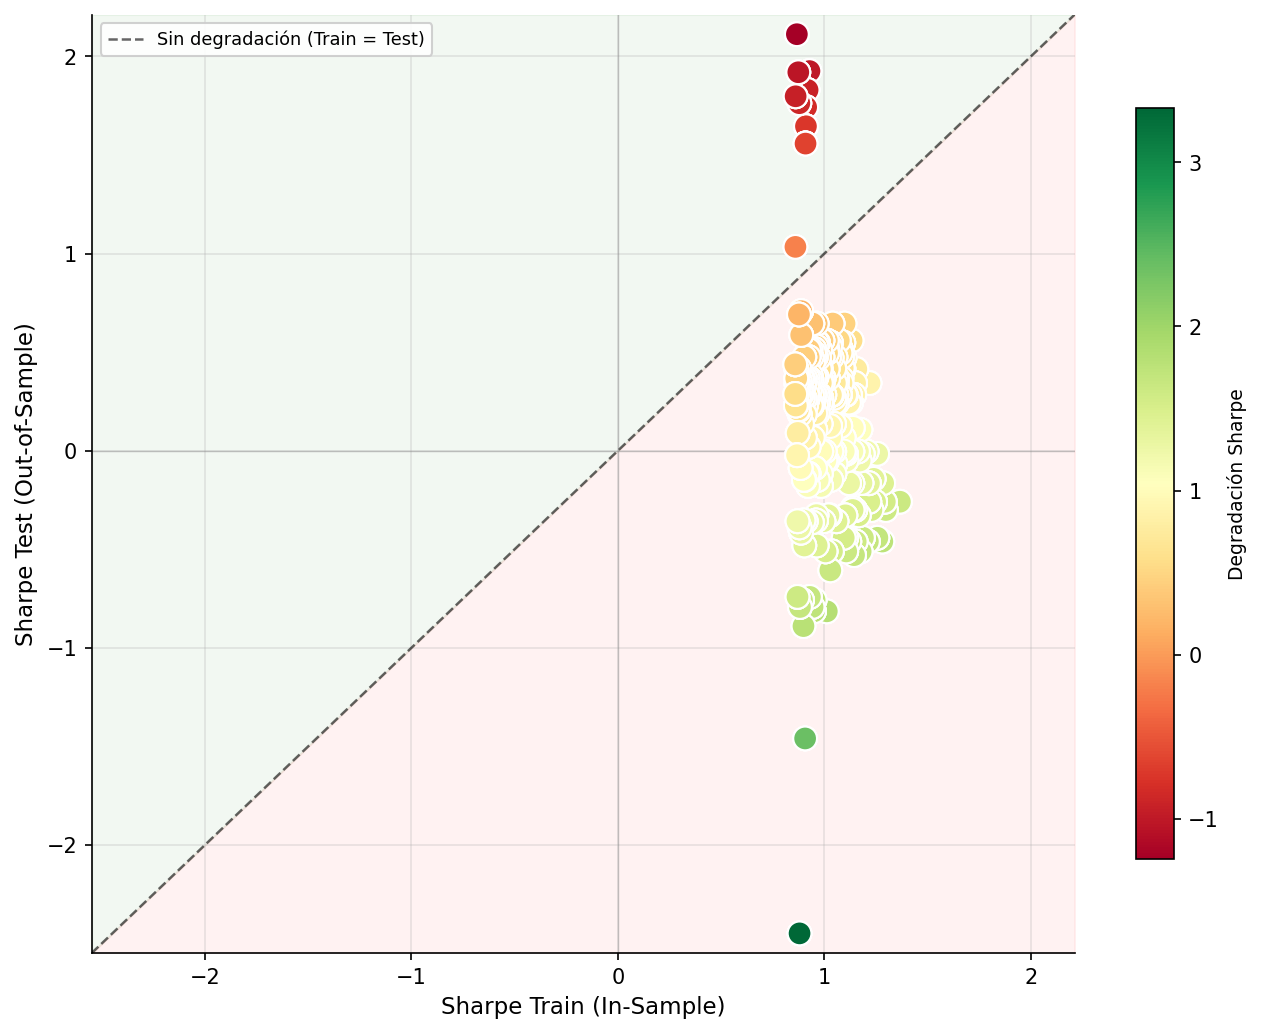
\includegraphics[width=0.8\textwidth]{media/wf_03_sharpe_scatter.png}
    \caption{Dispersión Sharpe Train vs.\ Sharpe Test. Cada punto
    representa una configuración. El color codifica la magnitud
    de la degradación (verde: baja, rojo: alta).
    Fuente: Elaboración propia.}
    \label{fig:sharpe_scatter}
\end{figure}

Se observa un fenómeno relevante: la configuración
con mejor Sharpe en entrenamiento (1,366) se sitúa en la zona
inferior del gráfico, con un Sharpe en prueba de \(-0,259\). Es
decir, la mejor estrategia aparente es, precisamente, la que más
fracasa al enfrentarse a datos nuevos. Este resultado constituye
una demostración de sobreajuste y muestra la
necesidad de la validación con datos no vistos.

Por el contrario, las configuraciones que mejores resultados
obtienen en Test no son las que lideraban el ranking en
entrenamiento. Esto refleja la existencia de
estrategias que, sin alcanzar los valores extremos de Sharpe en
la muestra de entrenamiento, poseen una estructura menos
sensible al ruido del periodo histórico.

\paragraph{Análisis de la degradación por ranking}

La Figura~\ref{fig:degradation_bar} muestra las barras
comparativas del ratio de Sharpe en entrenamiento y en prueba
para las configuraciones extremas del ranking. Se han
seleccionado las 15 configuraciones con menor Sharpe de
entrenamiento y las 15 con mayor Sharpe de entrenamiento.

\begin{figure}[H]
    \centering
    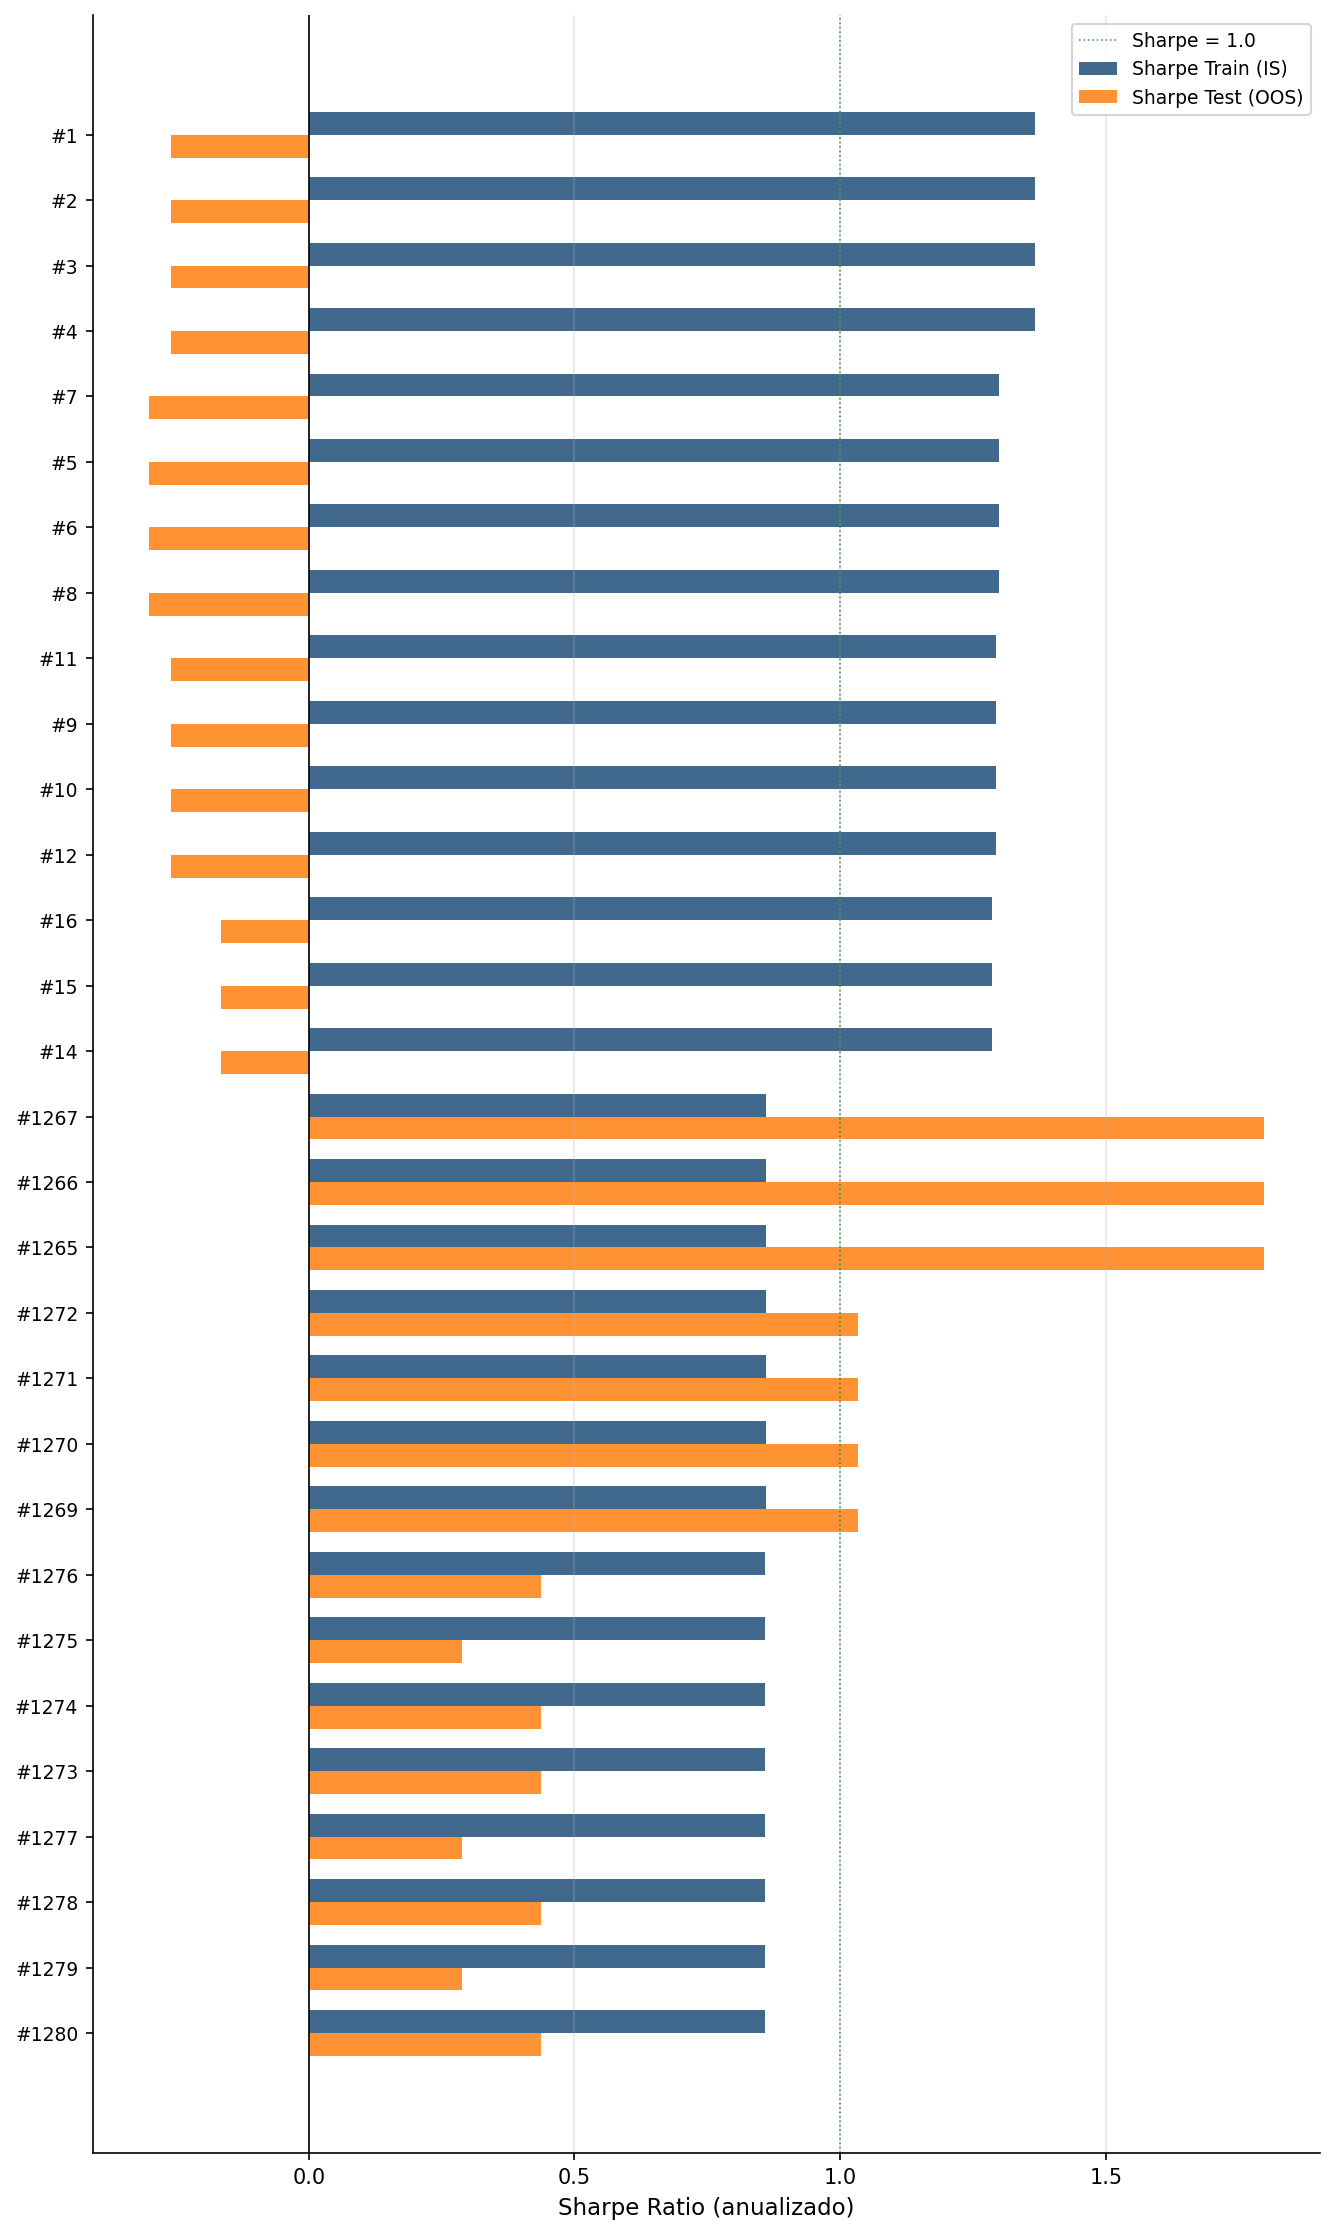
\includegraphics[width=0.85\textwidth]{media/wf_05_degradation_bar.png}
    \caption{Comparación del Sharpe en Train (azul) y en
    Test (naranja) para las configuraciones extremas. Se observa
    que las configuraciones con mayor Sharpe en entrenamiento
    presentan una degradación más elevada. Fuente: Elaboración propia.}
    \label{fig:degradation_bar}
\end{figure}

Se observa que las configuraciones con Sharpe de
entrenamiento más elevados muestran una caída
mayor en la ventana de Test. Este comportamiento refuerza la
necesidad de no confiar exclusivamente en las métricas de
entrenamiento para la selección del modelo final.

Por el contrario, las configuraciones con Sharpe de entrenamiento
moderado (en torno a 0,8--1,0) presentan, en muchos casos, una
degradación menor o incluso nula, lo que sugiere que estas
estrategias poseen una estructura más robusta.

\paragraph{Identificación de la mejor configuración global}

Se identifican las
configuraciones con mejor rendimiento en la ventana de prueba.
La Tabla~\ref{tab:top10_oos} presenta las diez estrategias con
Sharpe más elevado en datos no vistos.

\begin{table}[H]
\centering
\small
\begin{tabular}{clccccrr}
\toprule
\textbf{\#} & \textbf{Señal} & \textbf{Cl.} & \textbf{Freq.} & \textbf{Top} &
\textbf{RW} & \textbf{Sharpe\_Test} & \textbf{CAGR (\%)} \\
\midrule
1  & ALR1M\_Z    & 1 & M  & 8  & No  & \textbf{2,113} & 28,47 \\
2  & ALR1W\_Z    & 4 & M  & 3  & Sí  & 1,926         & 13,63 \\
3  & ALR1W\_Z    & 1 & M  & 10 & No  & 1,920         & 22,14 \\
4  & ALR1W\_Z    & 4 & M  & 4  & Sí  & 1,830         & 16,74 \\
5  & ALR1W\_Z    & 4 & M  & 5  & Sí  & 1,798         & 17,95 \\
6  & ALR1W\_Z    & 1 & M  & 10 & Sí  & 1,763         & 22,13 \\
7  & ALR1W\_Z    & 4 & M  & 2  & Sí  & 1,743         & 6,32  \\
8  & ALR1W\_Z    & 3 & Q  & 1  & No  & 1,646         & 16,72 \\
9  & ALR1W\_Z    & 3 & Q  & 1  & Sí  & 1,646         & 16,72 \\
10 & ALR1W\_Z    & 4 & M  & 3  & No  & 1,559         & 19,01 \\
\bottomrule
\end{tabular}
\caption{Top 10 configuraciones por Sharpe en Test.
Fuente: Elaboración propia.}
\label{tab:top10_oos}
\begin{flushleft}
\small \textit{Nota:} \textbf{Cl.}=active\_cluster,
\textbf{Freq.}=rebalance\_freq, \textbf{RW}=rank\_weighted.
\end{flushleft}
\end{table}

La mejor configuración global alcanza un ratio de Sharpe en
Test de 2,113, correspondiente a la señal \texttt{ALR1M\_Z}
(momento a un mes) sobre el clúster 1 (Bear market rally) con
rebalanceo mensual y tamaño de cartera \texttt{top\_n=8}. No
obstante, debe señalarse que este valor excepcional puede estar
influido por las condiciones específicas del periodo de prueba.

Las nueve configuraciones restantes del Top 10 comparten la
señal \texttt{ALR1W\_Z} (momento a una semana), lo que indica
que las señales de corto plazo son las que mejor se adaptan a
las condiciones del periodo de prueba. Destaca la diversidad
de regímenes representados: el clúster 4 (Estrés/Capitulación)
aparece en cinco configuraciones, el clúster 1 (Bear market
rally) en tres y el clúster 3 (Pullback alcista) en dos. El
rebalanceo mensual es mayoritario (ocho de diez), mientras que
la ponderación por ranking y la equiponderada se reparten al
50\,\%.

La configuración que ofrece el mejor equilibrio entre Sharpe
y rentabilidad dentro del grupo \texttt{ALR1W\_Z} es la que
combina el clúster 1 con \texttt{top\_n=10} y ponderación
equiponderada, alcanzando un Sharpe en Test de 1,920 y una
CAGR del 22,14\,\%.

\paragraph{Curva de capital de la configuración ganadora}

La Figura~\ref{fig:equity_winner} muestra la evolución del
capital acumulado de la mejor configuración en Test,
expresada en términos de mark-to-market diario real, frente al
índice de referencia SPY. La línea vertical punteada marca la
separación entre la ventana de entrenamiento y la ventana de
prueba.

\begin{figure}[H]
    \centering
    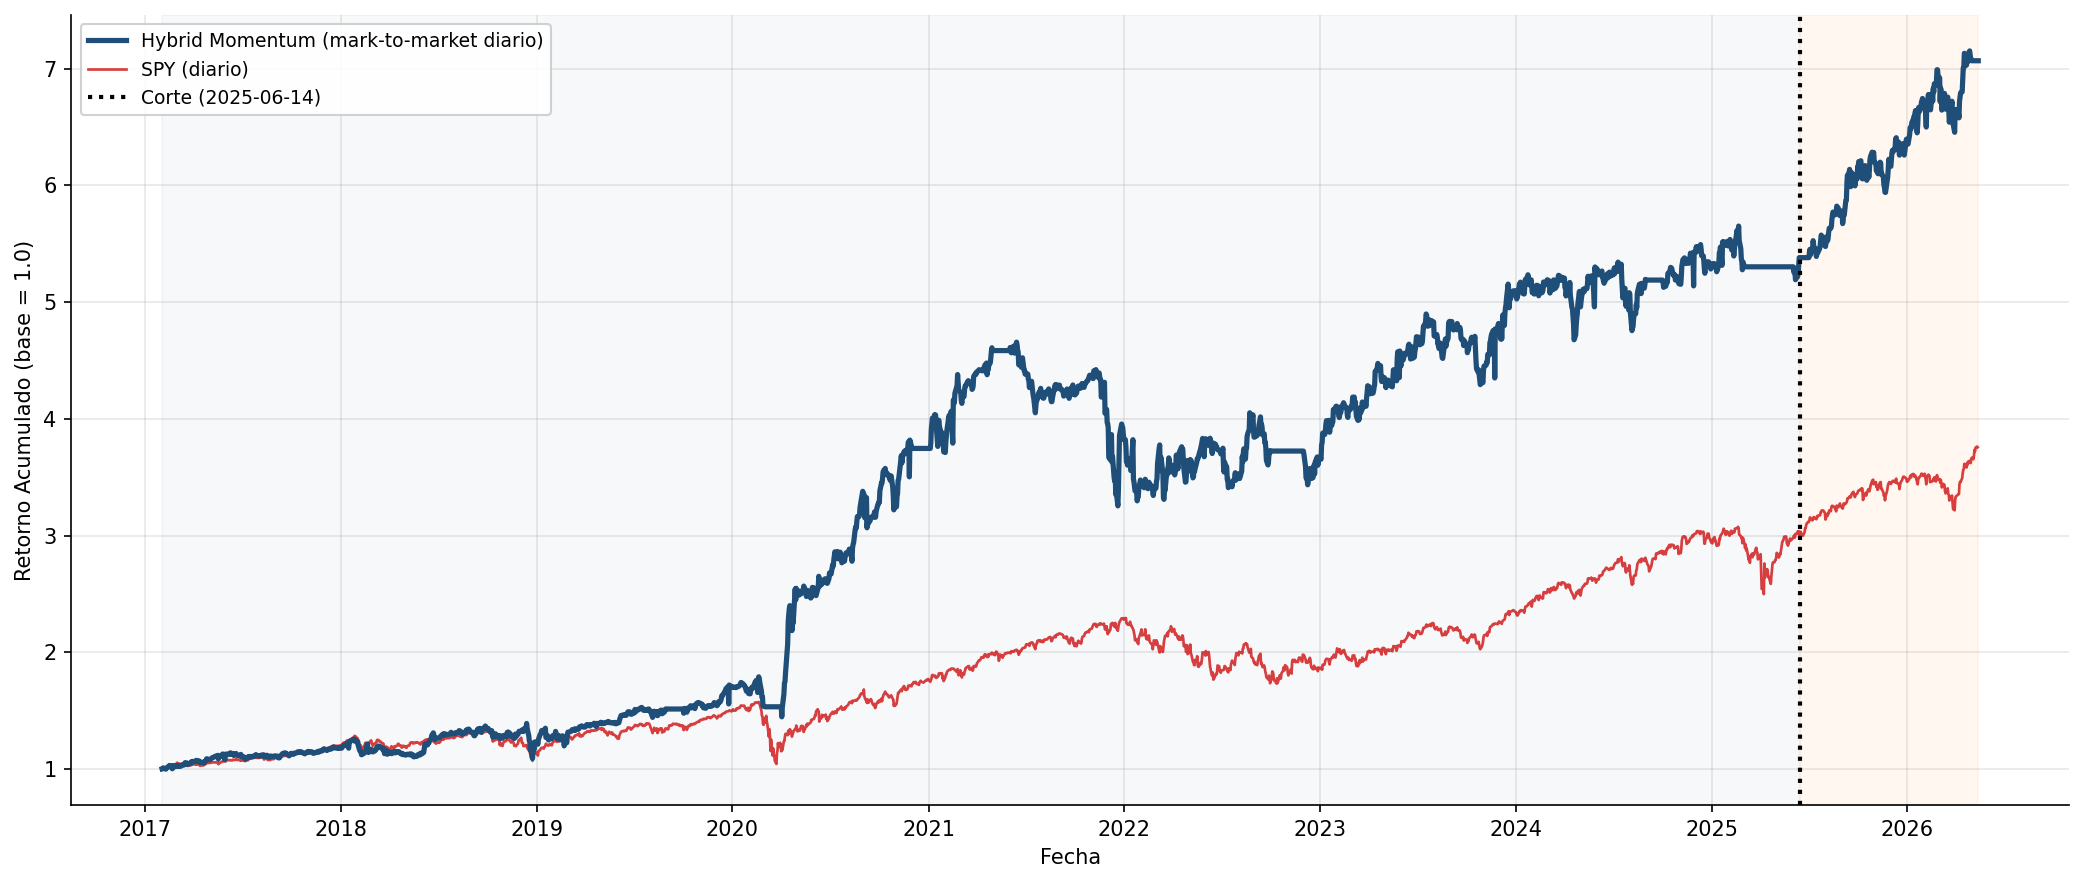
\includegraphics[width=\textwidth]{media/wf_01_equity_curve_winner_daily.png}
    \caption{Curva de capital de la mejor configuración
    en Test con resolución diaria frente al benchmark SPY.
    La línea vertical indica el inicio de la ventana de prueba.
    Fuente: Elaboración propia.}
    \label{fig:equity_winner}
\end{figure}

Se aprecia que la estrategia mantiene una trayectoria
ascendente consistente durante todo el periodo analizado,
acumulando una rentabilidad superior a la del
índice de referencia. La pendiente sostenida de la curva,
especialmente durante la ventana de prueba, sugiere que el
sistema es capaz de extraer señales de valor añadido de forma
consistente.

\paragraph{Comparativa con el índice de referencia SPY}

La Tabla~\ref{tab:comparativa_spy} presenta una comparación
entre las métricas de la mejor configuración
en Test y las del índice de referencia SPY.

\begin{table}[H]
\centering
\begin{tabular}{lrrr}
\toprule
\textbf{Métrica} & \textbf{Estrategia} & \textbf{SPY} \\
\midrule
Sharpe                & 2,113 & 0,585 \\
CAGR (\%)             & 28,47 & 12,10 \\
Caída máxima (\%)     & -4,05 & -12,10 \\
\bottomrule
\end{tabular}
\caption{Comparativa de la mejor configuración en Test frente al
benchmark SPY. Fuente: Elaboración propia.}
\label{tab:comparativa_spy}
\end{table}

La estrategia triplica prácticamente el ratio de Sharpe
del índice de referencia (2,113 frente a 0,585) y más que duplica
la rentabilidad anualizada (28,47\,\% frente a 12,10\,\%),
con una caída máxima notablemente inferior (-4,05\,\% frente a
-12,10\,\%). El sistema propuesto es capaz de generar
\textit{alpha} sobre el mercado de referencia.


\paragraph{Selección del modelo final}

Del análisis anterior se identifica como configuración de
referencia la estrategia \textbf{ALR1M\_Z} sobre el clúster 1
(Bear market rally), con rebalanceo mensual,
\texttt{top\_n=8} y ponderación equiponderada.

El criterio que justifica esta selección es:

\begin{itemize}
    \item \textbf{Rendimiento superior.} La estrategia triplica el
    Sharpe del índice de referencia (2,113 frente a 0,585) y más
    que duplica la rentabilidad anualizada (28,47\,\% frente a
    12,10\,\%), con una caída máxima de solo -4,05\,\% frente al
    -12,10\,\% del SPY.

    
\end{itemize}

No obstante, debe señalarse que este resultado excepcional
podría estar influido por las condiciones específicas del
periodo de prueba. Como alternativa más conservadora, las
configuraciones basadas en \texttt{ALR1W\_Z} ofrecen un
respaldo estadístico más amplio al concentrar nueve de las
diez posiciones del Top 10.

Los parámetros completos se resumen en la
Tabla~\ref{tab:modelo_final}.

\begin{table}[H]
\centering
\small
\begin{tabular}{ll}
\toprule
\textbf{Parámetro} & \textbf{Valor} \\
\midrule
Señal de momentum    & ALR1M\_Z (1 mes) \\
Clúster              & 1 (Bear market rally) \\
Rebalanceo           & Mensual (M) \\
Tamaño de cartera    & \texttt{top\_n=8} (8 activos) \\
Ponderación          & Equiponderada \\
Ventana anomalías    & 1 día \\
Tamaño mínimo cartera& 1 (sin mínimo exigido) \\
\bottomrule
\end{tabular}
\caption{Parámetros del modelo final seleccionado.
Fuente: Elaboración propia.}
\label{tab:modelo_final}
\end{table}


\subsubsection{Análisis de Robustez}

Esta sección aborda la cuestión de si los resultados obtenidos
pueden considerarse estadísticamente fiables o si, por el
contrario, responden a patrones 'falsos' propios del periodo de
evaluación.

\paragraph{Importancia de los hiperparámetros}

Para determinar qué parámetros del sistema ejercen una influencia
determinante sobre el rendimiento fuera de muestra, se ha
entrenado un modelo de bosque aleatorio (\textit{Random Forest})
con 300 árboles para predecir el Sharpe en prueba a partir de los
hiperparámetros de cada configuración. La
Tabla~\ref{tab:feature_importance} presenta la importancia
relativa de cada variable en la predicción.

\begin{table}[H]
\centering
\begin{tabular}{lr}
\toprule
\textbf{Variable} & \textbf{Importancia (\%)} \\
\midrule
top\_n                   & 25,99 \\
min\_portfolio\_size     & 23,64 \\
active\_cluster          & 21,01 \\
momentum\_signal         & 20,12 \\
rebalance\_freq          & 6,02  \\
rank\_weighted           & 3,22  \\
anomaly\_lookback\_days  & 0,01  \\
\bottomrule
\end{tabular}
\caption{Importancia de los hiperparámetros en la predicción del
Sharpe en Test mediante Random Forest. Fuente: Elaboración propia.}
\label{tab:feature_importance}
\end{table}

Los resultados revelan que los tres parámetros con mayor impacto
son \texttt{top\_n} (tamaño de la cartera), \texttt{min\_portfolio\_size}
(tamaño mínimo para evitar periodos en efectivo) y
\texttt{active\_cluster} (régimen de mercado seleccionado), que
conjuntamente explican más del 70\,\% de la varianza del
rendimiento fuera de muestra. La señal de momentum contribuye
con un 20\,\% adicional.

Resulta especialmente relevante la contribución prácticamente
nula del parámetro \texttt{anomaly\_lookback\_days} (ventana de
retrospectiva para el filtro DBSCAN). Este hallazgo sugiere que
la presencia del filtro topológico es importante para la
integridad del sistema, pero la longitud de la ventana de
observación de anomalías no es un factor determinante del
rendimiento, probablemente porque el filtro diario \textit{cross-
sectional} de DBSCAN proporciona una protección suficientemente
robusta con independencia del horizonte retrospectivo concreto
utilizado.

\paragraph{Sensibilidad de parámetros en ventana de prueba}

La Figura~\ref{fig:oos_sensitivity} descompone el rendimiento en Test agregado de las 1.064 configuraciones con Sharpe
de prueba válido, agrupándolas por el valor de cada
hiperparámetro. Para cada parámetro, se reconstruye la curva de
capital diaria de todas las configuraciones que comparten ese
valor y se promedia, permitiendo aislar visualmente el efecto
marginal de cada variable sobre el rendimiento conjunto.

\begin{figure}[H]
    \centering
    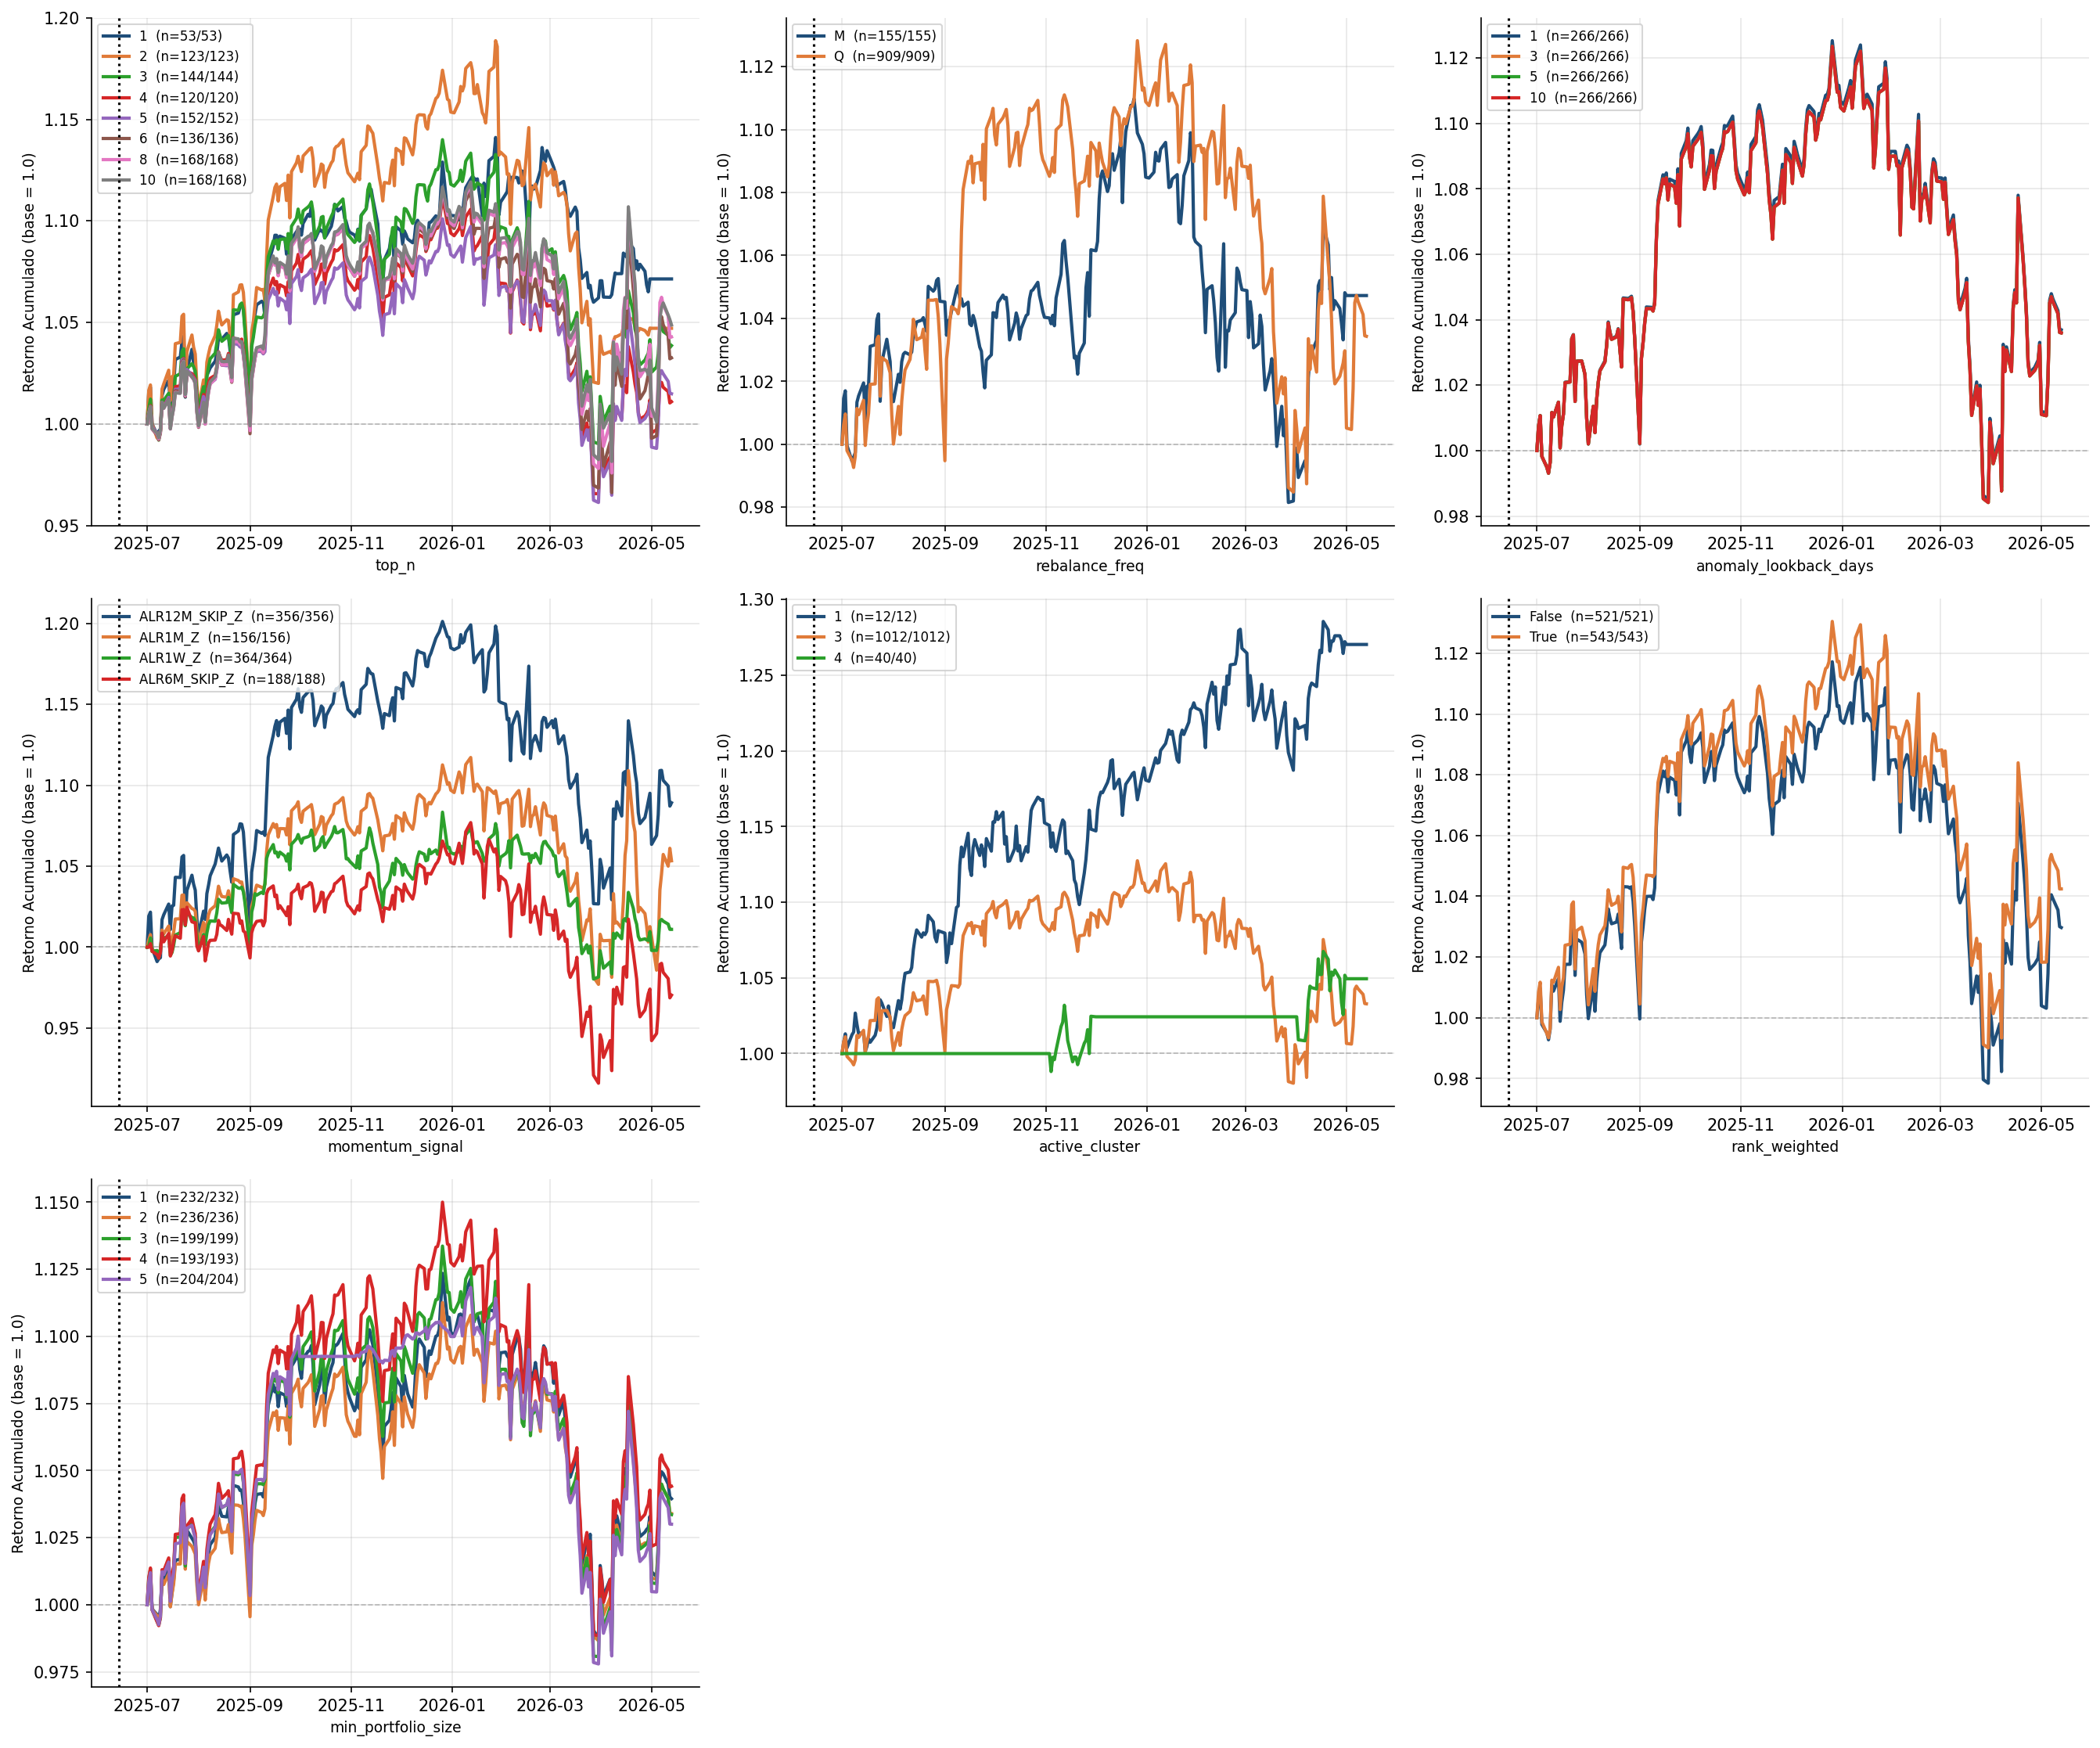
\includegraphics[width=1.05\textwidth]{media/wf_07_oos_parameter_sensitivity.png}
    \caption{Curvas de capital medias Out-of-Sample agrupadas por
    valor de hiperparámetro. Cada panel desagrega el efecto de
    una variable sobre el rendimiento agregado del conjunto de
    configuraciones (\textit{N}=1.064). Fuente: Elaboración propia.}
    \label{fig:oos_sensitivity}
\end{figure}

Se observa que:
\begin{itemize}
    
    \item \textbf{active\_cluster}: el clúster 1 es el que
    presenta el rendimiento acumulado medio más elevado (final
    de 1,270), seguido del clúster 4 (1,050). El clúster 3,
    pese a concentrar el 95\,\% de las configuraciones,
    muestra la curva media más baja (1,033).
    
    \item \textbf{rebalance\_freq}: la frecuencia mensual
    (\texttt{M}) supera a la trimestral en rendimiento acumulado
    medio (1,047 frente a 1,034), pese a que esta última
    concentra el 85\,\% de las configuraciones.
    \item \textbf{rank\_weighted}: la ponderación por ranking
    ofrece un rendimiento ligeramente superior a la
    equiponderada (1,042 frente a 1,030), aunque la diferencia
    es muy leve y ambas opciones generan rentabilidad positiva
    en promedio.
\end{itemize}

\paragraph{Conclusiones del capítulo}

Los resultados presentados a lo largo de este capítulo permiten
extraer las siguientes conclusiones consolidadas:

\begin{enumerate}
    \item \textbf{El sobreajuste existe y es significativo.} La
    mejor configuración en entrenamiento (Sharpe 1,366) presenta
    un rendimiento negativo en la ventana de prueba (\(-0,259\)).
    Este fenómeno es común a cualquier proceso de optimización
    sobre datos históricos y debe ser gestionado mediante
    validación con datos no vistos.

    \item \textbf{La robustez existe y es identificable.} El
    55,9\,\% de las configuraciones mantienen un Sharpe positivo
    en prueba, y la mejor de ellas alcanza un valor de 2,113
    (señal \texttt{ALR1M\_Z} sobre clúster 1, rebalanceo mensual,
    \texttt{top\_n=8}). Esta configuración se consolida como el
    modelo de referencia del sistema.

    \item \textbf{El sistema supera al benchmark de referencia.}
    Tanto en términos de Sharpe (2,113 frente a 0,585) como de
    CAGR (28,47\,\% frente a 12,10\,\%), la mejor configuración
    en Test triplica el rendimiento ajustado al riesgo del
    índice SPY, con una caída máxima notablemente inferior.

    \item \textbf{La selección del régimen de mercado es
    crítica.} El parámetro \texttt{active\_cluster} explica el
    21\,\% de la varianza del rendimiento fuera de muestra. El
    clúster 3 (Pullback alcista) se consolida como el régimen
    más favorable para estrategias basadas en momentum.

    \item \textbf{El filtro topológico DBSCAN es un componente
    estructural, no una variable de ajuste.} La ventana de
    retrospectiva para la detección de anomalías (\texttt{anomaly\_lookback\_days})
    presenta una importancia prácticamente nula en el modelo de
    predicción, lo que sugiere que la presencia del filtro DBSCAN proporciona una protección
    suficiente contra el ruido.
\end{enumerate}

A la vista de estos resultados, el modelo seleccionado como
configuración de referencia es la estrategia
\texttt{ALR1M\_Z} sobre el clúster 1, con rebalanceo
mensual, \texttt{top\_n=8} y ponderación equiponderada.
Esta configuración ofrece la mayor rentabilidad, superando
al índice de referencia SPY tanto en términos
de Sharpe como de rentabilidad anualizada.


\endinput
